%TODO tabellen met cijfers links uitlijnen
\documentclass[master=cws,dutch,masteroption={vs,gs},inputenc=utf8]{kulemt}
\setup{title={Vergelijkende studie van raamwerken voor de ontwikkeling van mobiele HTML5-applicaties},
  author={Tim Ameye\and Sander Van Loock},
  promotor={Prof.\,dr.\,ir.\ E. Duval},
  assessor={Prof.\,dr.\,M.\ Denecker\and F. Van Assche},
  assistant={Ir.\ G.~Parra}} 
% De volgende \setup mag verwijderd worden als geen fiche gewenst is.
\setup{filingcard,
  translatedtitle={Comparative study of frameworks for the development of mobile HTML5 applications},
  udc=681.3,
  shortabstract={Ontwikkelaars van mobiele applicaties worden geconfronteerd met een variëteit aan mobiele besturingssystemen die op smartphones en tablets aanwezig zijn.
Dit komt doordat een applicatie dient te worden geprogrammeerd aan de hand van een Software Development Kit~(SDK) die specifiek is voor het besturingssysteem.
De ontwikkeling van mobiele webapplicaties, gebruikmakend van HTML5, is een mogelijke oplossing hiervoor.
Om het ontwikkelingsproces van deze mobiele HTML5-applicaties te versnellen worden raamwerken aangeboden.
Deze helpen zowel bij het toevoegen van functionaliteit als de elementen voor de gebruikersinterface. 
Door de variëteit aan mobiele HTML5-raamwerken dringt een grondige vergelijking zich op.
Dit werk vergelijkt \st{}, \kendo{}, \jqm{} en \lungo{} op basis van vijf vergelijkingscriteria:  populariteit,  productiviteit,  gebruik,  ondersteuning en performantie.
Populariteit kijkt naar de activiteit van de raamwerken op sociale netwerken.
Productiviteit wordt opgemeten om aan te tonen hoe lang het duurt om met een raamwerk vertrouwd te raken en er daadwerkelijk iets mee te maken.
Het gebruik van de raamwerken bekijkt de elementen die het raamwerk aanbiedt.
Ondersteuning test de elementen van het raamwerk op acht verschillende mobiele apparaten.
Er wordt een evenwichtige keuze gemaakt tussen Android, iOS, smartphone en tablet.
Performantie meet enerzijds de downloadtijd en anderzijds de gebruikerservaring.
De laatstgenoemde bepaalt hoe vlot het gaat om door een lange lijst te scrollen.
De vergelijking toont aan dat \jqm{} het beste raamwerk is.
Daarna volgen \kendo{}, \lungo{} en \st{}.
\jqm{} heeft als belangrijkste troef de hoge productiviteit doordat het enerzijds zeer goed gedocumenteerd is en anderzijds geen ontwerppatroon afdwingt.
Dit laatste is echter ook een nadeel omdat het hierdoor minder scoort op gebruik.
\kendo{} heeft als troef het gebruik doordat het een ontwerppatroon afdwingt.
Het scoort echter ondermaats op performantie.
\lungo{} behaalde enkel de maximumscore voor performantie doordat \quo{}, de \js{}-bibliotheek van \lungo{},  geoptimaliseerd is voor mobiele apparaten.
\st{} is het minst productief en performant.
Daarentegen scoort \st{} het best op het vlak van gebruikerservaring.
Door het afdwingen van een ontwerppatroon scoort het quasi evengoed als \kendo{} op vlak van gebruik.
Alle onderzochte raamwerken scoren zeer goed op ondersteuning op de onderzochte mobiele apparaten.
}
}
% Verwijder de "%" op de volgende lijn als je de kaft wil afdrukken
%\setup{coverpageonly}
% Verwijder de "%" op de volgende lijn als je enkel de eerste pagina's wil
% afdrukken en de rest bv. via Word aanmaken.
%\setup{frontpagesonly}

% Kies de fonts voor de gewone tekst, bv. Latin Modern
\setup{font=lm}

% Tenslotte wordt hyperref gebruikt voor pdf bestanden.
% Dit mag verwijderd worden voor de af te drukken versie.
%\usepackage[pdfusetitle,colorlinks,plainpages=false]{hyperref}
\usepackage[pdfusetitle,plainpages=false]{hyperref}
\usepackage{kulemtx}
\headstyles{kulemtman}
\usepackage{url}

\renewcommand*\kulemtmanToC{%
\let\cftchapterfont\sffamily
\let\cftchapterdotsep\cftdotsep
\def\cftchapterleader{\normalfont\cftdotfill{\cftchapterdotsep}}%
\def\cftchapterpagefont{}%
\setlength\cftbeforechapterskip{\medskipamount}%
\setlength\cftbeforesectionskip{\smallskipamount}%
\settocdepth{section}%
\addtodef\cftchapterbreak{\par}{}%
\let\cftsubsectionfont\itshape
\def\l@subsection##1##2{%
\leftskip\cftsubsectionindent \rightskip\@tocrmarg \parfillskip\fill
\ifhmode ,\quad \else\noindent\fi \ignorespaces
{\let\numberline\@gobble \cftsubsectionfont ##1}%
~~{\cftsubsectionpagefont ##2}\ignorespaces}}
\kulemtmanToC


\usepackage{pgfplotstable} %nodig voor CSV to Latex
\usepackage{booktabs} % voor lay-out comparisontable
\usepackage{float} %floating tabellen onderdrukken
\usepackage{lscape} %tabel in landscape zetten
\usepackage{enumitem}
\usepackage{longtable} %tabel over meerdere pagina's
\usepackage{graphicx} %breedte tabel
\usepackage{subfig}
\usepackage{tocvsec2}
\usepackage{amsmath} % voor tekst in math
\newcommand{\unit}[1]{\ensuremath{\, \mathrm{#1}}} % units in math mode
\usepackage{wasysym}
\usepackage{pdfpages}

\newcommand{\term}[1]{\emph{#1}} % engelse term die niet worden vertaald naar het nederlands
\newcommand{\code}[1]{\texttt{#1}} % code command

\hyphenation{platform-onafhankelijke ontwerp-patroon}

% veelgebruikte woorden, apparaten, uitdagingen
\newcommand{\jqm}[0]{jQuery Mobile}
\newcommand{\jqma}[0]{jQM}
\newcommand{\st}[0]{Sencha Touch}
\newcommand{\sta}[0]{ST}
\newcommand{\kendo}[0]{Kendo UI}
\newcommand{\kendoa}[0]{Kendo}
\newcommand{\lungo}[0]{Lungo}
\newcommand{\lungoa}[0]{Lungo}
\newcommand{\tmp}[0]{The-M-Project}
\newcommand{\quo}[0]{QuoJS}
\newcommand{\moobile}[0]{Moobile}
\newcommand{\davinci}[0]{DaVinci}
\newcommand{\jqt}[0]{jQT}
\newcommand{\js}[0]{JavaScript}
\newcommand{\htc}[0]{HTCDesireZ}
\newcommand{\gtab}[0]{GalaxyTab}
\newcommand{\gs}[0]{GalaxyS}
\newcommand{\nexus}[0]{Nexus 7}
\newcommand{\ipadi}[0]{iPad1 WiFi}
\newcommand{\ipadiii}[0]{iPad3 4G WiFi}
\newcommand{\iphoneiii}[0]{iPhone 3GS}
\newcommand{\iphoneiv}[0]{iPhone 4S}
\usepackage{pdftexcmds}
\makeatletter
\newcommand{\uit}[1]{
	\ifnum\pdf@strcmp{#1}{anatomie}=0
  		U1:~Anatomie van pagina%
	\else\ifnum\pdf@strcmp{#1}{toestel}=0
    	U2:~Toestelspecifieke lay-out%
	\else\ifnum\pdf@strcmp{#1}{laadscherm}=0
    	U3:~Laadscherm en dialoogvenster%
	\else\ifnum\pdf@strcmp{#1}{formulieren}=0
    	U4:~Formulieren%
	\else\ifnum\pdf@strcmp{#1}{formulieren-placeholders}=0
    	U4.1:~Maak formulieren met placeholders zonder labels%
	\else\ifnum\pdf@strcmp{#1}{formulieren-types}=0
    	U4.2:~Gebruik tekst/nummer/e-mail als formuliertypes%
  	\else\ifnum\pdf@strcmp{#1}{formulieren-optieveld}=0
    	U4.3:~Optieveld%
  	\else\ifnum\pdf@strcmp{#1}{formulieren-datepicker}=0
    	U4.4:~Aangepaste datepicker met bereik van data%
  	\else\ifnum\pdf@strcmp{#1}{formulieren-monthpicker}=0
		U4.5:~Aangepaste datepicker met enkel maand- en jaarveld%
  	\else\ifnum\pdf@strcmp{#1}{formulieren-schakelaar}=0
		U4.6:~Schakelaar%
  	\else\ifnum\pdf@strcmp{#1}{formulieren-wissen}=0
		U4.7:~Wissen van een formulier%
	\else\ifnum\pdf@strcmp{#1}{vullen}=0
    	U5:~Automatisch invullen van formulier%
	\else\ifnum\pdf@strcmp{#1}{autoaanvullen}=0
    	U6:~Auto-aanvullen%
	\else\ifnum\pdf@strcmp{#1}{afbeelding}=0
    	U7:~Toevoegen van afbeelding%
	\else\ifnum\pdf@strcmp{#1}{validatie}=0
    	U8:~Formuliervalidatie%
	\else\ifnum\pdf@strcmp{#1}{handtekening}=0
    	U9:~Handtekening%
	\else\ifnum\pdf@strcmp{#1}{ajax}=0
    	U10:~AJAX%
	\else\ifnum\pdf@strcmp{#1}{lijsten}=0
    	U11:~Lijsten%
	\else\ifnum\pdf@strcmp{#1}{pdf}=0
    	U12:~Toon PDF%
	\else\ifnum\pdf@strcmp{#1}{offline}=0
  		U13:~Offline%
	\else\ifnum\pdf@strcmp{#1}{offline-data}=0
  		U13.1:~Bewaar data%
	\else\ifnum\pdf@strcmp{#1}{offline-app}=0
		U10.3:~Maak de applicatie offline beschikbaar%
  	\else
		[?]%
		
  	\fi\fi\fi\fi\fi
  	\fi\fi\fi\fi\fi
  	\fi\fi\fi\fi\fi
  	\fi\fi\fi\fi\fi
  	\fi\fi
}

\newcommand{\chal}[2]{
	\ifnum\pdf@strcmp{#1}{anatomie}=0
		C1:~Anatomy of page%
	\else\ifnum\pdf@strcmp{#1}{toestel}=0
		C2:~Device-specific layout%
  	\else\ifnum\pdf@strcmp{#1}{laadscherm}=0
		C3:~Load screen and dialog%
	\else\ifnum\pdf@strcmp{#1}{formulieren}=0
		C4:~Forms%
  	\else\ifnum\pdf@strcmp{#1}{formulieren-placeholders}=0
    	C4.1:~Create forms with placeholders without labels%
  	\else\ifnum\pdf@strcmp{#1}{formulieren-types}=0
    	C4.2:~Use the text/number/email as form types%
  	\else\ifnum\pdf@strcmp{#1}{formulieren-optieveld}=0
   	 	C4.3:~Option field%
  	\else\ifnum\pdf@strcmp{#1}{formulieren-datepicker}=0
    	C4.4:~Custom datepicker with data range%
  	\else\ifnum\pdf@strcmp{#1}{formulieren-monthpicker}=0
		C4.5:~Custom datepicker only with month and year%
  	\else\ifnum\pdf@strcmp{#1}{formulieren-schakelaar}=0
		C4.6:~Flip switch%
  	\else\ifnum\pdf@strcmp{#1}{formulieren-wissen}=0
		C4.7:~Clearing the form%
  	\else\ifnum\pdf@strcmp{#1}{vullen}=0
		C5:~Automatic form filling%
	\else\ifnum\pdf@strcmp{#1}{autoaanvullen}=0
		C6:~Autocomplete%
	\else\ifnum\pdf@strcmp{#1}{afbeelding}=0
		C7:~Attach image%
	\else\ifnum\pdf@strcmp{#1}{validatie}=0
		C8:~From validation%
	\else\ifnum\pdf@strcmp{#1}{handtekening}=0
		C9:~Signature%
	\else\ifnum\pdf@strcmp{#1}{ajax}=0
		C10:~AJAX%
  	\else\ifnum\pdf@strcmp{#1}{lijsten}=0
		C11:~Lists%
  	\else\ifnum\pdf@strcmp{#1}{pdf}=0
		C12:~Show PDF%
  	\else\ifnum\pdf@strcmp{#1}{offline}=0
		C13:~Offline%
  	\else\ifnum\pdf@strcmp{#1}{offline-data}=0
  		C13.1:~Saving data%
  	\else\ifnum\pdf@strcmp{#1}{offline-app}=0
  		C13.2:~Making app offline%
	\else
    	[?]%
	
  	\fi\fi\fi\fi\fi
  	\fi\fi\fi\fi\fi
  	\fi\fi\fi\fi\fi
  	\fi\fi\fi\fi\fi
  	\fi\fi
}
\makeatother

\begin{document}

% \begin{preface}
%   Dit is mijn dankwoord om iedereen te danken die mij bezig gehouden heeft.
%   Hierbij dank ik mijn promotor, mijn begeleider en de voltallige jury.
%   Ook mijn familie heeft mij erg gesteund natuurlijk.
% \end{preface}

\chapter*{Dankwoord Tim}
Ik wil in eerste plaats mijn promotor prof. E.~Duval en het bedrijf Capgemini bedanken voor het interessante onderwerp.
Daarnaast wil ik G.~Parra bedanken voor de wekelijkse meetings en de vele inzichten die hij verschafte doorheen het academiejaar.
Ook het nalezen van de gehele thesis tezamen met S.~Charleer verdient een woordje van dank.
Vervolgens was er ook begeleiding vanuit Capgemini door J.~Verhulst en J.~Persoons die naast hun job tijd maakten voor het ondersteunen van deze thesis.
Ook wil ik de lezers van onze thesisblog bedanken voor de inspirerende commentaren die ze verschaften.

In het bijzonder dank ik mijn thesispartner Sander die samen met mij deze thesis tot een goed einde heeft gebracht.
Ik bedank ook Koen voor de vele diepe gesprekken en verlichtende momenten. 
Niet enkel hen, maar ook vele andere goede vrienden zowel binnen als buiten de richting Computerwetenschappen dienen te worden beloond met een welgemeende dankjewel.
Daarnaast wil ik mijn vriendin Marjan bedanken omdat ze er steeds was voor mij.
Als laatste maar daarom niet minder belangrijk dank ik mijn ouders, want zonder hen was dit nooit mogelijk geweest.

\chapter*{Dankwoord Sander}
Bij het maken van deze thesistekst hebben letterlijk en figuurlijk bloed, zweet en tranen gevloeid.
Het resultaat na één jaar hard werken mag dan ook gezien worden.
Meerdere mensen hebben hier natuurlijk toe bijgedragen.
Eerst zou ik prof. E.~Duval willen bedanken voor het interessante onderwerp dat hij in samenwerking met Capgemini beschikbaar stelde.
Hierbij wil ik ook Jan en Jannik van Capgemini bedanken om deze thesis mee te ondersteunen.
Verder was de hulp van onze begeleider,  Gonzalo,  onmisbaar.
Dear Gonzalo,  thanks for all the comments,  remarks and opinions that you gave us every week.
These definitely brought the quality of this text to a higher level.

De steun van mijn ouders zorgde ervoor dat ik een heel jaar ongestoord kon werken.
Ook bedankt voor de steun die jullie mij gaven om mijn diploma te halen.
Maaike,  ik weet dat je me moest missen als ik tijdens het weekend aan mijn thesis moest werken.
Ik vind het super dat je zo geduldig was en hoop alle verloren tijd snel in te halen!
Ook is een eervolle vermelding van Gunther Desamblanx op zijn plaats.
Samen met Simon de producer zorgde je elke weekdag tussen 22u en 24u voor de meest productieve uren.

Tot slot wil ik mijn thesispartner, Tim,  bedanken voor het geweldige jaar dat we samen hebben meegemaakt.
Jouw stipheid, nauwkeurigheid en gedrevenheid zijn niet te onderschatten!
Ik zal onze nachtelijke discussies nooit vergeten.
Je was een fijne collega,  ik wens je het allerbeste voor je doctoraat!

\tableofcontents*

\begin{abstract}
Ontwikkelaars van mobiele applicaties worden geconfronteerd met een variëteit aan mobiele besturingssystemen die op smartphones en tablets aanwezig zijn.
Dit komt doordat een applicatie dient te worden geprogrammeerd aan de hand van een Software Development Kit~(SDK) die specifiek is voor het besturingssysteem.
De ontwikkeling van mobiele webapplicaties, gebruikmakend van HTML5, is een mogelijke oplossing hiervoor.
Om het ontwikkelingsproces van deze mobiele HTML5-applicaties te versnellen worden raamwerken aangeboden.
Deze helpen zowel bij het toevoegen van functionaliteit als de elementen voor de gebruikersinterface. 

Door de variëteit aan mobiele HTML5-raamwerken dringt een grondige vergelijking zich op.
Dit werk vergelijkt \st{}, \kendo{}, \jqm{} en \lungo{} op basis van vijf vergelijkingscriteria:  populariteit,  productiviteit,  gebruik,  ondersteuning en performantie.
Populariteit kijkt naar de activiteit van de raamwerken op sociale netwerken.
Productiviteit wordt opgemeten om aan te tonen hoe lang het duurt om met een raamwerk vertrouwd te raken en er daadwerkelijk iets mee te maken.
Het gebruik van de raamwerken bekijkt de elementen die het raamwerk aanbiedt.
Ondersteuning test de elementen van het raamwerk op acht verschillende mobiele apparaten.
Er wordt een evenwichtige keuze gemaakt tussen Android, iOS, smartphone en tablet.
Performantie meet enerzijds de downloadtijd en anderzijds de gebruikerservaring.
De laatstgenoemde bepaalt hoe vlot het gaat om door een lange lijst te scrollen.

De vergelijking toont aan dat \jqm{} het beste raamwerk is.
Daarna volgen \kendo{}, \lungo{} en \st{}.
\jqm{} heeft als belangrijkste troef de hoge productiviteit doordat het enerzijds zeer goed gedocumenteerd is en anderzijds geen ontwerppatroon afdwingt.
Dit laatste is echter ook een nadeel omdat het hierdoor minder scoort op gebruik.
\kendo{} heeft als troef het gebruik doordat het een ontwerppatroon afdwingt.
Het scoort echter ondermaats op performantie.
\lungo{} behaalde enkel de maximumscore voor performantie doordat \quo{}, de \js{}-bibliotheek van \lungo{},  geoptimaliseerd is voor mobiele apparaten.
\st{} is het minst productief en performant.
Daarentegen scoort \st{} het best op het vlak van gebruikerservaring.
Door het afdwingen van een ontwerppatroon scoort het quasi evengoed als \kendo{} op vlak van gebruik.
Alle onderzochte raamwerken scoren zeer goed op ondersteuning op de onderzochte mobiele apparaten.
\end{abstract}


\selectlanguage{english}
\begin{abstract}
Developers of mobile applications are confronted with a variety of mobile operating systems that are present on smartphones and tablets.
This is because an application has to be programmed with a Software Development Kit~(SDK) specific for the operating system.
Developing mobile web applications using HTML5 can be a solution for this problem.
To speed up development,  frameworks are presented.
These help to add functionality and elements for the user interface.

Because of the variety of mobile HTML5 frameworks,  a thorough comparative study is necessary.
This thesis compares \st{}, \kendo{}, \jqm{} and \lungo{} based on five comparison criteria:  popularity,  productivity,  usage,  support and performance.
Popularity looks at the activity of frameworks on social networks.
Productivity is determined by measuring how long it takes to get acquainted with the framework and build something useful. 
Next, usage of the framework is studied by looking which elements are offered by the framework.
Support tests the elements of the framework on eight different devices.
A good balance is made between Android, iOS, smartphone and tablet.
Performance measures the download time and user experience.
The latter is determined by the smoothness of scrolling through a long list.

The comparison shows that \jqm{} is the best framework followed by \kendo{},  \lungo{} and \st{}.
\jqm{} is highly productive,  a major advantage because on the one hand it is well-documented and on the other hand it does not impose an architecture.
The latter,  however,  becomes a disadvantage when looking at the usage.
\kendo{} has usage as most important advantage because it imposes an architecture.
However,  it scores inferior on performance.   
\lungo{} only achieves a maximum score for performance because \quo{},  the underlying \js{} library,  is optimized for mobile devices.
\st{} is the least productive and performant.
By contrast,  \st{} scores the best in user experience.
By enforcing an architecture,  it scores almost as good as \kendo{} regarding usage.
All frameworks score good for support on the evaluated mobile devices.

\end{abstract}
\selectlanguage{dutch}

% Een lijst van figuren en tabellen is optioneel
\listoffigures
\listoftables
% Bij een beperkt aantal figuren en tabellen gebruik je liever het volgende:
%\listoffiguresandtables

\chapter{Lijst van afkortingen}
\begin{flushleft}
  \renewcommand{\arraystretch}{1.1}
  \begin{longtable}{p{2cm} l}
     AHP & Analytic Hierarchy Process \\
     AJAX & Asynchronous JavaScript And XML \\
     API & Application Programming Interface \\
     ASP & Active Server Pages \\
     BS & BesturingsSysteem \\
     CORS & Cross-Origin Resource Sharing \\
     CPU & Central Processing Unit \\
     CRUD & Create Read Update Destroy \\
     CSS(3) & Cascading Style Sheets (3) \\
     DOM & Document Object Model \\
     EDGE & Enhanced Data Rates for GSM Evolution \\
     (G)GI & (Grafische) GebruikersInterface \\
     GNU GPL & GNU's Not Unix General Public License \\
     GPRS & General Packet Radio Service \\
     GPS & Global Positioning System \\
     GPU & Graphics Processing Unit \\
     HSDPA & High-Speed Downlink Packet Access \\
     HTML(5) & HyperText Markup Language (5) \\
     IDE & Integrated Development Environment \\
     ISO & International Organization for Standardization \\
     \jqma{} & \jqm{} \\
     JSON(P)  & JavaScript Object Notation (with Padding) \\
     JSP & JavaServer Pages \\
     \kendoa{} & \kendo{} \\
     LTE & Long Term Evolution \\
     \lungoa{} & \lungo{} \\
     MIT & Massachusetts Institute of Technology \\
     MVC & Model-View-Controller \\
     MVVM & Model-View-View Model \\
     OEM & Original Equipment Manufacturer \\
     PCAP & Packet CAPture \\
     PDA & Personal Digital Assistant \\
     PDF & Portable Document Format \\
     PHP & PHP: Hypertext Preprocessor \\
     POC & Proof Of Concept \\
     PPI & Pixels Per Inch \\
     QR & Quick Response \\
     RAM & Random Access Memory \\
     RWD & Responsive Web Design \\
     SASS & Syntactically Awesome StyleSheets \\
     SDK & Software Development Kit \\
     SEO & Search Engine Optimization \\
     SMS & Short Message Service \\
     \sta{} & \st{} \\
     USB & Universal Serial Bus \\
     UTMS & Universal Mobile Telecommunications System \\
     W3C & World Web Consortium \\
     WHATWG & Web Hypertext Application Technology Working Group \\
     WORA & Write Once, Run Anywhere \\
     WYSIWYG & What You See Is What You Get \\
     X(HT)ML & eXtensible (HyperText) Markup Language \\ 
  \end{longtable}
\end{flushleft}

% Nu begint de eigenlijke tekst
\mainmatter

\chapter{Inleiding} %3 blz (0.75 per sectie)
\label{inleiding}
%In dit hoofdstuk wordt het werk ingeleid. Het doel wordt gedefinieerd en er wordt uitgelegd wat de te volgen weg is (beter bekend als de rode draad).

%\section{Achtergrondinformatie} %tim
% - web apps (cross platform)
% - HTML5/js/css3
% - wat doet framework?
% - om de ontwikkeling vergemakkelijk worden frameworks aangeboden... 

Het gebruik van smartphones en tablets stijgt ontzettend snel in onze samenleving.
Waar voorheen met de gsm enkel kon worden gebruik gemaakt van de voorgeïnstalleerde applicaties op het apparaat, kunnen op deze mobiele apparaten ook extra applicaties vanuit een winkel worden gedownload en geïnstalleerd.
Ontwikkelaars van deze mobiele applicaties worden geconfronteerd met de variëteit aan mobiele besturingssystemen die op deze apparaten aanwezig zijn.
% Er bestaat niet enkel verschillende besturingssystemen, maar ook verschillende versies van besturingssystemen.
Dit komt doordat een applicatie dient te worden geprogrammeerd in een programmeertaal die specifiek is tot het besturingssysteem.
Ontwikkelaars zullen dus eenzelfde applicatie in verschillende programmeertalen dienen te programmeren om een zo groot mogelijk publiek te bereiken.
Niet enkel het programmeren, maar ook het onderhoud van de applicaties in verschillende programmeertalen brengt een grote kost met zich mee.

Een oplossing hiervoor is het maken van een mobiele webapplicatie, gebruikmakend van HTML5.
Ten eerste wordt deze rechtstreeks in een webbrowser geopend en moet dus niet langer worden geïnstalleerd vanuit een winkel.
Dit betekent dus dat ieder mobiel apparaat die een webbrowser heeft, de webapplicatie kan openen ongeacht zijn mobiel besturingssysteem.
Ten tweede wordt de applicatie slechts in één programmeertaal geschreven, wat de kost omlaag brengt.
Om het ontwikkelingsproces van deze mobiele HTML5-applicaties te versnellen worden raamwerken aangeboden die helpen bij de functionaliteit van de applicatie en de elementen voor de gebruikersinterface. 

\section{Probleembeschrijving} %tim
% - heel veel frameworks, nog geen literatuur die vergelijkt (alleen blogs e.d.)
% - eerder voorstelling ipv objectieve verglijking.
% - beste framework?
% - hoe vergelijken?
Mobiele HTML5-raamwerken schieten als paddenstoelen uit de grond en ook de verschillende versies van eenzelfde raamwerk volgen elkaar in snel op.
In de huidige literatuur worden er vaak raamwerken aangehaald en besproken, maar niet vergeleken.
Indien deze toch worden vergeleken, gebeurt dit vaak subjectief of worden punten gegeven zonder een gestaafde methode te gebruiken.
Geen enkele literatuur bouwt verder op reeds bestaande literatuur van vergelijkingen voor HTML5-raamwerken of aggregeert de losstaande vergelijkingen tot één geheel.

\section{Doelstellingen} %sander
% Is er een beste framework?
% contribuite:  methodologie uitwerken om OBJECTIEF en VISUEEL raamwerken te vergelijken
Deze thesistekst bestaat uit twee grote doelstellingen die beide in de titel verborgen zitten.
Een eerste doel is het creëren van een methodologie om HTML5-raamwerken met elkaar te vergelijken.
Deze methodologie moet alle belangrijke aspecten van de raamwerken tegen het licht houden.
Ook moet er geprobeerd worden de werkwijze zo objectief mogelijk te laten verlopen en het resultaat van de studie op een eenvoudige,  visuele manier aan de lezer te presenteren.
Het tweede doel omdat de effectieve vergelijking van de raamwerken zelf.
Door de grote verscheidenheid van HTML5-raamwerken moeten de bestudeerde raamwerken zo worden gekozen dat ze zoveel mogelijk aspecten van alle raamwerken bevatten.
Hier komt ook de afweging tussen het aantal bestudeerde raamwerken en diepte van de vergelijkende studie de kop op steken.
De raamwerken die worden gekozen moeten vervolgens worden vergeleken met de vooropgestelde methodologie.
Het resultaat moet alle positieve en negatieve aspecten van de raamwerken bevatten.
Vervolgens moeten er gekeken worden of er één raamwerk het best is of er verschillende raamwerken in verschillende situaties als best kunnen worden bestempeld.

\section{Toepassingsgebied} %sander
% mobiele wereld (mobile = booming)
% web (web = booming)
% kruising tussen web en mobile = super booming!
% bedrijfswereld (capgemini) HTML5 iets nieuws,  bedrijven kunnen nu een met een gerust hart een goede keuze maken (mss beter doelstellingen)
HTML5-raamwerken vergemakkelijken de ontwikkeling van HTML5-applicaties.
Deze applicaties zijn toepasbaar op twee domeinen: web en mobiel.
Ze zijn toegankelijk via het web en geoptimaliseerd om op mobiele apparaten te kunnen werken.
Het aanspreken van mobiele applicaties via het web heeft zowel voor- als nadelen.
Zeker wanneer er wordt vergeleken met \term{native} of hybriede applicaties.
De focus van deze studie ligt echter niet bij het onderzoeken van deze voor- of nadelen!
Wel zullen de verschillende technologieën besproken worden om mobiele applicaties te maken.

Omdat Capgemini deze thesis mee ondersteunt zullen beide domeinen vanuit een bedrijfscontext worden benaderd.
Dit zal vooral naar boven komen in de keuze van vergelijkingscriteria en de methode om deze criteria te testen.


%\section{Rode draad} %tim
% - geen nadruk op passief actief
% - passieve en actieve vergelijkingscriteria al hier vermelden.
Eerst wordt in hoofdstuk~\ref{chap:literatuurstudie} de basis van dit werk uitgelegd.
Vervolgens wordt er in hoofdstuk~\ref{chap:raamwerken} een passieve vergelijking gedaan van de gekozen raamwerken.
Daarna zullen in hoofdstuk~\ref{chap:vergelijkingscriteria} de gekozen vergelijkingscriteria voor de actieve vergelijking aan bod komen en verantwoord worden.
Hieropvolgend wordt in hoofdstuk~\ref{chap:evaluatie} deze actieve vergelijking uitgevoerd op de gekozen raamwerken aan de hand van de gekozen criteria.
Als laatste wordt dit alles besloten in hoofdstuk~\ref{chap:besluit}.

%%% Local Variables: 
%%% mode: latex
%%% TeX-master: "masterproef"
%%% End: 

\chapter{Literatuurstudie}
\label{chap:literatuurstudie}
In dit hoofdstuk wordt gestart met het bekijken welke mobiele apparaten er allemaal bestaan (\ref{sec:mobiele-apparaten}). 
Vervolgens wordt er gekeken wat er onder de motorkap van deze apparaten zit, namelijk welke mobiele besturingssystemen (\ref{sec:mobiele-besturingssystemen}), welke mobiele applicaties (\ref{sec:mobiele-applicaties}) en welke mobiele webbrowsers (\ref{sec:mobiele-webbrowsers}) er bestaan. 
Daarna komen de drie bouwblokken van het web aan bod (\ref{sec:html5-css3-js}), namelijk HTML, CSS en \js{}.
Hierna wordt ingegaan op bestaande mobiele HTML5-raamwerken (\ref{sec:mobiele-html5-raamwerken}).  
Ten slotte worden verschillende, reeds bestaande manieren om raamwerken te vergelijken, bekeken (\ref{sec:vergelijken-raamwerken}).

%%%%%%%%%%%%%%%%%%%%%%%%%%%%%%%%%%%%%%%%%%%%%%%%%%%%%%%%%%%%%%%%%%
%%%%%%%%%%%%%%%%%%%%%%%%%%%%%%%%%%%%%%%%%%%%%%%%%%%%%%%%%%%%%%%%%%

\section{Mobiele apparaten}
\label{sec:mobiele-apparaten}
Mobiele apparaten bestaan in alle soorten en maten, met weinig of veel opties, voor weinig of veel geld zoals wordt geïllustreerd op figuur \ref{fig:devices}. 
Het verdient daarom de aandacht om deze diversiteit onder de loep te nemen. 
Eerst wordt ingegaan op drie soorten mobiele apparaten, namelijk de smartphone, tablet en e-reader~\cite{GCF2013}.
Daarna wordt stilgestaan bij de kenmerken van deze apparaten~\cite{PhilDutson2012}.

\begin{figure}
  \centering
  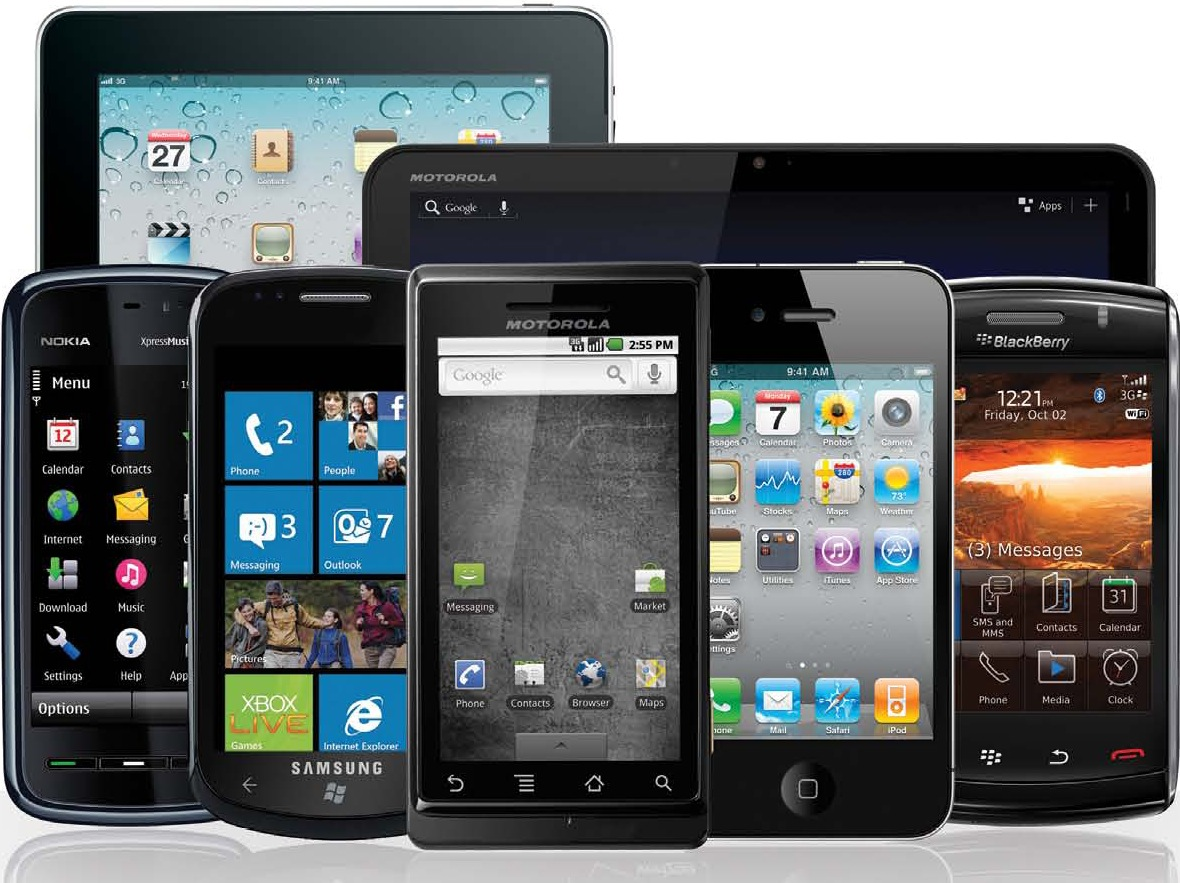
\includegraphics[height=0.6\textwidth]{figuren/mobile-devices.jpg}
  \caption{Verschillende mobiele apparaten~\cite{Grady2013}.}
  \label{fig:devices}
\end{figure}

\subsection{Soorten}
Sinds de voorstelling van de Apple iPhone in 2007~\cite{David2011}, stijgt het gebruik van de smartphone ontzettend snel in onze samenleving.  
Momenteel zijn er al meer dan 1 miljard smartphones in gebruik~\cite{Yang2012}. 
Dit zal tegen 2015 verdubbeld zijn~\cite{Gillett2012}.
Foto's of video's nemen, navigeren naar het dichtstbijzijnde restaurant of nog snel het weer voor de komende dagen opzoeken, het is allemaal mogelijk. 
Hoewel Apple de lat hoog heeft gelegd met het uitbrengen van de iPhone, zijn er ook nog andere spelers op de markt. 
Zo zijn er bijvoorbeeld de op Google's Android gebaseerde smartphones zoals de Nexus 4 en de op Windows Phone gebaseerde smartphones zoals de Nokia Lumia 800.

De tweede soort mobiele apparaten zijn tablets.
Tegen 2016 zulen er 760 miljoen tablets in gebruik zijn~\cite{Gillett2012}.
Ook hier kan terug gedacht worden aan één van Apple's succesvolle producten, namelijk de in 2010 uitgebrachte iPad~\cite{Apple2010}. 
Er dient echter wel opgemerkt te worden dat tien jaar voordien, Microsoft al eerder een tablet uitbracht met veel minder succes~\cite{Microsoft2000}.

%TODO voor sander: wat denk je er van om e-reader er uit smijten dan gewoon kort zeggen dat er nog PDA's, e-readers, enz bestaan? bij de kenmerken vertel ik toch enkel dingen over smartphone en tablet, dus die e-reader doet er niet echt toe..
De \term{e-reader} behoort tot de laatste categorie van mobiele apparaten. 
Deze wordt hoofdzakelijk gebruikt om digitale boeken te lezen, maar betere modellen laten bijvoorbeeld ook toe om te surfen op het Internet. 
Ook hier bestaat er een variëteit aan modellen zoals de Kindle van Amazon en de Reader van Sony.

\subsection{Kenmerken}
Door de vele verschillende soorten en modellen aan mobiele apparaten, is het nodig om op een hoog niveau te bekijken over welke kenmerken deze allemaal (kunnen) beschikken. 
Bij deze bespreking wordt ingegaan op de voornaamste kenmerken van smartphones en tablets. 
De kenmerken en tekst zijn gebaseerd op Phil Dutson~\cite{PhilDutson2012}.

\subsubsection{Resolutie en PPI}
Een eerste kenmerk waar vooral Apple met haar Retina graag mee uitpakt, is de resolutie. 
Dit is het aantal pixels getoond op het beeldscherm en wordt uitgedrukt in breedte $\times$ hoogte. 
Hoe kleiner, hoe minder er op het scherm kan worden getoond. 
Dit is vooral belangrijk wanneer veel informatie op het scherm wordt getoond. 
Bij een een kleine resolutie dient er gescrold te worden om te rest van de informatie te zien.
%Een overzicht van resoluties van bekende mobiele apparaten wordt getoond op de figuur \ref{fig:resoluties}.

Indien er naast de resolutie ook nog eens rekening wordt gehouden met de fysieke grootte van het scherm, wordt er gesproken over pixels per inch~(PPI). 
De eerste iPhone had een resolutie van 320$\times$480 en een 3,5” scherm, wat neerkomt op 163 PPI. 
De iPhone~4 (Retina) daarentegen heeft een resolutie van 640$\times$960 en een 3,5” scherm, wat neerkomt op 326 PPI. 
Met andere woorden zijn er meer pixels op dezelfde fysieke grootte geplaatst, wat een scherper beeld tot resultaat heeft. 

%TODO aan Sander: is deze afbeelding nuttig?  ik zou dan eerder een figuur met allemaal verschillende devices in mijn thesis steken dan een afbeelden met deze resoluties...
%\begin{figure}
%  \centering
%  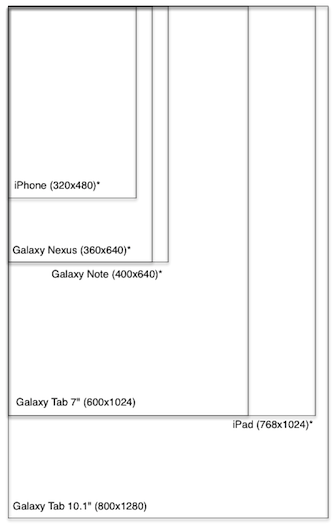
\includegraphics[height=0.8\textwidth]{figuren/mobile-devices-resolutions.png}
%  \caption{Resoluties van bekende mobiele apparaten~\cite{Wolfermann2012}.}
%  \label{fig:resoluties}
%\end{figure}

\subsubsection{Aanraakscherm}
De populaire soorten schermen zijn resistieve en capacitieve aanraakschermen. 
De eerstgenoemde soort maakt gebruik van twee lagen die gescheiden worden door een tussenruimte. 
Door druk ontstaat er contact tussen de twee lagen. 
Meestal wordt bij deze soort schermen een stylus meegeleverd. 

De laatstgenoemde soort maakt gebruik van veranderingen in frequentie. 
Door het scherm aan te raken met een vinger, dat een geleider is, ontstaat er een kleine verandering in frequentie die gedetecteerd wordt. 
Niet-geleidende materialen zullen geen frequentieverandering veroorzaken, wat verklaart dat zo'n scherm niet reageert als het wordt aangeraakt met een handschoen.

\subsubsection{Camera}
Praktisch ieder recent mobiele apparaat is uitgerust met een camera. 
Sommige bevatten zelfs twee camera's. 
De camera vooraan is veelal van mindere kwaliteit en wordt gebruikt om videogesprekken te voeren. 
Achteraan het apparaat zit dan een camera met hogere resolutie om foto's van betere kwaliteit te kunnen maken.

Twee voorbeelden van toepassingen van de camera zijn toegevoegde realiteit en het inscannen van barcodes.
Bij het eerstgenoemde wordt informatie toegevoegd aan het beeld dat door de camera wordt geregistreerd.
Het laatstgenoemde wordt gebruikt om de populaire QR-code in te scannen en te zien wat ze betekent.
Zo'n code kan tekst bevatten, een link naar een website, een telefoonnummer, enzovoort. 

\subsubsection{Verbinding}
Iedereen wil zoveel mogelijk met elkaar en het Internet verbonden zijn en dit kan ook op mobiele apparaten. 
Enerzijds kan gebruik worden gemaakt van mobiel Internet en anderzijds van draadloos Internet.
Daarnaast kan data ook uitgewisseld worden tussen apparaten, zonder hiervoor het Internet te gebruiken.
Een voorbeeld hiervan is Bluetooth dat een draadloze verbinding op korte afstand opzet.

\paragraph{Mobiel Internet}
Om dit in perspectief te plaatsen wordt eerst even teruggegaan in de tijd van mobiele communicatie.
Helemaal in het begin was er 1G, de eerste generatie mobiele telefonie, waarbij gesprekken analoog werd verzonden.
2G gebruikte daarentegen een digitaal netwerk, waarbij nieuwe diensten zoals SMS tekstberichten beschikbaar werden~\cite{Miami2008}.

Op de overgang van 2G naar 3G worden General Packet Radio Service~(GPRS) en Enhanced Data Rates for GSM Evolution~(EGDE) geplaatst.
GPRS is een uitbereiding op 2G waarbij data over het mobiele netwerk kan worden uitgewisseld.
De gebruiker moet slechts één maal inbellen op het netwerk en blijft daarna altijd verbonden.
Omdat niet alle telecomproviders hun hardware wilden aanpassen naar 3G, gebruikten ze EGDE dat een uitbreiding is op GPRS en grotere snelheden mogelijk maakt~\cite{Lauwers2007}.

3G maakt gebruikt van een volledige nieuwe technologie, namelijk Universal Mobile Telecommunications System~(UTMS).
Het is dus niet langer een uitbreiding op het bestaande netwerk zoals dat voor GPRS het geval was.
De vraag naar bandbreedte blijft, waardoor High-Speed Downlink Packet Access~(HSDPA) werd ontwikkeld. 
Het is een nieuwe implementatie van UTMS dat nog grotere snelheden toelaat~\cite{Lauwers2007}.

Op dit moment zijn telecomoperatoren volop bezig met de uitrol van 4G.
Dit moet nog grotere snelheden mogelijk maken door gebruik te maken van LTE Advanced, een verbetering van Long Term Evolution~(LTE).

\paragraph{Draadloos Internet}
Net zoals laptops draadloos verbinden met Internet via Wifi, kan dit ook op mobiele apparaten.
Vaak is de kost van mobiel Internet groter dan die van draadloos Internet, waardoor dit type van verbinding de voorkeur krijgt.

\subsubsection{GPS}
Met het \term{global positioning system} (GPS) kan de gebruiker zijn locatie opvragen en doorgeven aan een applicatie om zo bijvoorbeeld het dichtstbijzijnde restaurant te vinden. 
Doordat het wat kan duren vooraleer de locatie is vastgesteld via GPS, kan het mobiel apparaat ook gebruik maken van mobiele masten of het Internet om zo, hetzij minder nauwkeurig, sneller de locatie te bepalen.

%%%%%%%%%%%%%%%%%%%%%%%%%%%%%%%%%%%%%%%%%%%%%%%%%%%%%%%%%%%%%%%%%%
%%%%%%%%%%%%%%%%%%%%%%%%%%%%%%%%%%%%%%%%%%%%%%%%%%%%%%%%%%%%%%%%%%

\section{Mobiele besturingssystemen}
\label{sec:mobiele-besturingssystemen}
Net zoals er brede waaier bestaat aan besturingssystemen voor computers, geldt dit ook zo voor mobiele apparaten. 
In deze sectie wordt een overzicht gegeven van mobiele besturingssystemen met een significant marktaandeel~\cite{David2011, Hales2012} zoals iOS en Android, maar ook een nieuwkomer op de markt, namelijk Windows Phone.
iOS en Android haalden respectievelijk 14,9\% and 75,0\% in het derde kwartaal van 2012.
Windows Phone haalt 2\% van het marktaandeel binnen in datzelfde kwartaal~\cite{Protalinski2012}.

Bij ieder besturingssysteem zal ook over de winkel gepraat worden waar applicaties kunnen worden gevonden.
Net zoals programma's geïnstalleerd worden op een computer, kan dit ook voor mobiele apparaten.
Deze aangeboden applicaties worden verzameld in een winkel waarna de gebruiker ze, al dat niet gratis, kan downloaden en installeren.
De winkel kan de kwaliteit van deze applicaties hoog houden door regels op te leggen aan de ontwikkelaars (zie \ref{sec:mobiele-applicaties}).

\begin{table}[t]
\centering
\pgfplotstabletypeset[
  begin table=\begin{tabular}{l l},
  end table=\end{tabular},
  col sep=comma,
  header=true,
  string type,
  skip coltypes=true,
  columns={Versie,Marktaandeel},
  columns/Versie/.style={column name=\textbf{iOS}},  
  columns/Marktaandeel/.style={column name=\textbf{Marktaandeel (\%)}},
  every head row/.style={
    before row=\toprule,
    after row=\midrule},
  every last row/.style={
    after row=\bottomrule}
]{tabellen/ios.csv}
\quad
\pgfplotstabletypeset[
  begin table=\begin{tabular}{l l},
  end table=\end{tabular},
  col sep=comma,
  header=true,
  string type,
  skip coltypes=true,
  columns={Versie,Marktaandeel},
  columns/Versie/.style={column name=\textbf{Android}},  
  columns/Marktaandeel/.style={column name=\textbf{Marktaandeel (\%)}},
  every head row/.style={
    before row=\toprule,
    after row=\midrule},
  every last row/.style={
    after row=\bottomrule}
]{tabellen/android.csv}
\caption{Marktaandeel van iOS-versies op 8 mei 2013 en Android-versies op 1 mei 2013.  \protect\cite{Smith2013,Android2013}.}
\label{tabel:marktaandeel-ios-android}
\end{table}

\subsection{iOS}
Het iPhone-besturingssysteem is voor het eerst uitgekomen in juni 2007 tezamen met de iPhone. 
Later werd het hernoemd naar iPhone OS en uiteindelijk werd het iOS. 
Het is duidelijk dat iOS gebonden is aan de hardware van Apple. 
Verschillende versies volgden elkaar op: iOS 2 (juli 2008), iOS 3 (juni 2009), iOS 4 (juni 2010) en iOS 5 (oktober 2011)~\cite{Deitel2012, PhilDutson2012}. 

De nieuwste versie, iOS 6, werd uitgegeven in september 2012. 
Voorbeelden van nieuwigheden zijn de sterkere integratie van sociale media zoals \fb{} en Twitter en het gebruik van spraakcommando's~\cite{Deitel2012}. 
Op tabel \ref{tabel:marktaandeel-ios-android} is te zien dat drie vierde van de iOS-gebruikers al iOS 6 gebruikt.

Browsen op het web gebeurt met de geïnstalleerde Mobile Safari webbrowser (zie \ref{sec:mobile-safari}). Applicaties kunnen gedownload worden in winkel genaamd App Store, die sinds iOS 2 aanwezig is~\cite{Deitel2012}. 
Op deze winkel is er sterkte controle op de kwaliteit van de aangeboden applicaties door de ontwikkelaars zeer strikte regels op te leggen~\cite{Apple2010a}.

\subsection{Android}
Android Inc. werd opgericht in 2003 en werd in 2005 overgekocht door Google Inc~\cite{Satyesh2012}. 
Het is net zoals iOS een mobiel besturingssysteem, maar in tegenstelling tot iOS is het open~\cite{David2011}. 
De eerste stabiele versie, Android~1.0, kwam uit in september 2008. 
Ook hier volgden verschillende versies elkaar op: Android~2.0 (oktober 2009), Android~3.0 (februari 2011) en Android~4.0 (oktober 2011)~\cite{Satyesh2012}. 
Hun nieuwste versie, Android~4.2, werd aangekondigd in oktober 2012~\cite{Sawers2012}. 

Op tabel \ref{tabel:marktaandeel-ios-android} is het marktaandeel te zien van de verschillende Android-versies, waargenomen over een periode van 14 dagen. 
Het is duidelijk dat Gingerbread~(Android~2.3) bijna de helft van het marktaandeel inneemt.
Applicaties worden gedownload in de winkel genaamd Google Play. 
De controle op de kwaliteit van de aangeboden applicaties is minder strikt dan die van Apple.
De applicatie moeten aan een aantal algemene regels voldoen, maar het basisconcept is dat van permissies~\cite{Android2013b}.
Als een ontwikkelaar in zijn applicatie bijvoorbeeld wil gebruik maken van de SMS-berichten van de gebruiker, zal hij eerst de permissie moeten krijgen van de gebruiker.
Dit gebeurt net voor de installatie van de applicatie op Google Play.
Indien de gebruiker hiermee niet akkoord gaat, kan hij de applicatie niet downloaden~\cite{Android2013a}.
Android bevat ook een standaard browser (zie \ref{sec:android-browser}).

\subsection{Windows Phone}
Windows Phone van Microsoft werd aangekondigd in oktober 2010 als vervanging voor Windows Mobile~\cite{Seitz2010,Lieberman2010}. 
Dit is duidelijk te zien als er gekeken wordt naar de versies: de laatste versie was Windows Mobile~6.5.3 en de eerste versie is Windows Phone~7. 
In 2011 ging Microsoft een partnerovereenkomst aan met Nokia om zo snel de markt te kunnen overwinnen~\cite{Microsoft2011}. 
De nieuwste versie, Windows Phone~8, werd aangekondigd in oktober 2012~\cite{Reed2012}. 
Applicaties worden gedownload in de winkel genaamd Windows Phone Store.
Microsoft legt, net zoals Apple, regels op aan de ontwikkelaars voor ze hun applicaties in de winkel kunnen publiceren~\cite{Microsoft2013a}.

%%%%%%%%%%%%%%%%%%%%%%%%%%%%%%%%%%%%%%%%%%%%%%%%%%%%%%%%%%%%%%%%%%
%%%%%%%%%%%%%%%%%%%%%%%%%%%%%%%%%%%%%%%%%%%%%%%%%%%%%%%%%%%%%%%%%%

\section{Mobiele applicaties}
\label{sec:mobiele-applicaties}
Er zijn drie mogelijkheden om mobiele applicaties te maken~\cite{Accenture2012,Hales2012}. Eén aanpak is het maken van een webapplicatie.
Deze wordt geprogrammeerd gebruikmakend van een webtechnologie zoals HTML5 (zie \ref{sec:html5-css3-js}) en wordt geopend vanuit een webbrowser. 

Een andere aanpak is een \term{native} applicatie. 
Deze wordt geprogrammeerd in een programmeertaal specifiek aan het besturingssysteem.
Daarna wordt de applicatie opgeladen naar een winkel (bv. App Store voor iOS).
Het concept van een winkel komt er doordat het mobiel apparaat reeds met voorgeïnstalleerde applicaties wordt gekocht en de gebruiker nadien zelf nog extra applicaties kan toevoegen.
Dit is in tegenstelling tot een traditionele GSM, waar de gebruiker beperkt was tot enkel de geïnstalleerde applicaties. 
De winkel kan ook instaan voor kwaliteitscontrole op de opgeladen applicaties.
Eenmaal gepubliceerd op de winkel kunnen gebruikers de applicatie downloaden en installeren op hun apparaat.

Als laatste kan een mix van de twee gemaakt worden en dat wordt een hybride applicatie genoemd.
Dit kan op twee manieren gebeuren.
Enerzijds kan de webapplicatie als een \term{native} applicatie worden ingepakt.
Anderzijds kan één programmeertaal worden gebruiken om \term{native} applicaties te maken voor verschillende besturingssystemen.
Bij beide manieren dient de applicatie net zoals een \term{native} applicatie nog steeds opgeladen te worden naar de winkel.

Hieronder volgen de voor- en nadelen van webapplicaties~(\ref{sec:literatuur-webapps}), \term{native} applicaties~(\ref{sec:literatuur-native}) en hybride applicaties~(\ref{sec:literatuur-hydribe}).

\subsection{Webapplicaties}
\label{sec:literatuur-webapps}
In het rapport 'The (Not So) Future Web'~\cite{Phifer2011} uit juni 2011 wordt gesteld dat tegen 2015 60\% van alle mobiele bedrijfsapplicaties en 40\% van alle mobiele consumentenapplicaties, webapplicaties zullen zijn. 
Er zijn namelijk veel voordelen~\cite{Accenture2012} verbonden aan webapplicaties.

Ten eerste heeft iedereen die een webbrowser heeft op zijn mobiel apparaat, toegang tot de applicatie ongeacht het besturingssysteem.
Dit voordeel gaat niet op voor een \term{native} applicatie waar applicaties worden geschreven in een programmeertaal die specifiek zijn tot het besturingssysteem.

Ten tweede, aansluitend bij het bovenstaande voordeel, moet de code slechts eenmaal worden geschreven. 
Een vaak voorkomende term die dit samenvat is WORA: \term{write once, run anywhere}~\cite{Hales2012}. 
Dit is in tegenstelling tot een \term{native} applicatie die geschreven is in een programmeertaal specifiek tot het besturingssysteem. 

Ten derde moeten webapplicaties niet worden geverifieerd door een winkel vooraleer ze worden uitgebracht. 
Dit is wel het geval voor \term{native} applicaties. 
Hierdoor kan in een webapplicatie een belangrijke update snel doorgevoerd worden, terwijl de \term{native} applicatie nogmaals het verificatieproces moet doorlopen.

Een nadeel van een webapplicatie is dat deze, net zoals een \term{native} applicatie, afhankelijk is van het besturingssysteem.
Dit is specifiek het geval wanneer de nieuwste kenmerken van HTML5 (zie \ref{sec:html5-css3-js}) in webapplicaties worden gebruik.

\subsection{Native applicaties}
\label{sec:literatuur-native}
Voordelen~\cite{Accenture2012} om een \term{native} applicatie te schrijven hier zijn onder meer de snelheidswinst doordat de applicatie rechtstreeks met het besturingssysteem kan werken. 
Aansluitend bij het vorige kan ook worden geargumenteerd dat het over het algemeen een \term{native} applicatie gemakkelijker de kenmerken van het mobiel apparaat, zoals de camera of GPS, aan kan spreken. 
Ten derde blijft beveiliging nog altijd een knelpunt bij webapplicaties. Een \term{native} applicatie heeft hier minder problemen. 
Als laatste kan worden opgemerkt dat het gebruik van een winkel (bv. App Store) voor het aanbieden van een applicatie als voordeel kan worden gezien.
Ten eerste stijgt hierdoor de publiciteit van de applicatie door deze in een winkel te plaatsen.
Ten tweede zorgt de winkel voor de correcte uitbetaling als gebruikers de applicatie downloaden.
Als laatste controleert de winkel de kwaliteit van de applicaties, wat niet het geval is voor webapplicaties.

Zoals opgemerkt bij webapplicaties ligt het nadeel bij \term{native} applicaties dat deze worden geprogrammeerd in een taal specifiek tot het besturingssysteem.
Voorbeelden hiervan zijn Objective-C voor iOS en Java voor Android.
Om een applicatie voor beide te schrijven, dient de code tweemaal te worden geschreven én te worden onderhouden.

\subsection{Hybride applicaties}
\label{sec:literatuur-hydribe}
Het voordeel van een hybride applicatie is dat ze de problemen van webapplicaties oplossen met de voordelen van \term{native} applicaties.
Hierdoor kunnen specifieke kenmerken van het mobiel apparaat benaderd worden die vanuit een pure webapplicatie niet konden worden benaderd.
Daarentegen is HTML5 vanaf december 2013 in \term{candidate recommendation} gegaan~\cite{Jacobs2012}.
Dit impliceert de opkomende ondersteuning van HTML5 in hedendaagse browsers.
Hierdoor zullen hybride applicaties waarschijnlijk achterhaald worden naar mate de tijd vordert.

%%%%%%%%%%%%%%%%%%%%%%%%%%%%%%%%%%%%%%%%%%%%%%%%%%%%%%%%%%%%%%%%%%
%%%%%%%%%%%%%%%%%%%%%%%%%%%%%%%%%%%%%%%%%%%%%%%%%%%%%%%%%%%%%%%%%%

\section{Mobiele webbrowsers}
\label{sec:mobiele-webbrowsers}
Sinds 2008 wordt gesproken van het mobiele web~\cite{Hales2012}. 
Vanuit mobiele webbrowsers op tablets en smartphones wordt het web meer en meer aangesproken. 
Deze mobiele webbrowsers vormen als het ware kleine besturingssystemen, waardoor de browser zelf een platform wordt~\cite{Hales2012}. 
Ze geven namelijk toegang tot allerlei kenmerken van het mobiele apparaat zoals camera en GPS. 
Denk maar aan het heel concreet voorbeeld van Google die het besturingssysteem Chrome OS maakte op basis van de Chrome webbrowser~\cite{Hales2012}.

Vanuit het standpunt om webapplicaties te maken, is het dan ook zeer belangrijk om deze evolutie op te volgen. 
Een webbrowser haalt namelijk webpagina's op die geschreven zijn in HTML en andere technologieën. 
Doordat deze technologieën evolueren (zie \ref{sec:html5-css3-js}), zullen de webbrowsers zelf ook (moeten) mee evolueren. 
Niet iedere browser zal dit op dezelfde manier doen, waardoor er verschillen zullen ontstaan waar  rekening mee moet worden gehouden. 
Het is namelijk ongewenst dat een webapplicatie enkel op de webbrowser van iOS werkt als de ontwikkelaar een zo breed mogelijk publiek wenst te bereiken. 

In deze sectie worden vier mobiele webbrowsers besproken. 
Eerst komen de twee meest populaire browsers aan bod, namelijk Mobile Safari en de \term{native} Android browser~\cite{Hales2012}. 
Daarna worden Internet Explorer Mobile en Opera Mobile kort besproken. 
Het marktaandeel van de genoemde browsers wordt getoond in tabel~\ref{tabel:marktaandeel-browsers}.

Zowel Mobile Safari als de \term{native} Android browser zijn beide op de WebKit browser \term{engine} gebaseerd~\cite{Oeflman2011}. 
%TODO Tim: is dit kort genoeg van uitleg over browser engine?
Een \term{engine} zorgt ervoor dat de code van de opgehaalde webpagina wordt omgezet naar de webpagina die de gebruiker te zien krijgt. 

\begin{table}[H]
\centering
\pgfplotstabletypeset[
  begin table=\begin{tabular}{l l},
  end table=\end{tabular},
  col sep=comma,
  header=true,
  string type,
  skip coltypes=true,
  columns={Browser,Marktaandeel},
  columns/Browser/.style={column name=\textbf{Mobiele webbrowser}},  
  columns/Marktaandeel/.style={column name=\textbf{Marktaandeel (\%)}},
  every head row/.style={
    before row=\toprule,
    after row=\midrule},
  every last row/.style={
    after row=\bottomrule}
]{tabellen/browsers.csv}
\caption{Marktaandeel mobiele webbrowsers op mei 2013~\cite{NetApplications2012}.}
\label{tabel:marktaandeel-browsers}
\end{table}

\paragraph{Mobile Safari}
\label{sec:mobile-safari}
Deze webbrowser van Apple zit standaard bij iOS en kan ook enkel op dit besturingssysteem worden gebruikt. 
Apple heeft veel moeite gedaan om telkens de laatste nieuwe specificaties van HTML5 in zijn webbrowsers te implementeren~\cite{Hales2012}. 
Natuurlijk zal dit ook te maken hebben met het feit dat ze geen Adobe Flash~\cite{Adobe2013} meer ondersteunen op hun iPods, iPhones en iPads~\cite{Jobs2010}.

\paragraph{Android browser}
\label{sec:android-browser}
Android biedt de \term{native} Android browser aan. 
Implementatie van de HTML5-specificaties hebben wat aangesleept, maar vanaf Android~4.0 gaat dit een stuk beter~\cite{Hales2012}. 
Daarnaast is het nu ook mogelijk om de Chrome webbrowser op mobiele apparaten te installeren.

\paragraph{Internet Explorer Mobile}
Net zoals bij Windows ook Internet Explorer wordt bijgegeven, geldt dit ook voor hun mobiel  besturingssysteem. 
Bij de nieuwe Windows Phone~8 zal Internet Explorer Mobile~10 worden meegeleverd. 
Deze gebruikt dezelfde \term{engine} als Internet Explorer 10. 
\term{WebSockets}, \term{Web Workers}, \term{Application Cache} en \term{IndexedDB} worden hierin ondersteund~\cite{Hales2012}.
Deze kenmerken worden verder in meer detail uitgelegd in sectie~\ref{sec:html5-css3-js}.

\paragraph{Opera Mobile/Mini}
Op het moment van schrijven is Opera Mobile 12.10 de beste mobiele HTML5-browser~\cite{Sights2012}. 
Opera heeft eigenlijk twee aparte browsers, namelijk Opera Mobile en Opera Mini. 
Bij deze laatste staat de browser \term{engine} op servers van Opera, waardoor het niet het mobiel apparaat is die de webpagina verwerkt. 
De server zal, na verwerking, deze webpagina op een gecomprimeerde manier doorsturen naar de browser op het apparaat~\cite{PhilDutson2012}.

%\subsection{Mobile Firefox / Fennec}
%Mobile Firefox 16 sleept op dit moment nog net een podiumplaats in de wacht en eindigt derde, voor Mobile Safari. Mozilla staat bekend voor zijn drijvende community. 

%%%%%%%%%%%%%%%%%%%%%%%%%%%%%%%%%%%%%%%%%%%%%%%%%%%%%%%%%%%%%%%%%%
%%%%%%%%%%%%%%%%%%%%%%%%%%%%%%%%%%%%%%%%%%%%%%%%%%%%%%%%%%%%%%%%%%

\section{HTML5, CSS3 en \js}
\label{sec:html5-css3-js}
De drie bouwstenen voor webontwikkeling zijn HTML5, CSS3 en \js{}. 
HTML5 is verantwoordelijk voor de inhoud, CSS3 voor de presentatie en \js{} voor de functionaliteit~\cite{PhilDutson2012}. 
Hieronder worden deze bouwstenen dan ook toegelicht.

\subsection{HTML5}
\label{sec:html5}
HTML5 is een opmaaktaal die gebruikt wordt om webpagina's mee te maken.
De 5 in HTML5 impliceert al dat de taal een lange weg heeft afgelegd.
Zoals Matthew MacDonald~\cite{MacDonald2011} uitlegt stopte in 1998 het W3C (World Web Consortium) met het werken aan de HTML-standaard (HyperText Markup Language) en alle energie ging uit naar zijn opvolger: XHTML 1.0 (eXtensible HyperText Markup Language), een verbeterde HTML-versie die XML-gedreven (Extensible Markup Language) is. 
XHTML kwam in grote mate overeen met HTML, maar de syntax was veel strikter. 
In het begin kon het zijn naam waarmaken en webontwerpers helpen betere resultaten te boeken doordat ze slechte gewoontes moesten opgeven. 
Jammer genoeg bleven de beloofde voordelen uit. 
Wat veel erger was voor de nieuwe standaard, was dat geen enkele browser klaagde indien deze strikte syntax niet werd gevolgd.

In \cite{MacDonald2011} staat ook de reactie die hierop kwam van het W3C.  
Ze brachten een nieuwe versie uit, namelijk XHTML 2.
De manier waarop webpagina's werden geschreven veranderde doordat vele tags waren veranderd of verwijderd. 
Daarenboven sleepte deze nieuwe standaard maar aan en aan, wat ook niet in hun voordeel was. 

In plaats van te onderzoeken wat er mis was met HTML, wat XHTML probeerde te doen, werd in 2004 onderzocht wat er ontbrak. 
Opera Software, Mozilla Foundation en Apple vormden de WHATWG (Web Hypertext Application Technology Working Group). 
Ze wilden HTML niet vervangen, maar uitbreiden en die manier moest achterwaarts compatibel zijn. 
Na reflectie geloofde ook het W3C in deze aanpak, weliswaar op hun eigen manier.  
Zo werd HTML5 geboren, waarbij versie~5 refereert naar waar de vorige versie, HTML~4.01, gestopt was.

HTML5 is volgens \cite{MacDonald2011} nog altijd in ontwerp. 
Hierdoor kunnen nieuwe kenmerken op ieder momenten worden toegevoegd.  
Er is ook nog steeds onduidelijkheid waar HTML5 ons zal brengen.  
Het W3C focust op een unieke HTML5-standaard (verwacht rond 2014) terwijl WHATWG de nieuwe opmaaktaal ziet als levende taal waarbij voortdurend  nieuwe dingen kunnen worden toegevoegd. 
Een belangrijke opmerking hierbij is dat het laatste woord altijd bij de webbrowserfabrikant ligt, net zoals dat het geval was met de strikte syntax in XHTML. 
Als een kenmerk niet in de browser wordt ondersteund, heeft het ook geen kans op overleven.

\subsubsection{Drie basisprincipes}
Achter HTML5 zit een filosofie die in drie basisprincipes kan worden samengevat~\cite{MacDonald2011}.  
De eerste is achterwaartse comptabiliteit. 
De standaard mag geen veranderingen invoeren die oudere pagina's zou doen breken. 
Ten tweede moet de standaard geen nieuwe specificaties afdwingen die door de meerderheid op een andere manier worden gedaan. 
Als laatste moeten de specificaties ook een praktisch nut hebben. 
Dit betekent dat daar waar veel vraag naar is, ook het beste opweegt om in de specificaties op te nemen.

\subsubsection{Acht technologieklassen}
HTML5 kan ook bekeken worden als de volgende acht technologieklassen~\cite{W3C2012}. 
Iedere klasse wordt met enkele concrete voorbeelden aangehaald.

\begin{enumerate}
\item \textbf{Multimedia} 
De nieuwe video- en audiotags maken het mogelijk om video- en geluidsfragmenten toe te voegen zonder gebruik te maken van plug-ins van derden zoals Adobe Flash~\cite{Adobe2013} en Microsoft Silverlight~\cite{Microsoft2013}.

\item \textbf{Offline en opslag}  
Mobiele apparaten zijn onstabiel in hun verbinding met het Internet. HTML5 voorziet het offline werken in de cache, lokale opslag (vroeger kon dit enkel via de zogenaamde cookies) en een API om bestanden te manipuleren.

\item \textbf{Performantie en integratie}
\term{Web Workers} maken het mogelijk om langdurige \js{} taken in de achtergrond uit te voeren zodat webapplicaties dynamisch en snel blijven.

\item \textbf{Semantiek}
Een hele hoop nieuwe tags zorgen voor meer semantiek binnen webpagina's. 
Waar voorheen de webpagina bestond uit en verzameling \code{<div>}-elementen, kan nu veel concreter worden aangegeven wat er precies binnen die tags staat. 
Dit kan voor \term{search engine optimization} (SEO) een grote impact hebben. 
Daarnaast biedt dit ook mogelijkheden voor \term{e-readers} die nu beter de pagina kunnen analyseren.

\item \textbf{CSS3}
Hand in hand met HTML5 gaat CCS3 (zie \ref{ref:css3}). 
Het laat toe om webpagina's op te maken afhankelijk van het formaat van het mobiele apparaat. 
Ook kunnen webpagina's met effecten worden uitgebreid. 

\item \textbf{3D, grafieken en effecten}
De nieuwe \code{<canvas>}-tag in samenwerking met enkele lijnen \js{} zijn enorm krachtig om eenvoudig tekeningen en animaties zelf te programmeren.

\item \textbf{Verbinding}
\term{Events} aan server zijde kunnen data naar WebSockets pushen. Hierdoor moet de webpagina niet meer voortdurend de server raadplegen, wat veel efficiënter is.

\item \textbf{Toegang tot het apparaat}
Webapplicaties kunnen meer en meer kenmerken zoals camera en GPS aanspreken net zoals \term{native} applicaties dat kunnen. 
\end{enumerate}

Er dient opgemerkt te worden dat aangehaalde klassen zoals CSS3 en geolocatie niet tot de specificaties van HTML5 behoren. 
Toch worden ze onder de koepel van HTML5 gezien~\cite{MacDonald2011}.

\subsubsection{Kenmerken detecteren en opvullen}
Door enerzijds de levendigheid van HTML5 en anderzijds het verdeelde landschap van browsers en besturingssystemen, worden niet alle kenmerken van HTML5 overal ondersteund. 
Hierdoor zal ten eerste moeten worden gedetecteerd of het kenmerk al dan niet wordt ondersteund.
Ten tweede, indien het kenmerk niet wordt ondersteund, zal het moeten worden opgevuld met een vervanger.
Ten derde zal deze aanpak ook vervat worden in de werking van de raamwerken (zie hoofdstuk \ref{chap:raamwerken}) onder de vorm van \emph{progressive enhancement} en \emph{graceful degradation}.
Deze drie ideeën worden hieronder kort toegelicht.

\paragraph{Kenmerken detecteren}
Er kan zelf worden opgezocht welke kenmerken op welke apparaten werken. 
Dit kan bijvoorbeeld gecontroleerd worden op websites Can I Use en Mobile HTML5 Compatibility~\cite{Deveria2013c,Firtman2013a,MacDonald2011}. 

Wat nog handiger is, is om op het apparaat zelf te detecteren of het gewenste kenmerk beschikbaar is. 
Een erg handige tool hiervoor is Modernizr~\cite{Modernizr2012}. 
Het toevoegen van dit \js{}-bestand creëert een \js{}-object dat voor elk kenmerk teruggeeft of het al dan niet in de gebruikte browser wordt ondersteund.

\paragraph{Kenmerken opvullen}
Wanneer eenmaal gedetecteerd is dat een kenmerk niet aanwezig is, zijn er twee mogelijkheden: ofwel terugvallen op een alternatief of simuleren van dat kenmerk. 
Een voorbeeld van dit eerste kan gebeuren bij het gebruiken van de \code{<video>}-tag. 
Indien dit niet wordt ondersteund, kan worden teruggevallen op de Adobe Flash plug-in. 
Voor het simuleren van een kenmerk wordt gebruik gemaakt van \term{polyfills}. 
Dit zijn alternatieven op basis van \js{} waarbij de \term{native} functionaliteit die normaal moet aanwezig zijn, geëmuleerd wordt~\cite{MacDonald2011,Weyl2011}.

\paragraph{Progressive enhancement en graceful degradation}
\label{par:progressive-enhancement}
Er dient een onderscheid te worden gemaakt tussen de begrippen \emph{progressive enhancement} en \emph{graceful degradation}~\cite{Hens2012}. 
Bij de eerstgenoemde wordt gestart met de basis HTML-code.
Deze code wordt door iedere browser op een goede manier weergegeven. 
Daarna zullen er iteratief elementen worden toegevoegd tot het moment dat de betreffende browser een bepaald kenmerk niet meer ondersteund.

De tegenhanger hiervan is \emph{graceful degradation}. 
Hierbij wordt eerst een versie ontwikkeld die enkel in de meest recentste browser kan worden getoond. 
Daarna, als de ontwikkelaar nog tijd heeft, gaat hij \term{fallbacks} implementeren waardoor ook minder recente browsers de applicatie kunnen weergeven.

\subsection{CSS3}
\label{ref:css3}
Hand in hand met HTML5 gaat CSS3, dat zorgt voor de presentatie. 
Het is namelijk het hart van webdesign. 
CSS3 heeft hetzelfde probleem zoals HTML5 als het aankomt op de ondersteuning bij browsers~\cite{MacDonald2011}. 
Ook hier is er dus een brede waaier aan kenmerken die nog niet overal worden ondersteund. 
Kenmerken die enkel in een bepaalde browser ondersteund worden, worden voorafgaan door een browserprefix (zoals \code{-webkit-} voor WebKit gebaseerde browsers en \code{-o-} voor Opera).

In deze sectie worden kort de belangrijke eigenschappen besproken zoals \term{media queries}, effecten en lettertypes aan de hand van~\cite{MacDonald2011}.

\subsubsection{Media queries}
Zoals aangehaald, zijn er verschillende apparaten met verschillende schermen en resoluties. 
Een goeie webpagina bestaat erin deze elementen zo goed mogelijk te benutten. 
Dit kan vanaf nu door gebruik te maken van \term{media queries} in CSS3. 
De website kan zich hiermee aanpassen aan het apparaat waarop het wordt getoond, wat  Responsive Web Design~(RWD) wordt genoemd.

Ook CSS3 volgt het principe van achterwaartse compatibiliteit. 
Browsers die deze \term{media queries} niet ondersteunen, zullen deze negeren en enkel de gewone lay-out toepassen ongeacht het toestel.

\subsubsection{Effecten}
Transparantie, afgeronde hoeken, schaduw en kleurenverloop zijn maar enkele van de nieuwe kenmerken in CSS3. 
Voorheen moest de webdesigner deze dingen vaak met afbeeldingen oplossen, maar nu kan dit allemaal gebeuren met CSS3. 
Daarnaast zijn er ook effecten als transformaties en transities. 
Zo is het mogelijk wanneer de cursor over een afbeelding gaat, deze ingezoomd en geroteerd kan worden. 

Dit is zeer vooruitstrevend om wille van twee zaken. 
Enerzijds is het gemakkelijker om dit in CSS dan in \js{} te programmeren. 
Anderzijds komt er ook meer en meer ondersteuning vanuit de hardware. 
Zo worden 3D-transformaties in CSS3 versneld door de \term{graphics processing unit}~(GPU)~\cite{Hales2012,Kool2012}.

\subsubsection{Lettertypes}
Een laatste kenmerk in CSS3 is de betere ondersteuning van lettertypes. 
Waar vroeger enkel gewerkt kon worden met veilige lettertypes voor het web, is het nu mogelijk om eigen lettertypes op te laden en te gebruiken op een website.

\subsection{\js}
\label{ref:javascript}
\js{} gaat terug tot in 1995, toen LiveScript~\cite{McFarland2011}. 
Het heeft een lange weg afgelegd tot nu en is niet altijd even ernstig genomen. 
Dit kwam omdat er niet werd ingezien wat er allemaal mee kon worden gedaan. 

Op dit moment is het maar al te duidelijk waar \js{} in uitblinkt: het aanpassen van het \term{document object model}~(DOM)~\cite{PhilDutson2012}. 
Dit is een API voor HTML-documenten~\cite{Hegaret2004}. 
Hierdoor kunnen dynamische interfaces gecreëerd worden, kan op gebeurtenissen - zoals ergens op klikken - onmiddellijk gereageerd worden en is de website dan ook meer bruikbaar geworden door deze directe feedback~\cite{McFarland2011}.

Het schrijven van \js{} is niet gemakkelijk om twee redenen~\cite{McFarland2011}. 
Ten eerste, vergelijkbaar met HTML5 en CSS3, kunnen browsers \js{} op verschillende manieren interpreteren. 
Dit komt doordat \js{} een scripttaal is en daardoor moet worden geïnterpreteerd.
Deze interpretatie is ingebouwd in de webbrowser en doordat er verschillende browsers bestaan, zullen er ook verschillende manieren van interpreteren bestaan.
De ontwikkelaar dient dus tijdens het programmeren met deze verschillen rekening te houden. 
Ten tweede vergt het schrijven van simpele, veel voorkomende taken soms veel code.

Een oplossing voor de bovenstaande pijnpunten is gebruik maken van een bibliotheek. 
Een voorbeeld hiervan is de populaire jQuery Core~\cite{JQuery2013a} bibliotheek. 
Het is ook mogelijk om deze bibliotheek uit te breiden met verscheidene plug-ins om de functionaliteit te vergroten~\cite{McFarland2011}.

%%%%%%%%%%%%%%%%%%%%%%%%%%%%%%%%%%%%%%%%%%%%%%%%%%%%%%%%%%%%%%%%%%
%%%%%%%%%%%%%%%%%%%%%%%%%%%%%%%%%%%%%%%%%%%%%%%%%%%%%%%%%%%%%%%%%%

\section{Mobiele HTML5-raamwerken}
\label{sec:mobiele-html5-raamwerken}

In deze sectie wordt ingezoomd op bestaande mobiele HTML5-raamwerken die gebruik maken van de laatste nieuwe technologieën zoals HTML5, CSS3 en \js{}.
Doordat deze raamwerken als paddestoelen uit de grond schieten, is het onmogelijk om deze allemaal te bespreken en te vergelijken.
Hierdoor werden acht raamwerken geselecteerd waaruit uiteindelijk vier raamwerken gedetailleerd besproken en vergeleken zullen worden.

Raamwerken kunnen worden gecategoriseerd volgens twee aanpakken, namelijk opmaakgedreven en \js{}-gedreven~\cite{Oeflman2011}.
Bij een opmaakgedreven aanpak wordt de webapplicatie voornamelijk in HTML-code geschreven. 
Daarentegen wordt bij een \js{}-gedreven aanpak hoofdzakelijk in \js{} geprogrammeerd.

De acht besproken raamwerken zijn op drie manieren onder de aandacht van de auteurs gekomen.
Ten eerste werden al snel \jqm{} en \st{} als interessante raamwerken bevonden door hun grote populariteit in samenvattende literatuur over raamwerken~\cite{Firtman2013,Hales2012,Oeflman2011,David2011}.
Daarnaast werd \tmp{} in de literatuur aangehaald doordat het gebruik maakt van \jqm{} en het MVC-patroon toevoegt~\cite{Firtman2013}.
\lungo{} en \jqt{} werden in recente literatuur gevonden~\cite{Firtman2013,Hales2012}.
Ten tweede werden \kendo{} en \moobile{} via het Internet gevonden~\cite{Bristowe2012}.
Als laatste werd \davinci{} door Capgemini voorgesteld.

%TODO Tim: raamwerken die niet aanbod gekomen zijn? zoals jqMobi, Jo,...

% paragraaf per framework
% - welk framework (markup / javascript)
% - korte geschiedenis en versie
% - bedrijf, licentie

\paragraph{\jqm} % TIM
\jqm{} is een opmaakgedreven raamwerk dat werd aangekondigd in 2010 en hoofdzakelijk gebruikersinterface-elementen (GI-elementen) aanbiedt~\cite{Resig2010}.
Het raamwerk wordt beheerd door het jQuery Project dat onder andere jQuery Core beheert en waar \jqm{} afhankelijk van is~\cite{JQuery2012}. 
Op het moment van schrijven zit \jqm{} aan versie~1.3.1~\cite{Parker2013b}. 
Sinds september 2012 is het enkel nog mogelijk om \jqm{} onder de Massachusetts Institute of Technology (MIT) licentie te verkrijgen~\cite{Dmethvin2012}. 
Dit betekent dat de code wordt vrijgegeven als \term{open-source} en dat deze tegelijkertijd kan worden gebruikt in propriëtaire projecten en applicaties~\cite{PhilDutson2012}.

\paragraph{\st}% SANDER
\st{} wordt ontwikkeld door Sencha,  een bedrijf dat in 2010 is ontstaan als een samensmelting van Ext JS,  jQuery Touch en Raphaël.
Ext JS kan als de voorganger van \st{} worden beschouwd. 
\st{} is net als Ext JS een \js{}-gedreven raamwerk met een MVC-architectuur (Model-View-Controller).
\st{} is gratis binnen een commerciële context waarbij het bedrijf in kwestie de broncode niet deelt voor zijn gebruikers.  
Een gratis \term{open-source} versie van \st{} laat dit wel toe.
Het gebruik van deze licentie binnen een applicatie vereist wel dat de applicatie zelf zijn broncode deelt.
Op het moment van schrijven is \st{} aan versie 2.1.1~\cite{Inc.}. 

\paragraph{\tmp} % SANDER
\tmp{} is een raamwerk dat het mogelijk maakt om webapplicaties te bouwen die van \jqm{} gebruik maken.
Initieel werd het in 2012 ontwikkeld door M-Way Solutions maar nu behoort het tot Panacoda,  een Duitse ontwikkelaar voor softwaretools en mobiele webapplicaties.
Panacoda bezit ook Espresso,  een krachtige tool om applicaties te bouwen en ontwikkelen met \tmp{}.
Het laat ook toe applicaties om te vormen tot \term{native} applicaties. 
\tmp{} is \term{open-source} en wordt vrijgegeven onder een MIT-licentie.
Dit raamwerk is volledig \js{}-gedreven en steunt op de MVC-architectuur.
Ook ondersteunt het HTML5- en CSS3-kenmerken zoals offline  beschikbaarheid en lokale opslag.
Op het moment van schrijven is \tmp{} aan versie 1.4.
Het is belangrijk op te merken dat in de zomer van 2013 versie~2.0 wordt verwacht.  
\tmp{} zal van de grond worden opgebouwd omdat enkel de code aanpassen niet meer voldoende bleek.  
De voornaamste werkpunten zijn performantie en platformonafhankelijkheid~\cite{Panacoda,Laubach2013}.

\paragraph{\lungo} % TIM
\lungo{} is een opmaakgedreven raamwerk waarbij versie~1.0 uitkwam in 2011~\cite{TapQuo2011}.
Het raamwerk wordt onderhouden door TapQuo dat een Spaans bedrijf is, gespecialiseerd rond mobiele gebruikerservaring~\cite{TapQuo2013a}.
\lungo{} is afhankelijk van een \js{}-bibliotheek, namelijk \quo{}.
\lungo{} biedt vooral GI-elementen aan, maar daarnaast zijn er ook \term{wrappers} voor cache, opslag en SQL beschikbaar~\cite{TapQuo2013}.
Er wordt geen programmeerstijl zoals MVC afgedwongen.
Het raamwerk wordt onder de GPLv3-licentie vrijgegeven, maar ook een commerciële versie is mogelijk.
Op het moment van schrijven zit \lungo{} aan versie~2.1~\cite{TapQuo2013}.

\paragraph{\jqt}% TIM
\jqt{}, voorheen jQTouch, is een plug-in voor jQuery of Zepto.
Zepto is een \js{}-bibliotheek die compatibel is met de API van jQuery, maar minimaler is dan jQuery~\cite{Zepto2013}.
\jqt{} is een opmaakgedreven raamwerk dat wordt vrijgegeven onder de MIT-licentie.
Het werd gemaakt door David Kaneda die in zijn loopbaan ook gewerkt heeft bij Sencha~\cite{JQT2013,Kaneda2013}.
De start van het raamwerk dateert van 2010 en op het moment van schrijven zit \jqt{} aan versie~1~beta~4rc~\cite{JQTouch2010,JQT2013}.
De GI-elementen bootsen de lay-out van een iOS-apparaat na.

\paragraph{\kendo} % SANDER
\kendo{} is een raamwerk van de hand van Telerik en bestaat uit drie luiken:  Web, Mobile en DataViz.
% Buiten \kendo{} is Telerik voornamelijk gericht op tools voor de ontwikkelaar.
% Zo ontwikkelen ze DevTools dat een grafische gebruikersinterface aanbiedt bij de ontwikkeling binnen een .NET omgeving.
% Ze voorzien ook Icenium voor de ontwikkeling van hybride applicaties en kan als de tegenhanger van \kendo{} gezien worden.
Het eerste is gericht op de ontwikkeling van desktop- en mobiele applicaties,  het tweede voegt een \term{native look-and-feel} toe aan mobiele applicaties en het laatste zorgt voor datavisualisatie met HTML5- en \js{}-technologie.
\term{Native look-and-feel} staat voor het nabootsen van de huisstijl van het platform waarop de applicatie draait.
\kendo{} is een \js{}-gedreven raamwerk met een MVVM-architectuur (Model-View-ViewModel) dat steunt op de jQuery-bibliotheek.
Verder heeft de ontwikkelaar ook de mogelijkheid om eenvoudig een \term{backend} te integreren aan de klantzijde.
.NET,  PHP en JSP zijn momenteel de ondersteunde technologieën voor \term{backend} integratie.
Een licentie voor \kendo{} waarbij één van voornoemde technologieën mogelijk is, kost $\$999$.
Zonder \term{backend} integratie zijn de kosten met $\$300$ verminderd.
Op het moment van schrijven is \kendo{} aan versie 2013 Q1~\cite{Telerike}.

\paragraph{\moobile} % TIM
\moobile{} is een jong raamwerk dat op het moment van schrijven aan versie~0.2.1 zit sinds de eerste \term{commit} op GitHub in 2011~\cite{Dery2013}.
Het raamwerk is \js{}-gedreven, volgt de MVC-architectuur en wordt onderhouden door de Canadees Jean-Philippe Déry.
Zelf biedt \moobile{} voornamelijk GI-elementen aan, maar deze blijven (voorlopig) beperkt tot zeven componenten en drie schermovergangen~\cite{Dery2013}.
\moobile{} ontbreekt echter ondersteuning voor formulieren.
Een bijzonderheid is dat de lay-out van de componenten nagebootst kunnen worden zodat ze de \term{look-and-feel} van een Android- of iOS-apparaat nabootsen.
Bij het raamwerk is een simulator en tool aanwezig om de volledige applicatie te maken.
Deze laatstgenoemde zorgt automatisch voor compressie van de verschillende bestanden.

\paragraph{\davinci}% SANDER 
\davinci{} bestaat uit twee tools:  \davinci{} Studio en \davinci{} Animator.
De nadruk bij dit raamwerk ligt voornamelijk bij de generatie van code in een WYSIWYG-omgeving (What You See Is What You Get).
%TODO Tim: gaan we ervan uit dat de lezer WYSIWYG snapt? Sander: is de term al niet veelzeggend? of gewoon grafische omgeving nemen? Tim: "wat je ziet, is wat je krijgt" (afkorting komt ook niet voor in lijst, dus mss dan gewoon helemaal niet de afkorting gebruiken)
De \davinci{} Studio is plug-in voor Eclipse die HTML-,  \js{}- en CSS-code genereert.
De gebruiker kan GI-elementen via \term{drag-and-drop} aan de applicatie toevoegen.
Het binden van data kan door op een visuele manier de mapping tussen GI en data weer te geven.
Het testen van de applicatie kan op een bijgeleverde emulator in een \term{N-screen} omgeving die de applicatie op verschillende lay-outs kan weergeven.
Het raamwerk gebruikt een open architectuur dat compatibel is met andere \term{open-source} raamwerken zoals jQuery, KnockOut of Backbone.
\davinci{} Animator kan gebruikt worden om animaties op basis van HTML5 en CSS3 te maken in een grafische omgeving.
In SNU Research Park te Seoul worden beide tools ontwikkeld.
Op het moment van schrijven is \davinci{} toe aan versie~2.0.  
Alle documentatie is momenteel nog niet vertaald van het Koreaans naar het Engels~\cite{Incross}.

 
%%%%%%%%%%%%%%%%%%%%%%%%%%%%%%%%%%%%%%%%%%%%%%%%%%%%%%%%%%%%%%%%%%
%%%%%%%%%%%%%%%%%%%%%%%%%%%%%%%%%%%%%%%%%%%%%%%%%%%%%%%%%%%%%%%%%%

%TODO Sander: verder uitwerken paper michiel/bert (zie opmerking gonzalo)

\section{Vergelijken van raamwerken} 
\label{sec:vergelijken-raamwerken}
Om de verschillende mobiele HTML5-raamwerken te kunnen vergelijken is een consistente manier nodig.
Enerzijds bestaat er een ISO-standaard om software te kunnen vergelijken~(\ref{sec:vergelijken-raamwerken}).
Als laatste werd de gevonden literatuur en blogposts van reeds vergelijkingen tussen raamwerken geclassificeerd~(\ref{sec:vergelijken-classificatie}).

\subsection{ISO 25010}
\label{sec:vergelijken-iso}

HTML5-raamwerken zijn software en om software te vergelijken bestaat er de ISO 25010 standaard~\cite{Standard2010}.  
Hieronder vallen twee modellen:  de productkwaliteit en de kwaliteit van het product in gebruik.  
Beide modellen beschrijven de kwaliteit van software op basis van een aantal categorieën met specifieke kwaliteitseigenschappen. 
Het beoordelen van de categorieën kan gebeuren op basis van een checklist. 
 
\subsubsection{Productkwaliteit}
De acht karakteristieken die horen bij dit model zijn: functionele geschiktheid,  betrouwbaarheid,  performantie, efficiëntie, uitwisselbaarheid,  bruikbaarheid,  betrouwbaarheid, beveiligbaarheid,  onderhoudbaarheid en overdraagbaarheid.   
Niet alle categorieën zijn even toepasbaar op HTML5-raamwerken.  
Beveiligbaarheid is niet de focus voor mobiele HTML5-raamwerken,  performantie en overdraagbaarheid dan weer wel.

\subsubsection{Kwaliteit in gebruik}
De vijf karakteristieken voor dit model zijn: effectiviteit,  efficiëntie,  voldoening,  vrijheid van risico en contextdekking. 
Elke karakteristiek kan toegewezen worden aan verschillende activiteiten van belanghebbenden. 
Ook hier zijn alle categorieën niet even toepasbaar.  
Het risico dat een mobiele webapplicatie meebrengt is niet van belang,  het moet vooral efficiënt zijn en aan de vereisten voldoen.

De kwaliteit voor een systeem in gebruik wordt bepaald door de kwaliteit van de software,  de hardware en het besturingssysteem samen met de gebruikers, hun taken en de sociale omgeving.  
De belanghebbenden worden opgedeeld in primaire en secundaire gebruikers.  
De eerste zijn de personen die het systeem gebruiken. 
De laatste zijn diegene die zorgen voor het onderhoud.

\subsection{Classificatie}
\label{sec:vergelijken-classificatie}
Op het web en in de literatuur kunnen ook alternatieve manieren teruggevonden worden waar raamwerken met elkaar worden vergeleken.  
Deze werkwijzen verschillen in de gekozen criteria alsook de manier waarop de criteria beoordeeld worden.
Er kunnen vier grote werkwijzen worden onderscheiden.
Een eerste methode is het iteratief bespreken van gekozen criteria~(\ref{sec:manier-bespreken}).
Een tweede bestaat uit het quoteren van de gekozen criteria op basis van een zelf gekozen puntensysteem~(\ref{sec:manier-puntensysteem}).
Verder kan er ook van een \term{proof of concept} worden uitgegaan om het raamwerk te testen~(\ref{sec:manier-poc}).
Ten slotte kunnen ook de gekozen criteria in tabelvorm worden ondergebracht om tot een overzichtelijke vergelijking te komen~(\ref{sec:manier-vergelijkingstabellen}).

\subsubsection{Bespreking}
\label{sec:manier-bespreken}
Een voorbeeld van een blogpost waarbij vergelijkingscriteria iteratief besproken worden is de Mobile framework SMACKDOWN! op Dinosaurs with Laserz~\cite{Rozynski2011}.
Deze vergelijkt \jqt{},  \jqm{},  \st{},  PhoneGap en Titanium.  
De laatste twee zijn hybride raamwerken.
De blogpost verdeelt deze vijf raamwerken onder \term{web development frameworks} en \term{custom API frameworks}.
De eerste term staat voor raamwerken die uitsluitend in HTML, CSS en \js{} ontwikkelen. 
\jqt{},  \jqm{} en PhoneGap kunnen hiertoe gerekend worden.
\term{Custom API frameworks} betekent dat de ontwikkelaar uitsluitend gebruik maakt van \js{} of een eigen API van het raamwerk.
\st{} en Titanium behoren tot deze categorie.
De criteria die besproken worden zijn:
\begin{enumerate}
 \item \term{Nativeness}
 \item Browseronafhankelijkheid
 \item Performantie
 \item Gemak bij ontwikkeling
 \item Toegang tot hardware van het toestel
 \item Prijs voor licentie
\end{enumerate}

De auteurs van de blogpost besluiten dat geen enkel raamwerk als het beste kan worden beschouwd.
Ze stellen dat de keuze voor een bepaald raamwerk varieert van project tot project.

% Een ander voorbeeld is de Mobile Frameworks Comparison van MonoCaffe~\cite{Ayuso2012}.
% Deze bespreekt volgende raamwerken:
% \begin{enumerate}
%   \item \jqm{}
%   \item \st{} 2
%   \item \tmp{}
%   \item JO
%   \item iUI
%   \item DHTMLX Touch
%   \item Wink
%   \item Bootstrap + jQuery + AngularJS
% \end{enumerate}
% 
% De criteria die MonoCaffe hanteert zijn: 
% \begin{enumerate}
%  \item Latest Published Version
%  \item Supported Platforms
%  \item Supporter
%  \item License
%  \item Paid Support
%  \item Documentation (API, Examples, Tutorials)
%  \item Published Books
%  \item Community
%  \item Stack Overflow Questions
%  \item Google Trends Popularity
%  \item GUI Designer
%  \item Theme Designer
%  \item HTML5 Input support
%  \item Hides browser navigation bar
%  \item Geolocalization Support
%  \item Custom controls
%  \item International support (i18n)
% \end{enumerate}

\subsubsection{Puntensysteem}
\label{sec:manier-puntensysteem}
Op een blogpost van Codefessions wordt een vergelijking gemaakt tussen \jqm{}, \st{}, \jqt{} en \kendo{}~\cite{Sarrafi2012a}.  
Als referentiesysteem gebruiken ze zeven criteria.  
De eerste drie zijn de \term{native look-and-feel}, performantie en platformonafhankelijke capaciteiten.  
Deze worden gequoteerd met een cijfer van 0 tot 5 waarbij 5 staat voor de maximale score.
Kenmerken worden gequoteerd door de raamwerken met elkaar te vergelijken.  
Het raamwerk met de meeste kenmerken krijgt een 5, het tweede beste een 4, enzovoort. 
Op een analoge manier wordt code-efficiëntie en gebruiksgemak gequoteerd.  
Het raamwerk dat de minste lijnen code vereist voor een simpele applicatie, krijgt de perfecte score. 
Hierbij moeten wel alle bestanden gerekend worden die het raamwerk nodig heeft om functioneel te zijn. 
In zekere zin overlapt dit criterium dus met de \term{proof of concept} werkwijze.
Licenties krijgen een score van 0 tot 5 waarbij 0 betekent dat het niet beschikbaar is voor een individuele ontwikkelaar en 5 dat het raamwerk \term{open-source} en gratis te gebruiken is. 
Andere factoren zoals omkadering en uitbreidbaarheid worden niet in de vergelijkingstabel opgenomen omdat ze afhangen van de interesse van de gebruiker.  
Ze worden echter wel bekeken.

\subsubsection{Proof of concept}
\label{sec:manier-poc}
Het gebruik van een \term{proof of concept} of voorbeeldapplicatie probeert raamwerken te vergelijken door ze echt toe te passen.
Oehlman et Al. vergelijken Jo, \jqt{},  \jqm{} en \st{} door een geosociaal spel te ontwikkelen genaamd Moundz. 
Deze applicatie maakt gebruik van bestaande sociale locatiegebaseerde netwerken als Foursquare en Gowalla.
Moundz gebruikt \term{check-ins} van gebruikers als middel voor virtueel wereldleiderschap in de wereld van mieren.
Als benchmark werd deze mobiele applicatie eerst zonder raamwerk gebouwd.

De vier besproken raamwerken worden ingeleid met de meest karakteristieke kenmerken en sterktes.
Vervolgens wordt een vereenvoudigde versie van Moundz omgevormd tot een applicatie in elk raamwerk.
Bij elke transformatie wordt stap voor stap uitgelegd welke veranderingen de originele code moet ondergaan.
Hierbij wordt de werking en architectuur van het raamwerk toegelicht.

Een ander voorbeeld van het gebruik van een \term{proof of concept} staat in Mobile JavaScript Application Development van A. Kosmaczewski~\cite{Kosmaczewski2012}.
%TODO: TODO-applicatie, in het engels is het zelf "to-do list", dus wrs "to-do application", dus sowieso geen hoofdletters (zie opmerking Gonzalo)
Hier wordt een TODO-applicatie ontwikkeld in PhoneGap, \st{} en \jqm{}.
Elk raamwerk wordt ingeleid door eerst de platformen op te lijsten die het ondersteunen en de belangrijkste kenmerken weer te geven.
%TODO: TODO-applicatie, in het engels is het zelf "to-do list", dus sowieso geen hoofdletters (zie opmerking Gonzalo)
Vervolgens worden de functionaliteiten van het raamwerk uitgelegd en toegepast door stap voor stap de TODO-applicatie op te bouwen.
Ook worden er tools besproken die de ontwikkeling vergemakkelijken.

\subsubsection{Vergelijkingstabellen}
\label{sec:manier-vergelijkingstabellen}
Vergelijkingstabellen proberen raamwerken zo objectief mogelijk te vergelijken.
Hier worden de raamwerken in de rijen en de vergelijkingscriteria in de kolommen geplaatst of omgekeerd.
Het aantal raamwerken die in de tabel worden opgenomen kunnen variëren van twee tot oneindig veel.

Een voorbeeld is \exturl{www.jqueryuivskendoui.com/} waar jQuery UI met \kendo{} wordt vergeleken~\cite{Bristowe2012}.
Het bestaat uit één grote tabel die specifieke kenmerken tussen beide raamwerken vergelijkt.
In de tabel wordt een vergelijking weergegeven van beschikbare thema's,  browsercompatibiliteit,  formuliervalidatie,  ondersteuning van het product etc.

Een alternatief is \exturl{www.markus-falk.com/mobile-frameworks-comparison-chart} waar 43 raamwerken in een vergelijkingstabel zijn opgenomen~\cite{Falk2011}. 
De vergelijkingscriteria worden opgedeeld in compatibiliteit met het besturingssysteem,  doel van de applicatie,  taal voor ontwikkeling,  hardware interactie,  GI,  licenties en overige.  
Deze laatste categorie bevat de criteria of er al-dan-niet een Software Development Kit~(SDK) beschikbaar is, encryptie ondersteund wordt en of advertenties worden ondersteund.  
Handig hierbij is dat de webpagina een stappenplan voorziet waarin per categorie alle vereisten ingevuld kunnen worden.  
De resultaten zijn dan de raamwerken die compatibel zijn met deze vereisten.

%%% Local Variables: 
%%% mode: latex
%%% TeX-master: "masterproef"
%%% End: 

\chapter{Mobiele HTML5-raamwerken}
\label{chap:raamwerken}

In dit hoofdstuk wordt ingezoomd op de mobiele HTML5-raamwerken die dit werk vergelijkt.
De keuze van raamwerken wordt eerst gemotiveerd in sectie~\ref{sec:motivatie-vier-raamwerken}.
Daarna worden deze raamwerken, namelijk \st{}~(\ref{sec:raamwerk-st}), \kendo{}~(\ref{sec:raamwerk-kendo}),\jqm{}~(\ref{sec:raamwerk-jqm}) en \lungo{}~(\ref{sec:raamwerk-lungo}) uitvoerig besproken.
In de laatste sectie (\ref{sec:raamwerken-tabel}) wordt een tabel weergegeven waarin deze gegevens overzichtelijk kunnen worden vergeleken.

% TODO Tim: volgorde raamwerken
% De raamwerken zelf worden gecategoriseerd volgens twee aanpakken~\cite{Oeflman2011}: opmaakgedreven en \js{}-gedreven. 
% Bij een opmaakgedreven aanpak wordt de webapplicatie voornamelijk in HTML-code geschreven. 
% Daarentegen wordt bij een \js{}-gedreven aanpak hoofdzakelijk in \js{} geprogrammeerd.

\section{Motivatie gekozen raamwerken}
\label{sec:motivatie-vier-raamwerken}
In samenspraak met Capgemini werd gekozen om \jqm{}, \st{} en \kendo{} te onderzoeken.
De twee eerstgenoemde werden gekozen om hun enorme populariteit~\cite{Firtman2013,Hales2012,Oeflman2011,David2011}.
De laatstgenoemde had het voordeel dat deze de \term{native look-and-feel} kan nabootsen, wat ook een handig onderzoekspunt leek voor Capgemini.
Het tijdsbudget liet toe om ook een vierde raamwerk te vergelijken.
Doordat \tmp{} een volledige make-over ondergaat in de zomer van 2013 leek het de auteurs niet nuttig om de huidige versie te onderzoeken als deze toch volledig wordt vernieuwd.
\moobile{} werd ook uitgesloten door de nog zeer jonge versie van het raamwerk tijdens het onderzoek.
Als laatste werd besloten om \davinci{} uit te sluiten door de gebrekkige Engelstalige documentatie van dit Koreaans raamwerk.
Uiteindelijk bleef \lungo{} over en dit werd het vierde raamwerk.

%%%%%%%%%%%%%%%%%%%%%%%%%%%%%%%%%%%%%%%%%%%%%%%%%%%%%%%%%%%%%%%%%%
%%%%%%%%%%%%%%%%%%%%%%%%%%%%%%%%%%%%%%%%%%%%%%%%%%%%%%%%%%%%%%%%%%

\section{\st}
\label{sec:raamwerk-st}

\st{} wordt ontwikkeld door Sencha,  een bedrijf dat in 2010 is ontstaan als een samensmelting van Ext JS,  jQuery Touch en Raphaël.  
Ext JS is een \js{}-raamwerk voor de ontwikkeling van webapplicaties. 
jQuery Touch is een jQuery plug-in voor mobiele webontwikkeling.  
Het steunt op WebKit en voegt \term{touch events} toe aan jQuery.  
Raphaël,  ten slotte,  is een \js{}-bibliotheek voor vectortekeningen. 
Op het moment van schrijven is \st{} aan versie 2.1.1~\cite{Inc.}.  

\subsection{Omkadering}
\paragraph{Programmeertaal}
\st{} is \js{}-gedreven, dus alle functionaliteit wordt in \js{} geïmplementeerd. 
%TODO Tim: Ik weet niet of dit nodig is. Misschien meer algemener voor ieder raamwerk, want includen moet je bij ieder raamwerk doen dacht ik?
%Het aanroepen van het raamwerk gebeurt door het invoeren van de \st{} bibliotheek binnen \code{<script>}-elementen.  
Alle HTML-code wordt bij het bekijken van de pagina gegenereerd.  

\paragraph{Tools}
Naast \st{} levert Sencha nog producten die \st{} uitbreiden of het leven van de ontwikkelaar makkelijker maken.  
Deze worden hieronder opgelijst~\cite{Inc.}.  

%TODO Sencha cmd ?

\subparagraph{Sencha Animator}
Dit is een desktopapplicatie om CSS3-animaties te ontwerpen.  
Deze animaties worden enkel in WebKit-browsers ondersteund.

\subparagraph{Sencha Architect}
Dit is een andere desktopapplicatie die het ontwikkelingsproces vergemakkelijkt met een GGI en \term{drag-and-drop} commando's.  

\subparagraph{Sencha GXT}
Sencha GXT is een uitbreiding op Google Web Toolkit (GWT).  
De compiler van GWT laat toe applicaties in Java te schrijven en ze te compileren naar geoptimaliseerde,  \term{cross-browser} HTML5 en \js{}.  
Sencha GXT voegt grafieken,  \term{widgets}, etc. toe aan GWT.

\subparagraph{Sencha.IO}
Deze uitbreiding zorgt voor \term{cloud services} binnen mobiele applicaties.  

\paragraph{Documentatie}
Alle documentatie voor \st{}~2.1.1 is te vinden op \exturl{docs.sencha.com/touch/2-0}.  
Een zoekfunctie voor objecten,  eigenschappen en methoden is aanwezig om snel zaken op te zoeken.  
De meeste functionaliteiten zijn voorzien van codevoorbeelden samen met het resultaat hoe de browser de code rendert.  
Verder biedt de Sencha-website ook hulpmiddelen om Sencha te leren gebruiken \exturl{www.sencha.com/learn/touch/}.  
Hier staan handleidingen, introductievideos, enz.

Een ander handig naslagwerk is de Kitchen Sink~\cite{Inc.2013}.  
Dit is een webapplicatie,  geschreven in \st{},  die de belangrijkste functionaliteiten bevat samen met de bijhorende code.  

\paragraph{Marktadoptatie}
Volgens de Sencha-website is 50\% van de Fortune~100 - een lijst van de grootste Amerikaanse bedrijven gerangschikt op jaaromzet - een Sencha-klant~\cite{Inc.}.  
Enkele van hun grootste klanten zijn CNN,  Samsung,  Cisco en  Visa.

\paragraph{Licenties}
\st{} is gratis binnen een commerciële context waarbij het bedrijf in kwestie de broncode niet deelt voor zijn gebruikers.  
De gratis \term{open-source} versie van \st{} laat dit wel toe.  
Deze komt met een GNU GPLv3 \term{open-source} licentie wat wil zeggen dat de vrijheid bestaat om aanpassingen aan de broncode te maken en te verspreiden,  zolang de code maar gratis verspreid wordt voor alle gebruikers.
  
Voor de ontwikkeling van eigen raamwerken of SDKs wordt een \term{original equipment manufacturer} (OEM) licentie voorzien.  
Dit wil zeggen dat bedrijven hun producten gaan verkopen onder hun eigen merk en naam, maar gebruik maken van Sencha.  
Omdat het gebruik hiervan per gebruiker verschilt,  worden OEM-licenties op maat gemaakt~\cite{Inc.}.

\subsection{Code en ontwikkeling}
Alle code moet in \js{} worden geschreven.
Eén HTML-bestand dient slechts als container om de bestanden in te laden.  
\st{} valt dus onder \js{}-gebaseerde raamwerken.  
De keuze voor deze aanpak heeft twee belangrijke motivaties.  
Enerzijds is \st{} gebouwd op Ext JS,  wat op zich een \js{}-raamwerk is.  
Anderzijds zorgt het voor een betere ondersteuning voor toestellen met verschillende resoluties.  
Samen met SASS en Compass kan \st{} lay-outs definiëren per apparaat (zie sectie \ref{sec:sencha-aanpasbaarheid}).  
De \code{Ext.env.Browser} en \code{Ext.env.OS} eigenschappen en \code{Ext.Viewport.getOrientation} en \code{Ext.feature.has} methoden kunnen de vereisten bepalen en de juiste lay-out kiezen~\cite{JohnEClark2012}.

Om het de ontwikkelaars makkelijker te maken biedt Sencha ook SDK-tools aan.  
Momenteel bevinden deze zich nog in bèta.  
Concreet zijn deze tools commando's voor de terminal die onder andere nieuwe projecten kunnen aanmaken, \js{} bestanden kunnen optimaliseren maar vooral de webapplicatie kunnen omzetten naar \term{native} applicaties voor iOS en Android.

\paragraph{Debugging}
Het debuggen van code gebeurt voornamelijk in de browser zelf.  
Tools als de Safari Web Inspector,  Chrome Developer Tools of Firebug moeten de fouten kunnen opsporen.  
De broncode van \st{} kan ook ingeladen worden met \code{sencha-touch-debug.js} als bibliotheek.  
Deze versie is niet gecomprimeerd en bevat commentaar en documentatie om makkelijker te zoeken waar in de code de fout zich juist bevond.

\subsection{Functionele kenmerken}
Net zoals \jqm{} heeft \st{} ook een hele hoop functionaliteiten om eenvoudig GI-elementen te genereren.  
\st{} bevat alle elementen van de GI als \js{} objecten.  
Net zoals alle objectgerichte programmeertalen maken deze objecten gebruik van een klassensysteem,  iets wat slechts vanaf \st{} 2 werd ingevoerd.  
Op die manier kunnen klassen worden gedefinieerd (\code{Ext.define}) en aangemaakt (\code{Ext.create}).  
Hierbij is ook overerving mogelijk.  
De basisklasse van alle objecten is \code{Ext.Component}.  
Componenten kunnen worden gerenderd, zichzelf tonen of verbergen,  centreren op het scherm en zichzelf aan- of uitzetten.   
Het aanmaken van componenten kan compacter door het gewenste component als \code{xtype} te definiëren.  

Een andere belangrijke component is \code{Ext.Container}.  
Containers kunnen subcomponenten bevatten en een lay-out specificeren.  
Alle componenten krijgen een naam die verwijst naar een \term{namespace}.  
Dit is handig om conflicten te vermijden tussen eigen objecten en standaard objecten van het raamwerk.  

Voor een opsomming van alle componenten wordt verwezen naar de documentatie~\cite{Inc.2013a}.

\paragraph{Model}
Data kan intern worden voorgesteld met \code{Models}.  
Dit is iets wat hoort bij het MVC-patroon (zie sectie \ref{sec:sencha-programeerbaarheid}).  
Een model specificeert een lijst van velden die bij het model horen waarbij een veld een naam en een type heeft.  
Optioneel kunnen validaties bij de velden worden toegevoegd om data consistent te houden.  

\paragraph{Store}
\code{Ext.data.Store} is de klasse om instanties van een model op te slaan.  
Een \code{Store} wordt voorzien van een \code{Proxy}.  
Deze kan data aan de client of server zijde opslaan.  
Een \code{Proxy} voor opslag aan client zijde kan zowel in het RAM-geheugen als in de \term{local storage} en \term{session storage} van de browser opslaan.  
Een \code{Proxy} voor server opslag kan data verzenden via AJAX (zelfde domein) of JSONP (verschillende domeinen).  
JSONP staat voor JavaScript Object Notation with Padding en is een methode om data op een server in een ander domein op te vragen.
Een \code{Proxy} kan ook nog voorzien worden van een \code{Reader} die aangeeft hoe de ontvangen data gelezen moet worden.

\paragraph{View}
Een \code{View} is de benaming voor objecten die aan de gebruiker kunnen worden getoond.  
Een voorbeeld hiervan zijn lijsten,  waar vaak de data van een \code{store} wordt in weergegeven.  
Zo'n lijst kan makkelijk gefilterd of gesorteerd worden op basis van velden uit het model.
Hiervoor moeten \code{Filters} of \code{Sorters} aan de \code{Store} worden toegevoegd. 
De lay-out van één lijstitem bepalen kan via een \code{XTemplate}.  
Het sjabloon bepaalt de HTML-structuur van elk item.  
Alle gedefinieerde velden van het model kunnen in de template worden opgeroepen of gemanipuleerd.

%TODO controllers?

\subsection{Niet-functionele kenmerken}
\paragraph{Performantie}
In vergelijking met versie~1.1 van \st{} is de performantie gestegen om wille van verschillende factoren.  
De introductie van het klassensysteem,  zoals besproken in de vorige sectie,  laat toe objecten dynamisch te laden. 
Het grote verschil tussen \code{Ext.define} en \code{Ext.create} is dat objecten enkel in het geheugen worden geladen na creatie.  
Het is dus de taak van de programmeur om objecten enkel te construeren wanneer ze nodig zijn.

Verder kwam versie~2.0 met een nieuwe lay-out \term{engine} die vooral het verwisselen van oriëntatie van het toestel versnelde.  
Ook een verbetering in performantie op Android-toestellen,  voornamelijk bij scrollen en animaties,  werd ingevoerd~\cite{Inc.}.

%TODO bekijken of dit nog nuttig si
%Tim: voor mij mag je dat weglaten
% Een benchmark voor deze verbeteringen zijn de opstarttijden van de Kitchen Sink applicatie.  
% Het opstarten gebeurde met de verschillende \st{}-versies en op verschillende toestellen.  
%De resultaten zijn terug te vinden op figuur \ref{fig:sencha_performance}.  
% Op bijna elk toestel blijkt \st{}~2.0 ongeveer één seconde sneller te werken~\cite{SenchaInc.2013}.

% \begin{figure}
%   \centering
%   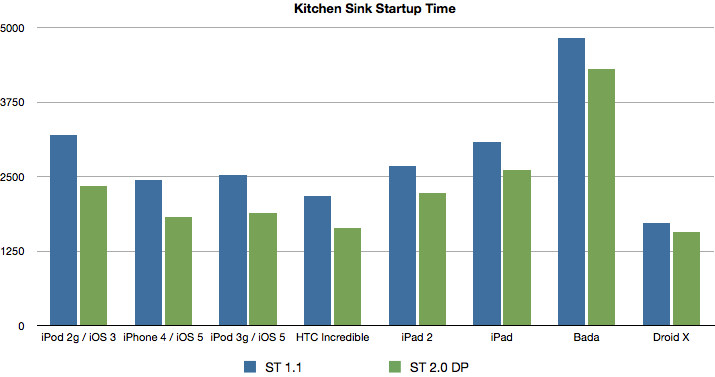
\includegraphics[width=0.8\textwidth]{figuren/sencha-touch-startup-times.png}
%   \caption{\st{} Kitchen Sink opstarttijden~\cite{SenchaInc.2013}.}
%   \label{fig:sencha_performance}
% \end{figure}

\paragraph{Aanpasbaarheid}
\label{sec:sencha-aanpasbaarheid}
Elke component binnen het raamwerk moet overerven van \code{Ext.Component}.  
Deze voorziet een attribuut \code{ui}.  
De waarde hiervan is een CSS-klasse die bepaald hoe de component er zal uitzien.  
\st{} heeft al twee CSS-klassen voorzien:  \code{light} en \code{dark}.  
Andere componenten kunnen deze lijst uitbreiden.  
Een knop kan bijvoorbeeld \code{normal},  \code{back},  \code{round},  \code{small},  \code{action} of \code{forward} als \code{ui} waarde hebben.

Het is ook mogelijk om eigen waarden voor \code{ui} te definiëren of de standaarden van \st{} aan te passen.  
SASS en Compass maken dit mogelijk door eigen CSS-bestanden aan te maken.  
SASS staat voor Syntactically Awesome Stylesheets en breidt CSS uit met variabelen,  geneste structuren, \term{mixins} en overerving~\cite{Eppstein2013}.  
\term{Mixins} groeperen enkele CSS-eigenschappen en kunnen worden hergebruikt.  
Compass is een raamwerk bovenop SASS en CSS.  
Het compileert SCSS (Sassy CSS) naar CSS-bestanden~\cite{Eppstein2013a}.        

\st{} thema's bestaan allemaal uit een set van \term{mixins}.  
Door zelf \term{mixins} te creëren of reeds bestaande te manipuleren kunnen eigen thema's gecreëerd worden en ze aan de \code{ui}-waarde van een component toegekend worden.

\paragraph{Programmeerbaarheid}
\label{sec:sencha-programeerbaarheid}
Zoals reeds aangehaald ondersteund \st{} het MVC-patroon.  
Dit patroon vermijdt lange \js{}-bestanden door ze logisch op te delen.  
Modellen groeperen velden tot een beschrijving van data-objecten, \code{Views} definiëren de weergave van componenten en controllers verbinden beide op basis van \term{events}.

In theorie zou het verschil tussen mobiele websites en applicaties enkel in de \code{Views} terug te vinden zijn.  
Echter,  dit wordt nog niet volledig ondersteund en worden aparte projecten voor deze functionaliteit gepromoot.

\paragraph{Ondersteuning browser}
\st{} steunt op de WebKit-browser \term{engine} dus moet de browser deze bevatten.  
Hoewel dit bij de meeste browsers geen probleem meer vormt, vallen toch enkele populaire browsers uit de boot.  
\st{} is bijvoorbeeld niet compatibel met FireFox Mobile en Opera Mobile~\cite{JohnEClark2012}.

Zoals reeds vermeld zijn er ook methoden voorzien om informatie op te vragen over de context die gehanteerd wordt (browser, OS, toestel, etc.).  
Verder kan \st{} ook vragen naar de ondersteuning van specifieke kenmerken (audio,  canvas,  CSS3, ...)  analoog als Modernizr.  

Op de Sencha website zijn voor de belangrijkste browsers en bijhorend besturingssystemen \term{scorecards} voorzien om hun compatibiliteit met HTLM5 en \st{} te bespreken~\cite{Inc.}.

%%%%%%%%%%%%%%%%%%%%%%%%%%%%%%%%%%%%%%%%%%%%%%%%%%%%%%%%%%%%%%%%%%
%%%%%%%%%%%%%%%%%%%%%%%%%%%%%%%%%%%%%%%%%%%%%%%%%%%%%%%%%%%%%%%%%%

\section{\kendo}
\label{sec:raamwerk-kendo}
\kendo{} is een raamwerk van de hand van Telerik.
Het bestaat uit drie luiken:  Web, Mobile en DataViz.  
Het eerste is gericht op de ontwikkeling van desktop- en mobiele applicaties,  het tweede voegt een \term{native look-and-feel} toe aan mobiele applicaties en het laatste zorgt voor datavisualisatie met HTML5- en \js{}-technologie.
\kendo{} is een \js{}-gedreven raamwerk met een MVVM-architectuur (zie infra) dat steunt op de jQuery bibliotheek.
Verder heeft de ontwikkelaar ook de mogelijkheid om eenvoudig de \term{backend} te integreren aan de klantzijde.
.NET,  PHP en JSP zijn momenteel de ondersteunde technologieën voor \term{backend} integratie.
Op het moment van schrijven is \kendo{} aan versie 2013 Q1~\cite{Telerik}. 

\subsection{Omkadering}
\label{sec:kendo-omkadering}

\paragraph{Programmeertaal}
\kendo{} kan zowel als \js{}- en opmaakgedreven beschouwd worden. 
Data-attributen in kunnen een HTML-element associëren met \kendo{} of het overeenkomstige jQuery object kan in \js{} het raamwerk oproepen en het element initialiseren.
Alle GI-elementen van \kendo{} Mobile kunnen met data-attributen worden opgebouwd.
\term{Widgets} van \kendo{} Web kunnen zowel met \js{} als data-attributen geïnitialiseerd worden.

Het laden van het raamwerk kan door heel \kendo{} op te roepen of enkel \kendo{} Mobile met respectievelijk \code{kendo.all.js} en \code{kendo.mobile.js}.
Elk van de drie luiken - Web, Mobile en DataViz - kan op zichzelf functioneren door hun \js{}-bestand in te laden.
Er kan wel slecht één van de drie script gelijktijdig gebruikt worden.  
Wanneer elementen uit verschillende luiken gebruikt worden, moet \code{kendo.all.js} worden gebruikt.
Een alternatieve oplossing is de keuze van het script van één luik en alle benodigde \js{}-bestanden te genereren met de \js{} Builder op \url{http://www.kendoui.com/custom-download.aspx}.
Hier kunnen de vereiste elementen geselecteerd worden en wordt het vereiste \js{}-bestand gegenereerd.
Op een analoge wijze als de \js{}-bestanden, kan de programmeur kiezen tussen verschillende \term{stylesheets}:  \code{kendo.all.css} en \code{kendo.mobile.css}.

\paragraph{Tools}
Op de \kendo{}-website staan drie webtools vermeld die Telerik aanbiedt om de programmeur te ondersteunen.
De eerste is \kendo{} Dojo~\cite{Telerika},  een interactieve leeromgeving om met \kendo{} vertrouwd te raken.
De gebruiker kan de basis van \kendo{} leren kennen met geleide handleidingen en uitvoerbare voorbeelden.
De twee andere webapplicaties zijn een ThemeBuilder voor Web en Mobile die op een grafische manier CSS-bestanden kunnen genereren~\cite{Telerikb,Telerikc}.
Voor \kendo{} Mobile kan een verschillende lay-out bepaald worden voor alle ondersteunde platformen.

\paragraph{Documentatie}
Alle documentatie kan gevonden worden op \url{http://docs.kendoui.com}~\cite{Telerikd}.
Twee belangrijke secties binnen de documentatie zijn de API en Getting Started.
Beide kunnen op elkaar gemapt worden omdat alle objecten van \kendo{} die in de API worden aangehaald ook in een pagina onder \term{Getting Started} worden besproken.
Deze laatste probeert met meer woorden en voorbeelden uit te leggen wat het object juist inhoudt.
Verder staan er bij de documentatie nog handleidingen die complexere functionaliteit uit de doeken doet.
Ook zijn er demo's die live voorbeelden tonen samen met de code die nodig is om het voorbeeld te maken.

\paragraph{Marktadoptatie}
Enkele van de populairste klanten van \kendo{} zijn Nikon,  Fujifilm en Symantec~\cite{Telerike}.

\paragraph{Licenties}
Een licentie voor \kendo{} Complete kost $\$699$ per ontwikkelaar.
Voor \term{backend} ondersteuning in PHP,  JSP of ASP.NET MVC moet $\$300$ meer betaald worden.
Hierbij zijn één jaar updates mogelijk en wordt professionele ondersteuning aangeboden met een responsetijd onder 48 uur.
Bij een licentie met \term{backend} integratie is support zelfs gegarandeerd na 24 uur.
Voor \kendo{} Web,  Mobile en DataViz bestaan ook een aparte licenties voor respectievelijk $\$399$,  $\$199$ en $\$399$~\cite{Telerik}.

\subsection{Code en ontwikkeling}
Zoals reeds vermeld moet de programmeur zowel \js{}- als HTML-code schrijven. 
De \js{}- en CSS-bestanden van het raamwerk moeten in de projectfolder worden gekopieerd respectievelijk in een \term{js}- en \term{styles}-map.
\kendo{} steunt op de jQuery-bibliotheek en deze moet ingeladen worden voor het \kendo{} raamwerk zelf wordt aangeroepen.
De initialisatie van een applicatie moet via \code{var app = new kendo.mobile.Application()}.
Hier kunnen parameters meegegeven worden die bijvoorbeeld de stijl van één platform vastlegt voor alle toestellen of het initiële scherm bepalen.

Net zoals bij \jqm{} zijn er drie strategieën om webapplicaties te maken:  volledige applicatie in één webpagina,  elk scherm in een aparte pagina of een combinatie van beide.
De navigatie naar een scherm gebeurt op basis van de \term{identifier} van dat scherm.
Standaard navigeert \kendo{} naar het eerste gedefinieerde scherm van een webpagina.
Een ander scherm kan in dezelfde pagina of in een ander bestand staan.
Een lokale navigatie wordt herkend door een \term{hashtag} die voor de id van het scherm wordt geplaatst als parameter van de \code{navigate}-methode.
Navigatie naar een ander bestand kan door de bestandsnaam als parameter op te geven.

\subsection{Functionele kenmerken}
\label{sec:kendo-functioneel}
%TODO klassensysteem
\kendo{} is zowel opmaak- als \js{}-gedreven en steunt op de MVVM-architectuur.
Dit beïnvloedt sterk alle functionele kenmerken.

\paragraph{UI-elementen}
Formulieren volgen de de HTML5-norm. 
Deze elementen zijn wel enkel functioneel op iOS 5.x en Android 4.x en hoger.  
Het stijl van de elementen op andere platformen zal werken, maar is beperkt tot  enkel tekstinvoer~\cite{Telerike}.

Het toevoegen van knoppen kan zowel met de \code{button}-tag als met standaard hyperlinks (\code{<a>}).
Knoppen kunnen ook samengevoegd worden tot een \code{ButtonGroup}.
Dit maakt het mogelijk om gemeenschappelijke acties aan een groep van knoppen toe te kennen om bijvoorbeeld een menu te maken.
Een \code{TabStrip} is een alternatief waar tabs in de voettekst het scherm kunnen laten variëren.

\paragraph{View}
Schermen worden voorgesteld met \code{Views},  analoog als bij de MVC-architectuur.
Een \code{View} aanduiden gebeurt door het attribuut \code{data-role} aan \code{View} gelijk te stellen.
\code{Views} kunnen met een lay-out worden voorzien met de \code{data-layout}-tag.
Een \code{Layout} bepaalt de vormgeving van een \code{View} en kan hergebruikt worden.

Een \code{ListView} is een specifieke \code{View} voor lijsten.
De \code{data-template} kan bij lijsten de \term{identifier} van een sjabloon bevatten die de opmaak van de lijstelementen definieert.
Deze sjablonen zijn specifieke \kendo{} scripts die HTML-tags en \js{}-code kunnen bevatten.
Ook kunnen ze verwijzen naar velden van het model dat aan de lijst is toegekend (zie infra).

Twee andere instanties van \code{Views} zijn \code{SplitView} en \code{ScrollView}.
De eerste kan het scherm in twee \code{Views} splitsen,  vaak gebruikt bij tabletapplicaties.
De tweede definieert een verzameling van pagina's die met een \term{swipe} bewegingen gelinkt zijn.

\paragraph{View-Model}
Het \code{View-Model} behoort tot de kern van \kendo{} en wordt \code{ObservableObject} genoemd.
Dit is een \js{}-object dat kan gebonden worden aan abonnees.
Het ondersteunt het monitoren van wijzigingen en verwittigt elke abonnee wanneer een wijziging zich voordoet.
Een \code{ObservableObject} kan aan een \code{View} worden toegekend door het in de \code{data-model}-tag te vermelden.

Er zijn verschillende bindingen	 mogelijk tussen een \code{View} en \code{ObservableObject}.
Deze wordt aangegeven in de \code{data-bind}-tag.
\kendo{} ondersteunt een binding met volgende eigenschappen:  \code{attr,  checked, clicked, custom, disabled, enabled, events, html, invisible, source, style, text, value} en \code{visible}.
Als een gebonden eigenschap wijzigt - door gebruikersinvoer of programmatisch - zal het overeenkomstige veld in het \code{ObservableObject} ook wijzigen.

\paragraph{Model}
Het \code{Model}-object erft over van \code{ObservableObject} en breidt het uit met de mogelijkheid om schema's,  velden en methoden te definiëren.  
Velden kunnen van het type \code{string, number, boolean} en \code{date} zijn.
Ook kunnen de velden verder beschreven worden door bijvoorbeeld een standaard waarde of validatie toe te voegen.
Een schema is een eigenschap van een \code{DataSource},  een \kendo{} object voor de opslag van lokale of externe data.  
Een \code{DataSource} ondersteunt alle CRUD (\term{Create, Read, Update en Delete}) operaties en het sorteren, pagineren, filteren, groeperen en aggregeren van data.
Het schema attribuut legt de structuur van de data in de \code{DataSource} vast.
Bij externe databronnen bepaalt het hoe binnenkomende data geparset moet worden om aan de opgelegde structuur te voldoen.
Een \code{Model} kan ook als waarde van het attribuut worden gezet.
Dit wil zeggen dat de bijhorende \code{DataSource} instanties zal bevatten van het toegekende \code{Model}.

\subsection{Niet-functionele kenmerken}
\label{sec:kendo-niet-functioneel}

\paragraph{Performantie}
De performantie van een \kendo{} applicatie wordt deels bepaald door de programmeur.
Deze moet er voor zorgen dat de data op het juiste moment geladen wordt.
Bij het weergeven van een \code{View} gaan drie gebeurtenissen vooraf,  namelijk \code{beforeShow,  init} en \code{show}.
De eerste wordt uitgevoerd voor een \code{View} zichtbaar wordt,  de tweede na initialisatie en de laatste bij het tonen van een \code{View}.
Het initialiseren van een \code{View} vindt maar één keer plaats nadat de volledige applicatie geladen is.
Bij de ontwikkeling van een \code{ListView} met data van een externe databron kan best de \code{DataSource} geladen worden bij het initialiseren van de applicatie,  de lijst gemaakt worden bij de \code{init}-gebeurtenis en de lijst ververst worden bij een \code{show}-gebeurtenis.

\paragraph{Aanpasbaarheid}
\kendo{} probeert de \term{native look-and-feel} van verschillende besturingssystemen na te bootsen.
%TODO Tim: deze zin uit Aanpasbaarheid en enkel bij Browserondersteuning.
%Op het moment van schrijven ondersteunt het iOS, Android, BlackBerry en Windows Phone~8.
Het \kendo{} pakket bevat ook tien extra thema's die een alternatieve lay-out bepalen.
Deze zijn elk nog persoonlijk aan te passen met de Mobile ThemeBuilder zoals beschreven in de sectie \ref{sec:kendo-omkadering}.

\paragraph{Programeerbaarheid}
\kendo{} is zowel JavaScipt- als opmaakgedreven.
Een kennis van zowel HTML als \js{} is vereist om met dit raamwerk aan de slag te kunnen.
Het raamwerk is gebouwd op de jQuery Core en maakt dus vaak van jQuery's \term{selectors} gebruik.
Ook kan een AJAX verzoek met jQuery syntax geformuleerd worden om externe data op te halen voor een \code{DataSource}.

\paragraph{Browserondersteuning}
Zoals reeds vermeld herkent \kendo{} het platform waarop de applicatie wordt uitgevoerd.
De lay-out van de applicatie zal de \term{native look-and-feel} van het besturingssysteem vervolgens nabootsen.
Ondersteunde systemen zijn iOS, Android, BlackBerry en Windows Phone~8.

Alle widgets, zoals gebruikt in het raamwerk, ondersteunen \term{progressive enhancement}.
Oudere browsers kunnen zo bestaande inhoud en functionaliteit raadplegen met \term{native} HTML-types indien bepaalde elementen niet worden ondersteund.
Ook de HTML5 formulierelementen worden opgebouwd met \term{progressive enhancement}.

%%%%%%%%%%%%%%%%%%%%%%%%%%%%%%%%%%%%%%%%%%%%%%%%%%%%%%%%%%%%%%%%%%
%%%%%%%%%%%%%%%%%%%%%%%%%%%%%%%%%%%%%%%%%%%%%%%%%%%%%%%%%%%%%%%%%%

\section{\jqm}
\label{sec:raamwerk-jqm}
\jqm{} is een opmaakgedreven raamwerk dat werd aangekondigd in 2010 en hoofdzakelijk gebruikersinterface-elementen (GI-elementen) aanbiedt~\cite{Resig2010}.
In november 2011 werd versie~1.0 uitgebracht~\cite{Parker2011} en een jaar later werd in oktober versie~1.2 uitgebracht~\cite{Parker2012}. 
Op het moment van schrijven zit \jqm{} aan versie~1.3.1~\cite{Parker2013b}. 
Het raamwerk wordt beheerd door het jQuery Project dat onder andere jQuery Core beheert en waar \jqm{} afhankelijk van is~\cite{JQuery2012}. 
\jqm{} wordt door onder andere Adobe, BlackBerry en Mozilla gesponsord~\cite{JQuery2012a}.

\subsection{Omkadering}
\paragraph{Programmeertaal}
Om met \jqm{} aan de slag te kunnen, is niets meer nodig dan kennis over HTML, CSS en \js{}. 
Alle GI-elementen worden geschreven in HTML en aangeduid met \code{data-}* attributen.

\paragraph{Tools}
Een standaard teksteditor voldoet om met \jqm{} aan de slag te kunnen. 
Natuurlijk kan het gemakkelijk zijn om van \term{integrated development environments}~(IDE's) zoals Aptana Studio~\cite{Aptana2012} of WebStorm~\cite{JetBrains2012} gebruik te maken, waardoor handige kenmerken zoals automatische code-aanvulling beschikbaar zijn.

Het is ook mogelijk om gebruik te maken van Codiqua om de GI-elementen op het scherm te slepen en neer te zetten. 
Codiqua zal automatisch op de achtergrond de HTML-code voorzien~\cite{Sperry2012}.

\paragraph{Documentatie}
Documentatie is te vinden op \exturl{www.jquerymobile.com/demos/1.2.0} voor versie~1.2. 
Hierop is een catalogus te vinden van alle mogelijke elementen waarover \jqm{} beschikt. 
Door de broncode van een voorbeeld te bekijken, kan worden gekeken welke code moet worden geschreven om tot dat resultaat te komen.

Naast de GI-elementen is er ook documentatie over de API. 
Deze gaat over initiële configuraties, \term{events} en methodes die kunnen worden gebruikt.

\paragraph{Marktadoptatie}
Op de website van \jqm{} wordt een reeks applicaties getoond die gemaakt zijn met hun raamwerk. 
Enkele voorbeelden zijn webapplicaties voor Ikea, Disney World, Stanford University en Moulin Rouge~\cite{JQuery2012a}. 

\paragraph{Licenties}
Sinds september 2012 is het enkel nog mogelijk om \jqm{} onder de Massachusetts Institute of Technology (MIT) licentie te verkrijgen~\cite{Dmethvin2012}. 
Dit betekent dat de code wordt vrijgegeven als \term{open-source} en dat deze tegelijkertijd kan worden gebruikt in propriëtaire projecten en applicaties~\cite{PhilDutson2012}.

\subsection{Code en ontwikkeling}
Zoals werd aangehaald, wordt voornamelijk HTML5-code geschreven voorzien van \code{data-}* attributen. 
Daarna zal het raamwerk door middel van \term{progressive enhancement} allerhande code toevoegen om de beoogde GI-elementen correct te tonen in de browser. 
Dit wordt verder uitgelegd in de sectie browserondersteuning (zie \ref{sec:jqm-browser-support}).

Er zijn drie strategieën om webapplicaties te maken in \jqm{}~\cite{Broulik2012}. 
Een eerste is om de volledige applicatie in één webpagina te schrijven. 
De vele schermen van de webapplicatie zijn dan allemaal samengebracht op eenzelfde webpagina. 
Het voordeel bij deze aanpak is dat er initieel minder verzoeken zijn naar de server omdat alles in één bestand wordt opgehaald. 
Dit geldt ook zo voor de geïmporteerde CSS- en \js{}-bestanden. 

Een tweede strategie is om voor ieder scherm een aparte webpagina aan te maken. 
Het voordeel hierbij is dat de eerste pagina waar de gebruiker op terecht komt, sneller wordt gedownload. 
Bij iedere navigatie naar een ander scherm, moet dit scherm via Asynchronous \js{} and XML~(AJAX) worden opgehaald, waardoor dit vertragend kan werken. 

Een laatste strategie is om een mix tussen beide te maken. 
Men kan bijvoorbeeld alle schermen die de gebruiker vaak nodig heeft op één webpagina plaatsen. 
De schermen die de gebruiker zelden nodig heeft, worden op aparte webpagina's geplaatst.   

\subsection{Functionele kenmerken}
\jqm{} is een raamwerk dat voornamelijk GI-elementen aanbiedt, met name pagina's en dialoogvensters, werkbalken, knoppen, inhoud vormgeven, elementen voor formulieren en lijsten~\cite{JQuery2012b}.
Deze kenmerken zijn gebaseerd op versie~1.2.

\begin{enumerate}
\item \textbf{Pagina's en dialoogvensters}
De basisstructuur van een pagina bestaat uit een koptekst, inhoud en voettekst. 
Bij het overgaan naar een andere pagina wordt gekozen uit tien overgangseffecten. 
Voordat deze overgang gebeurt, zal \jqm{} altijd eerst die pagina ophalen via AJAX en inladen in het DOM. 
Zo kan een soepel overgangseffect worden getoond aan de gebruiker. 
Daarnaast is het ook mogelijk om gelinkte pagina's op voorhand op te halen. 
Als laatste biedt \jqm{} ook dialoogvensters en pop-ups aan. 

\item \textbf{Werkbalken}
Het is mogelijk om zowel knoppen bij de koptekst als bij de voettekst te plaatsen. 
Bij deze laatste kunnen typisch meer knoppen geplaatst worden, bij de koptekst slechts twee. 
Daarnaast is het ook mogelijk om navigatiebalken te maken. 
Aan zowel de werk- als navigatiebalken kunnen iconen worden toegevoegd.

\item \textbf{Knoppen}
Het is ook mogelijk om knoppen te plaatsen in het inhoud gedeelde. 
Ook hier is er terug een variëteit aan mogelijkheden: grote of kleine, met iconen of zonder, gegroepeerd of niet. 

\item \textbf{Inhoud vormgeven}
De inhoud van de pagina kan worden vormgegeven door gebruik te maken van een rooster. 
\jqm{} laat roosters tot vijf kolommen toe. 
Daarnaast zijn er ook nog opklapbare blokken ter beschikking. 
Als laatste kunnen deze blokken ook samengevoegd worden tot een accordeon. 

\item \textbf{Elementen voor formulieren}
\jqm{} biedt alle gangbare elementen voor formulieren aan zoals tekstinvoer, een selectie uit een lijst, een zoekveld, een \term{slider} en een \term{switch}. 
Het raamwerk verplicht zelfs om de \code{<label>}-tag te gebruiken. 
Zo wordt de applicatie toegankelijker gemaakt voor bijvoorbeeld mensen met een \term{e-reader}.

\item \textbf{Lijsten}
Een laatste categorie GI-elementen die \jqm{} aanbiedt, zijn lijsten. 
Deze gaan van standaard ongeordende lijsten tot lijsten met alle soorten decoraties als iconen, afbeeldingen, telbubbels en verdelers. 
Ook is het mogelijk om in deze lijsten te zoeken. 
Hiervoor dient de gebruiker enkel één data attribuut toe te voegen, waarna het raamwerk de implementatie voorziet. 
\end{enumerate}

\subsection{Niet-functionele kenmerken}
\paragraph{Performantie}
Zoals gezegd schrijft de ontwikkelaar HTML5-code met specifieke data-attributen en zal het raamwerk daarna de code verder aanvullen. 
Dit gebeurt enkel op de pagina die de gebruiker op dat moment bekijkt. 
Dit gaat dus ook op voor een webapplicatie waarbij alle schermen op één webpagina zijn geschreven. 
Deze webpagina bevat allemaal \code{<div>}-verpakkingen voor ieder scherm. 
\jqm{} zal enkel die \code{<div>} verder aanvullen die op dat moment getoond wordt aan de gebruiker. 

\paragraph{Aanpasbaarheid}
Als \jqm{} \term{out-of-the-box} wordt gebruikt, zit alles goed qua kleur en design. 
Er is keuze uit vijf kleurenthema's die kunnen worden toegepast op de gehele applicatie of enkel op bepaalde elementen. 
Om een applicatie echt te laten onderscheiden van de andere, is een eigen kleurthema noodzakelijk. 
Hier is \jqm{} op voorzien door hun \term{stylesheet} op te delen in twee delen: thema's en structuur. 
Een ontwikkelaar kan ook enkel de structuur downloaden en zelf het thema in CSS schrijven. 
Doordat dit laatste heel wat inspanning vraagt, hebben de ontwikkelaars van \jqm{} ook een tool ter beschikking gesteld, namelijk ThemeRoller~\cite{JQuery2012c}. 
Hiermee worden de kleuren naar een voorbeeldapplicatie gesleept, waarna de overeenkomstige \term{stylesheet} kan worden gedownload.

\paragraph{Programmeerbaarheid}
Bij het programmeren in \jqm{} wordt geen enkel ontwerppatroon afgedwongen. 
De code voor de GI-elementen wordt tenslotte als HTML5-code geschreven. 
Voor de echte functionaliteit wordt beroep gedaan op \js{} en meer bepaald op de jQuery Core bibliotheek. 
Ook deze dwingt geen ontwerppatroon af.

\paragraph{Browserondersteuning}
\label{sec:jqm-browser-support}

% TODO Tim: verder uitwerken browser support
\jqm{} deelt browsers op in drie verschillende klassen: A, B en C~\cite{JQuery2012d}. 
Hierbij ondersteunt een klasse A browser alles, terwijl een klasse C browser enkel de basis HTML ondersteunt (en dus bijvoorbeeld geen hippe CCS3 overgangen).
\jqm{} maakt gebruikt van \emph{progressive enhancement} (zie \ref{par:progressive-enhancement}).
Hierdoor wordt in principe ieder apparaat ondersteunt door het raamwerk, maar zal de applicatie op een ouder apparaat minder functionaliteit krijgen dan diezelfde applicatie op een nieuw apparaat.

%%%%%%%%%%%%%%%%%%%%%%%%%%%%%%%%%%%%%%%%%%%%%%%%%%%%%%%%%%%%%%%%%%
%%%%%%%%%%%%%%%%%%%%%%%%%%%%%%%%%%%%%%%%%%%%%%%%%%%%%%%%%%%%%%%%%%

%TODO: verder uitschrijven, maar dat zal blijken uit mijn implementatie
\section{\lungo}
\label{sec:raamwerk-lungo}
\lungo{} is een opmaakgedreven raamwerk waarbij versie~1.0 uitkwam in 2011~\cite{TapQuo2011}.
Het raamwerk wordt onderhouden door TapQuo dat een Spaans bedrijf is, gespecialiseerd rond mobiele gebruikerservaring~\cite{TapQuo2013a}.
\lungo{} is afhankelijk van een \js{}-bibliotheek, namelijk \quo{}.
\lungo{} biedt vooral GI-elementen aan, maar daarnaast zijn er ook \term{wrappers} voor cache, opslag en SQL beschikbaar~\cite{TapQuo2013}.
Er wordt geen programmeerstijl zoals MVC afgedwongen.
Op het moment van schrijven zit \lungo{} aan versie~2.1~\cite{TapQuo2013}.

\subsection{Omkadering}
\paragraph{Programmeertaal}
Er is niets meer nodig dan kennis over HTML, CSS en \js{}.
De GI-elementen worden geschreven in HTML en aangeduid aan de hand van CSS-klassen en \code{data-*}-attributen

\paragraph{Tools}
Er worden geen specifieke tools door TapQuo aangeboden om de ontwikkeling te versnellen.
Wel kan er gebruik worden gemaakt van Twitter Bower die helpt om de bestanden van het \lungo{}-raamwerk tezamen met de \quo{}-bibliotheek te beheren~\cite{Twitter2013}.
%TODO Tim: verplaatsen naar uitleg bij evaluatie
%Dit is bij \jqm{} niet mogelijk doordat \jqm{} geen geldige component is van Bower.

\paragraph{Documentatie}
De documentatie begint op \exturl{lungo.tapquo.com/howto/prototype/} waar getoond wordt hoe het geraamte van een typische \lungo{}-applicatie er uitziet.
Vervolgens zijn er nog acht andere hoofdstukken die de aangeboden GI-elementen en API uitleggen.
Op de documentatiepagina's is altijd eerst de broncode te zien.
Er kan dan boven de broncode op een knop geklikt worden, waarna een livevoorbeeld wordt getoond.

\paragraph{Marktadoptatie}
%TODO Tim: mail gestuurd

\paragraph{Licenties}
Het raamwerk wordt onder de GPLv3-licentie vrijgegeven.
%TODO Sander: ik ben geen licentie expert,  wat is het verschil tussen gplv3 en commercieel?  Mss iets uitwerken?
%Tim: zoals toen vrijdag verteld heb ik ook hiervoor een mail gestuurd
Een commerciële versie is mogelijk.

\subsection{Code en ontwikkeling}
Zoals gezegd wordt een \lungo{}-applicatie geprogrammeerd vanuit geannoteerde HTML-code door middel van CSS-klassen.
Er wordt geen programmeerstijl zoals MVC afgedwongen.

Om de verschillende schermen te scheiden wordt gebruik gemaakt van \code{<article>}- en \code{<section>}-tags die specifiek zijn voor HTML5.
Analoog wordt ook voor de kop- en voettekst de \code{<header>}- en \code{<footer>}-tags gebruikt.
%TODO Tim: verplaatsen naar evaluatie
%Hierdoor is het duidelijk dat \lungo{} ten opzichte van \jqm{} volledig gebruik maakt van de nieuwste HTML5-tags.

\lungo{} biedt de mogelijkheid om de verschillende schermen op afzonderlijke pagina's op te slaan en daarna asynchroon op te halen.
%TODO Tim: verplaatsen naar evaluatie
%In tegenstelling tot \jqm{} dient enkel wat binnen de \code{<body>}-tag staat, opgeslaan te worden.
%Bij \jqm{} dient telkens ook de volledige \code{<head>}-tag op iedere pagina herhaald te worden.

\subsection{Functionele kenmerken}
De documentatiepagina is opgedeeld in negen groepen die hieronder kort worden aangehaald.

\begin{enumerate}

\item \textbf{Prototype } 
Hierop worden GI-elementen, navigatie, formulieren, scrollen, lijsten en data-attributen aangehaald. 
Opmerkelijk is de directe ondersteuning door het raamwerk bij het naar beneden trekken van een lijst waarbij de data automatisch wordt herladen.

\item \textbf{Core }
Hier worden functies aangehaald die het raamwerk zelf intern gebruikt.
Een voorbeeld hiervan is de \code{Lungo.Core.isMobile()}-functie die controleert of de applicatie in een mobiele omgeving wordt uitgevoerd.

\item \textbf{Data }
Zoals aangehaald in de inleiding biedt het raamwerk \term{wrappers} voor cache, opslag en SQL.
De ontwikkelaar dient dus zelf geen \code{if-then-else}-constructies op te stellen of een bepaald kenmerk ondersteund wordt of niet, het raamwerk neemt dat voor zijn rekening.

\item \textbf{DOM }
Het manipuleren van de DOM gebeurt door de \quo{}-bibliotheek.
Hiervoor wordt gerefereerd naar de documentatie op \exturl{quojs.tapquo.com}.

\item \textbf{Element }
Toevoegen van een telbubbel, vooruitgangsbalk, laadbalk, automatisch herladen bij het naar beneden trekken van lijst en een fotocarousel zijn mogelijk vanuit \js{}. 

\item \textbf{Notification }
Er worden standaard verschillende dialoogvensters aangeboden voor fout-, succes- en infomeldingen.
 
\item \textbf{Routing }
Hier wordt uitgebreid ingegaan op de navigatie doorheen de applicatie vanuit \js{}.

\item \textbf{Service }
Versturen van HTTP-oproepen kan zonder meer vanuit het \lungo{}—raamwerk.

\item \textbf{View }
Hier worden \js{}-methoden aangeboden om het uitzicht binnen een \code{<article>} te bepalen.
 
\end{enumerate}

\subsection{Niet-functionele kenmerken}
\paragraph{Performantie}
De \js{}-bibliotheek waarop \lungo{} steunt is geoptimaliseerd voor mobiel gebruik.
Hierdoor bevat het geen methodes voor desktopgebruikers, waardoor het bestand kleiner is dan traditionele \js{}-bibliotheken.

\paragraph{Aanpasbaarheid}
\label{sec:lungo-aanpasbaarheid}
Standaard zit een \lungo{}-applicatie goed qua lay-out.
TapQuo biedt zelf geen tools aan om de kleuren of het uitzicht van de applicatie te veranderen.
Hierdoor zal een ontwikkelaar zelf aangewezen zijn om eigen CSS-code te schrijven.

\paragraph{Programmeerbaarheid}
\label{sec:lungo-programeerbaarheid}
\lungo{} dwingt geen enkel ontwerppatroon af.
Voor de echte functionaliteit wordt beroep gedaan op \js{} en meer bepaald op \quo{}. 
Ook deze dwingt geen ontwerppatroon af.

\paragraph{Ondersteuning browser}
TapQuo geeft aan op hun website dat ze ondersteuning bieden voor iOS, Android, Blackberry en FirefoxOS.
Verder halen ze aan dat ze een zelfde ervaring willen hebben voor een gemaakte applicatie gaande van mobiele apparaten, tv's tot desktopapparaten.

%%%%%%%%%%%%%%%%%%%%%%%%%%%%%%%%%%%%%%%%%%%%%%%%%%%%%%%%%%%%%%%%%%
%%%%%%%%%%%%%%%%%%%%%%%%%%%%%%%%%%%%%%%%%%%%%%%%%%%%%%%%%%%%%%%%%%

\section{Tabel}
\label{sec:raamwerken-tabel}

In tabel~\ref{tabel:raamwerken-tabel} wordt de vergelijking van de raamwerken getooond op basis van passieve vergelijkingscriteria.
Dit is een vergelijking gebaseerd op informatie van de raamwerken die hiervoor kan worden teruggevonden.
De passieve vergelijkingscriteria vergelijken de raamwerken met gevonden informatie over het raamwerk zelf.
De data is samengezet,  geen extra onderzoek werd verricht.
In het volgende hoofdstuk worden vijf actieve vergelijkingscriteria besproken.
Deze zijn actief onderzocht en de resultaten hiervan zullen in hoofdstuk \ref{chap:evaluatie} besproken worden.

\begin{landscape}
\begin{table}[H]
\centering
\pgfplotstabletypeset[
  begin table=\begin{tabular}{p{5cm} p{3.5cm} p{3.5cm} p{3.5cm} p{3.5cm}},
  end table=\end{tabular},
  col sep=comma,
  string type,
  header=true,
  skip coltypes=true,
  columns={Criterium,ST,Kendo,jQM,Lungo},
  columns/Criterium/.style={column name=\textbf{Criterium}},  
  columns/jQM/.style={column name=\textbf{\jqm}},
  columns/ST/.style={column name=\textbf{\st}},
  columns/Kendo/.style={column name=\textbf{\kendo}},
  columns/Lungo/.style={column name=\textbf{\lungo}},
  every head row/.style={
    before row=\toprule,
    after row=\midrule},
  every last row/.style={
    after row=\bottomrule}
]{tabellen/raamwerken.csv}
%TODO Tim: dit is hier de eerste keer dat de term 'passieve vergelijkingscriteria' valt, dus dat moet er voor nog eens goed uitgelegd worden
\caption{Samenvattende tabel voor passieve vergelijkingscriteria van mobiele HTML5-raamwerken}
\label{tabel:raamwerken-tabel}
\end{table}
\end{landscape}

\chapter{Vergelijkingscriteria}
\label{chap:vergelijkingscriteria}

Dit hoofdstuk bekijkt hoe de mobiele HTML5 raamwerken actief zullen worden vergeleken.
Hoofdzakelijk zal dit gebeuren aan de hand van een \term{proof of concept}~(POC).
Deze wordt geïntroduceerd in sectie \ref{sec:vergelijking-poc} en zal hoofdzakelijk de gekozen vergelijkingscriteria in sectie \ref{sec:vergelijking-criteria} drijven.
De criteria die worden voorgesteld, zullen voortaan actieve criteria worden genoemd.


\section{POC}
\label{sec:vergelijking-poc}
In samenspraak met Capgemini werd gekozen om een \term{proof of concept}~(POC) op te stellen.
%TODO hier refereren en reflecteren over POC in literatuur
Dit is een idee waarbij de uitvoerbaarheid in de verschillende raamwerken kan worden nagegaan.
Verschillende vergaderingen werden georganiseerd om tot een idee te komen dat vooral in de bedrijfswereld van toepassing is.
Het uiteindelijke idee is een applicatie die het mogelijk maakt voor werknemers om hun onkosten via hun mobiel apparaat door te sturen.

Het idee werd uitgewerkt door Capgemini en geleverd aan de auteurs als \term{mockup}.
Dit is een voorstelling van de applicatie als een reeks schermen zoals deze er zullen uitzien op een apparaat. 
Een voorbeeld van zo een scherm is te vinden op figuur~\ref{fig:poc}. 
Naast de schermen staan de functionele vereisten die op het scherm van toepassing zijn.
De bedoeling is dat deze POC wordt uitgewerkt zowel voor smartphone als tablet, zowel voor Android als iOS, zowel voor staande als liggende apparaten en zowel voor online als offline gebruik.

\begin{figure}
  \centering
  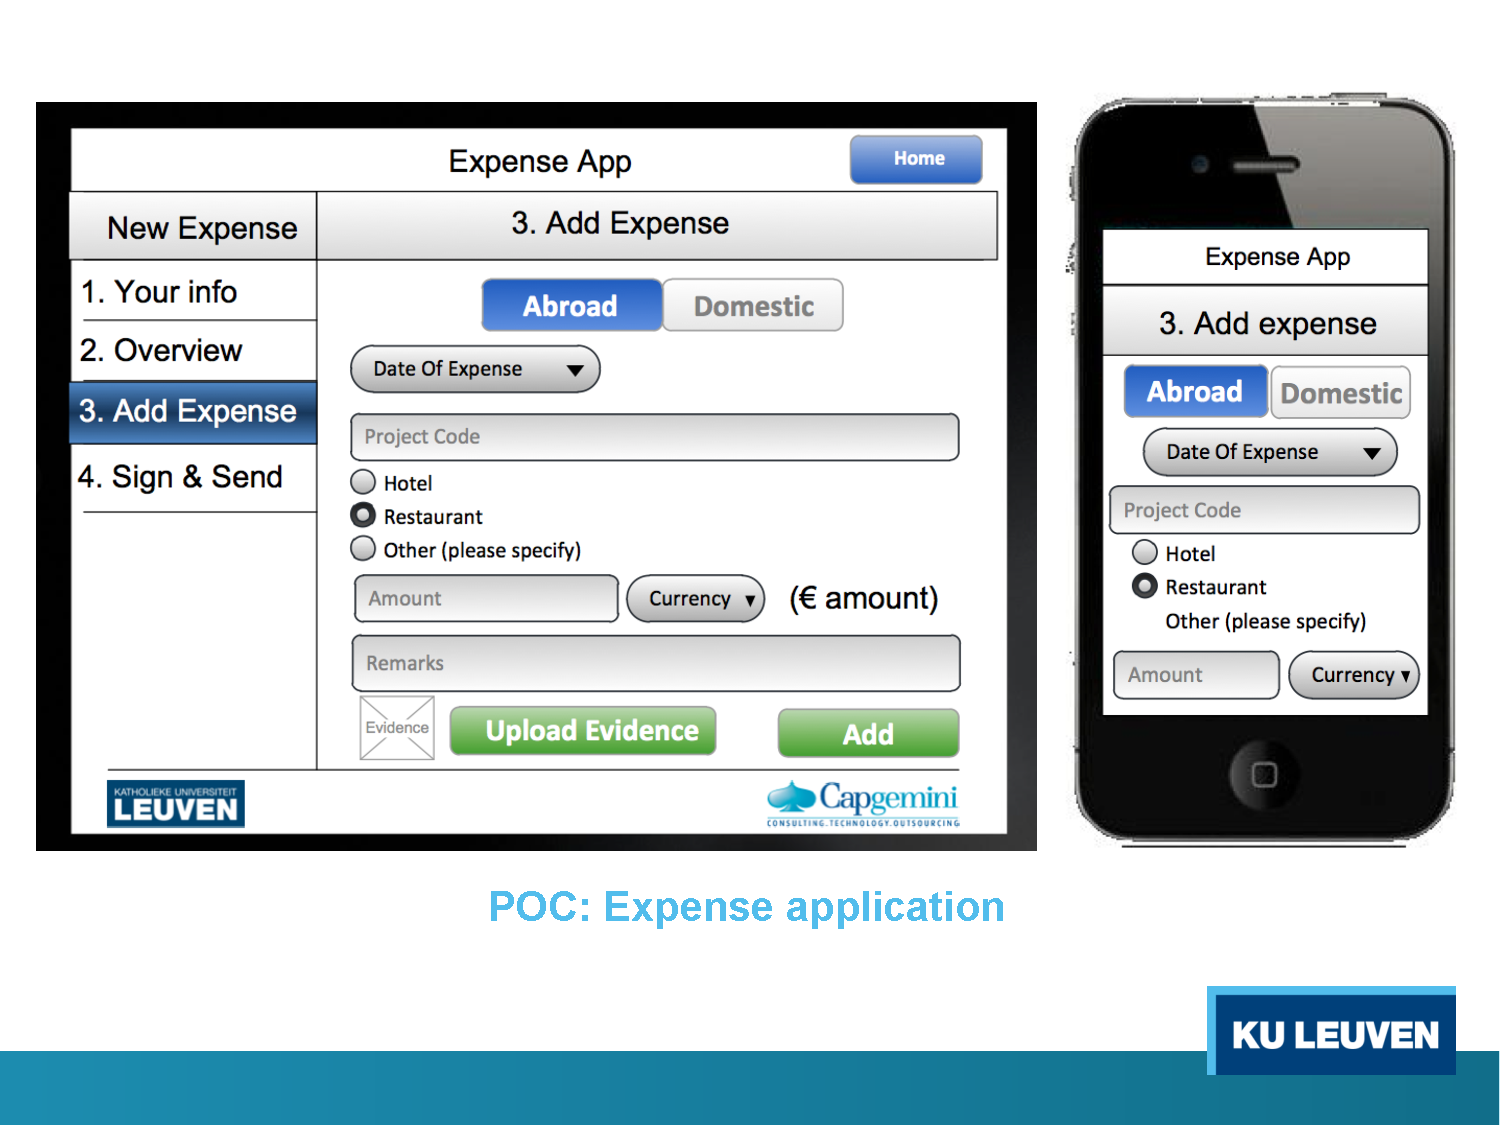
\includegraphics[trim=0cm 4.6cm 0cm 1.55cm,clip=true,width=\textwidth]{figuren/poc.pdf}
  \caption{POC bij het toevoegen van een nieuwe onkost met aan de linkerkant de weergave op een tablet en aan de rechterkant deze op een smartphone.}
  \label{fig:poc}
\end{figure}

\subsection{Aspecten}
\label{sec:vergelijking-poc-detail}

Een werknemer meldt zich eerst aan op de applicatie en kan daarna ofwel een nieuw onkostenformulier aanmaken of zijn doorgestuurde onkostenformulieren bekijken.
De term onkostenformulier is een groepering van meerdere onkosten met bijhorende bewijsstukken en de handtekening van de werknemer. 
Het aanmaken van een nieuw onkostenformulier verloopt in vier stappen.
Indien de werknemer al eerder begonnen was met het aanmaken van een formulier, zal hij worden gevraagd of hij verder wil gaan met dat formulier of met een nieuw formulier wil starten.

\begin{enumerate}
\item De eerste stap is het bekijken en/of aanpassen van de persoonlijke informatie van de werknemer.
Bij het aanpassen van deze gegevens, zullen deze worden gevalideerd.
Indien deze validatie faalt, krijg de werknemer een dialoogvenster te zien met de reden tot falen.
Ook worden de foute velden rood gemarkeerd.

\item In de tweede stap kan de werknemer zijn toegevoegde onkosten aan het formulier bekijken.
In het begin is deze lijst leeg, tenzij hij eerder een formulier aan het invullen was (zie infra).
Indien deze lijst onkosten bevat, is het mogelijk om hierop te klikken en deze te bekijken.
Aanpassen is niet mogelijk.

\item In stap drie kan een nieuwe onkost worden toegevoegd.
Dit kan ofwel een binnenlandse ofwel buitenlandse onkost zijn.
Voor beide dient een datum en projectcode te worden opgegeven.
De eerstgenoemde is een \term{datepicker} die teruggaat tot twee maanden in de tijd.
De laatstgenoemde bevat automatische aanvulling, maar de werknemer is niet verplicht om een projectcode uit de aanvulling te selecteren.
Daarnaast dient het type en bedrag van de onkost, alsook een bewijsstuk te worden opgegeven.
Bij een buitenlandse onkost moet de munteenheid worden opgegeven, waarna de applicatie deze automatisch omvormt naar euro.
Het scherm voor het toevoegen van een buitenlandse onkost wordt getoond op figuur \ref{fig:poc}. 
Net zoals bij stap één geldt ook hier validatie op de formuliervelden.

\item In deze laatste stap dient een handtekening te worden geplaatst waarna het formulier kan worden doorgestuurd.
Indien de gebruiker offline werkt, zal deze worden opgeslagen op het toestel.
De werknemer kan het formulier opnieuw doorsturen zodra hij terug online is.

\end{enumerate}

Bij het bekijken van de doorgestuurde formulieren is het mogelijk om per formulier de bijhorende PDF te downloaden. 
Deze bevat een overzicht van de onkosten met bijhorende bewijsstukken, alsook de handtekening van de werknemer.

\section{Criteria}
\label{sec:vergelijking-criteria}

In deze sectie zullen de actieve criteria toegelicht worden die zullen worden toegepast om de raamwerken te vergelijken.
In sectie \ref{sec:vergelijken-raamwerken} werden reeds technieken besproken die in de literatuur worden toegepast.
Elementen van deze technieken zullen terugkomen in de voorgestelde methode om de raamwerken te evalueren.
%TODO in elke sectie van een criteria een referentie naar literatuur (zie drive document) + reflecteren met ISO
Sectie \ref{sec:raamwerken-tabel} bevatte de passieve vergelijkingscriteria die raamwerken vergeleken met informatie over het raamwerk zelf.

Vijf criteria zullen worden gebruikt: populariteit (\ref{sec:vergelijking-populariteit}), productiviteit (\ref{sec:vergelijking-productiviteit}), gebruik (\ref{sec:vergelijking-gebruik}), ondersteuning (\ref{sec:vergelijking-ondersteuning}) en performantie (\ref{sec:vergelijking-performantie}). 
%TODO refereren naar puntensysteem literatuur + AHP gewichten zijn voor alle criteria gelijk
Elk raamwerk krijgt voor elk criterium een score afgeleid uit een formule. 
Deze scores zullen in een spinnenweb worden ondergebracht (zie sectie \ref{sec:vergelijking-spinnenweb}).
Zoals hierboven vermeld zal een POC gebruikt worden bij de vergelijking.
%TODO productiviteit laten vallen?  Laatste zin?
De implementatie van deze POC zal het productiviteits-, gebruiks- en ondersteuningscriterium drijven.  
Dit komt omdat Capgemini de POC zo heeft opgesteld dat het de verschillende functionaliteiten bevat die van een normale applicatie verwacht worden.
Zo is de POC representatief om een volledige vergelijking te kunnen maken.

\subsection{Populariteit}
\label{sec:vergelijking-populariteit}
%TODO populariteit is een factor voor de gemeenschap en ``levendigheid'' van het raamwerk
De populariteit van een raamwerk kan in cijfers worden uitgedrukt door gebruik te maken van sociale netwerken. 
Een tabel zal voorzien worden met in de rijen het aantal volgers op Twitter, sterren en \term{forkers} van \gh{},  vragen op \so{} en aantal vind-ik-leuks van \fb{}~\cite{Sarrafi2012a,Ayuso2012}. 

GitHub kan worden gezien als een sociaal netwerk voor programmeurs~\cite{Catone2008} en bepaalt dus de actieve gemeenschap rond het raamwerk.
Raamwerken die niet op GitHub te vinden zijn krijgen nul voor zowel het aantal sterren en \term{forkers}.
Een alternatief hield de interpolatie van de GitHub data van de overige raamwerken in.
Omdat deze aanpak het raamwerk onterecht zou bevoordelen, is hier niet voor gekozen.

De som van Twitter volgers ($T_r$), \gh{} sterren ($S_r$), \gh{} \term{forkers} ($F_r$), \so{} vragen ($SO_r$) en \fb{} vind-ik-leuks ($FB_r$) vormt de score voor het populariteitscriterium:
\begin{equation}
  \text{Populariteit}_r=T_r+S_r+F_r+SO_r+FB_r
  \label{eq:populariteit}
\end{equation}
voor een raamwerk $r$.

%TODO als figuur in evaluatie wordt weggelaten, ook deze zin
Omdat deze gegevens zeer dynamisch zijn, zullen verschillende metingen in de tijd de evolutie van de data weergeven.
Ook zullen de uitkomsten van dit criterium worden vergeleken met data geleverd door Google Trends~\cite{Google2012a}.
Deze webapplicatie toont de evolutie van zoektermen op Google op een schaal van 100, waarbij 100 overeenkomt met de grootste zoekinteresse.
Voor elk raamwerk zal het aantal zoekopdrachten op Google in functie van de tijd worden uitgezet.

Er bestaat geen exacte formule om populariteit uit te drukken.
De formule die werd gekozen om de score voor dit criterium te quoteren is onderheven aan subjectiviteit.
Twee opmerkingen moeten hierbij worden gemaakt.
Enerzijds zijn de auteurs zich ervan bewust dat de doorsnede tussen sociale netwerken niet leeg is.
Zo kan éénzelfde persoon zowel een volger op Twitter zijn als een vind-ik-leuk op \fb{} plaatsen.
Verschillende individuen zullen dus dubbel geteld worden in de totale score voor populariteit van het raamwerk.
De score zal dus slechts een indicatie geven over de populariteit,  het is geen exacte weergave.
Ten tweede zijn de auteurs er zicht van bewust dat de inclusie van \so{} op twee manieren kan worden bekeken.
Enerzijds kunnen veel vragen duiden op veel onduidelijkheden over het raamwerk.
Anderzijds kan dit een maat zijn voor de populariteit van dit onderwerp.
De auteurs zijn van mening dat de tweede zienswijze correcter is dan de eerste en het dus valide is \so{} in de formule op te nemen.

%%%%%%%%%%%%%%%%%%%%%%%%%%%%%%%%%%%%%%%%%%%%%%%%%%%%%%%%%%%%%%%%%%
%%%%%%%%%%%%%%%%%%%%%%%%%%%%%%%%%%%%%%%%%%%%%%%%%%%%%%%%%%%%%%%%%%

\subsection{Productiviteit}
\label{sec:vergelijking-productiviteit}
Hoe lang het duurt om met het raamwerk vertrouwd te raken en iets nuttig te kunnen bouwen kan met productiviteit berekend worden.
%TODO time is money (minder is beter)
%TODO deze zin weglaten?
De auteurs zullen het raamwerk testen met een implementatie van de POC.
%TODO wel verschillende mensen !
Er wordt verondersteld dat de auteurs over een gemeenschappelijke technische achtergrond beschikken.

Elk zullen ze de POC in twee verschillende raamwerken maken en daarnaast ook een extra loginapplicatie in twee andere raamwerken.
De ene auteur maakt de POC in \jqm{} en \lungo{} en de loginapplicatie in \st{} en \kendo{}.
De andere zal dan de POC in \st{} en \kendo{} maken en de loginapplicatie in \jqm{} en \lungo{}.
De tijd die nodig is om de volledige POC te implementeren is een indicatie voor de productiviteit. 

% Omdat de POC twee keer moet worden geïmplementeerd, wordt verwacht dat de tweede implementatie sneller zal verlopen.
% Dit probleem is onafwendbaar en zal bij de evaluatie van de data aangehaald worden.
% De uren voor de implementatie van de loginapplicatie zal de score correcter maken.
% 
% De som van de uren voor het implementeren van de POC ($t_{r,POC}$) en de loginapplicatie ($t_{r,login}$) vormt de score voor de productiviteit:
% \begin{equation}
%   \text{Productiviteit}_r = {t_{r,POC} + t_{r,login}}
%   \label{eq:productiviteit}
% \end{equation}
% voor een raamwerk $r$.

%TODO Sander verleden tijd of tt tijd schrijven?  Het zijn onze persoonlijke bevindingen na de implementatie dus vt?
Er zijn echter vijf redenen waarom de implementaties van de POC geen goede indicatie zijn voor de productivteit.
Deze werden door de auteurs bevonden wanneer de implementatie in het tweede raamwerk werd uitgevoerd:
\begin{enumerate}
\item Betere ervaring met de POC versnelt bij de tweede implementatie het overzicht van vereisten die moeten worden geïmplementeerd. 
\item Een verbeterde ervaring met HTML5-raamwerken had een positieve invloed op de verdere implementaties.
Dit weerspiegelde zich vooral tussen \jqm{} en \lungo{}.
Hoewel ze beide op een verschillende \js{}-bibliotheek steunen - respectievelijk jQuery en QuoJS - zijn de gelijkenissen tussen deze twee raamwerken groot.
Ook leggen ze beide geen architectuur op.
\item Er kon code,  zoals van de implementatie in \jqm{},  overgenomen worden bij de implementatie van de POC met \lungo{} en \kendo{}.
\item Er kwamen bij de eerste implementatie problemen met de \term{backend} naar boven.
Deze waren bij de tweede implementatie reeds opgelost.
Door het onnauwkeurig opmeten van de tijd kan er geen schatting worden gemaakt van de tijd die aan de problemen van de \term{backend} werden besteed.
\item Niet de volledige POC kon met \lungo{} en \st{} worden ontwikkeld.
\end{enumerate}

De implementatie van de loginapplicatie is een alternatieve test van de productiviteit.
Deze applicatie bevat GI-elementen, validaties,  \term{backend} integratie en een lijst.
De implementatie van de loginapplicatie kan dus als voldoende steekproef beschouwd worden om ervaring met een raamwerk te testen.
Na het aanmelden met deze applicatie zal de gebruiker een lijst van $850$ elementen te zien krijgen.
Deze lijst is bedoeld als stresstest om de performantie te testen (zie sectie \ref{sec:vergelijking-performantie}).
De elementen in de lijst zullen voorzien worden van een afbeelding en tekst.
De lijst kan als een potentiële muziekapplicatie gezien worden waarbij de afbeelding en tekst naar liedjes verwijzen.
Het aantal elementen in de lijst - $850$ - is een schatting van het maximum aantal liedjes dat ooit is opgenomen~\cite{Zimmy2011}.
Het kan dus als bovengrens voor dit soort applicaties worden beschouwd.
De implementatie van deze applicatie zal een indicatie geven hoe snel,  zonder al te veel voorkennis van het raamwerk,  één eenvoudige applicatie opgeleverd kan worden.

% De werkuren van de loginapplicatie bevestigen voorgaande resultaten niet.
De werkuren van de loginapplicatie bleken niet onderheven aan de vijf zonet opgenoemde tegenargumenten:
\begin{enumerate}
\item Bij elke implementatie werd met dezelfde achtergrondkennis gestart.  
De implementatie van de loginapplicatie is triviaal en eenduidig.
Er geldt dus voor alle raamwerken dat de ervaring met de applicatie reeds hoog was.
\item Eerst werd de implementatie van de POC gemaakt voordat aan de loginapplicatie werd begonnen.
Hierdoor was de algemene ervaring met HTML5-raamwerken reeds groot.
\item Er werd geen code gekopieerd. 
\item Er waren geen problemen met de \term{backend}.
\item Alle functionaliteit van de loginapplicatie kon met alle vier raamwerken worden gebouwd.
\end{enumerate}
Om al deze redenen werd beslist de score voor productiviteit te bepalen door enkel de uren van de login applicatie ($t_{r,login}$) te beschouwen.
De formule voor productiviteit is dan:
\begin{equation}
  \text{Productiviteit}_r = t_{r,login}
  \label{eq:productiviteit-enhanced}
\end{equation}
voor een raamwerk $r$.

De uitkomsten van dit criterium zullen gestaafd worden door het aantal lijnen code te presenteren die nodig waren voor zowel de POC als de loginapplicatie te bouwen.
Ook zullen de factoren die de leercurve bepalen, worden bekeken. 
Dit zijn ten eerste de tools die de programmeur kan gebruiken om eenvoudiger te ontwikkelen.
Vervolgens zal de kwaliteit en kwantiteit van de documentatie van elk raamwerk worden bekeken.
De mogelijkheden voor debuggen bepalen ook de leercurve en zullen worden onderzocht.
Tot slot zal gekeken worden naar de aanwezige literatuur van het raamwerk en waar ontwikkelaars met vragen terecht kunnen.

%%%%%%%%%%%%%%%%%%%%%%%%%%%%%%%%%%%%%%%%%%%%%%%%%%%%%%%%%%%%%%%%%%
%%%%%%%%%%%%%%%%%%%%%%%%%%%%%%%%%%%%%%%%%%%%%%%%%%%%%%%%%%%%%%%%%%

\subsection{Gebruik}
\label{sec:vergelijking-gebruik}
%TODO zoveel mogelijk features of plug-ins van een raamwerk zijn belangrijk want dan kan je meer met een raamwerk doen
Uit de \term{mockup} schermen en de bijhorende functionele vereisten werden $13$ uitdagingen met in totaal $38$ deeluitdagingen geëxtraheerd.
Alle functionaliteit die potentieel door een raamwerk kan worden geleverd en in de POC wordt gebruikt, zit in een uitdaging vervat.  
Echter, een voorbeeld van functionaliteit van de POC die niet in een uitdaging zit, is de omzetting van \term{identifiers} naar een tekstuele vorm.
Dit is geen interessante functionaliteit omdat het eigen is aan de POC zelf.
De implementatie hiervan zal uitsluitend uit \js{}-code bestaan.
Alle uitdagingen en deeluitdagingen zijn in tabel~\ref{tabel:uitdagingen} te vinden.

\pgfplotstabletypeset[
  begin table=\begin{longtable}{l},
  end table=\caption{$13$ uitdagingen onderverdeeld in $38$ deeluitdagingen voor gebruik.}\label{tabel:uitdagingen}\end{longtable},
  skip coltypes=true,
  col sep=comma,
  string type,
  header=true,
  columns={Uitdaging},
  columns/Uitdaging/.style={column name=\textbf{Uitdagingen}, column type={l}},  
  every head row/.style={
    before row=\toprule,
    after row=\midrule},
  every last row/.style={
    after row=\bottomrule}
]{tabellen/uitdagingen.csv}

De wijze waarop het raamwerk de uitdaging aangaat zal de score bepalen.
Er onderscheiden zich drie gevallen.
De hoogste score ($2$) wordt toegekend wanneer de functionaliteit aangeboden wordt door het raamwerk. 
Een lagere score ($1$) betekent dat een plug-in moet worden gezocht.
Omdat de raamwerken bouwen op HTML5, zal een kenmerk van HTML5 ook als plug-in beschouwd worden.
Voor een oplijsting van de HTML5 kenmerken wordt naar sectie \ref{sec:html5-css3-js} verwezen.
Wanneer de implementatie zelf moet worden geschreven of een hack noodzakelijk is, zal de laagste score ($0$) worden toegekend.
Ook is het mogelijk  dat de uitdaging helemaal niet wordt geïmplementeerd.
Dit is mogelijk wanneer het raamwerk de functionaliteit niet ondersteund,  geen plug-in werd gevonden en niet aan een eigen implementatie wordt begonnen.
Dit zal leiden tot een $0$ score.
Wanneer CSS-code wordt gebruikt om de uitdaging te implementeren, zal de laagste score worden toegekend.
Het gebruik van CSS3 wordt echter als kenmerk van HTML5 gezien en vervolgens met $1$ gequoteerd.

Tabel \ref{tabel:scores-uitdagingen} toont de mogelijke scores $U_{r,i}$ van raamwerk $r$ en voor uitdaging $i$.
\begin{table}	
  \centering
  \begin{tabular}{ll}
    \toprule
    \textbf{Score} & \textbf{Verklaring}\\
    \midrule
    $U_{r,i} = 2$ & Ondersteund door het raamwerk\\
    $U_{r,i} = 1$ & Een plug-in of kenmerk van HTML5 is nodig\\
    $U_{r,i} = 0$ & Eigen implementatie of hack of niet geïmplementeerd\\ 
    \bottomrule
  \end{tabular}
  \caption{Beoordeling uitdagingen gebruikscriterium}
  \label{tabel:scores-uitdagingen}
\end{table}

De potentiële score van een uitdaging is discreet en ligt tussen $0$ en $2$.
Er zijn dus slechts $3$ scores waaruit gekozen kan worden om de implementatie te beoordelen.
De verklaringen bij de scores omvatten alle gevallen op een eenduidige manier.
Een alternatief bestaat uit $4$ scores waarbij HTML5-kenmerken een lagere score krijgen ten opzichte van plug-ins.
Omdat de raamwerken afhankelijk zijn van HTML5 werd hiervoor niet gekozen.

De formule voor gebruik is de volgende:
\begin{equation}
  \text{Gebruik}_r = \sum_{i=1}^{38}{\left(U_{r,i}\right)}
  \label{eq:gebruik}
\end{equation}
voor een raamwerk $r$ en een deeluitdaging $i$.
Omdat er $38$ deeluitdagingen zijn, kan een raamwerk voor dit criterium maximaal $76$ behalen.

%%%%%%%%%%%%%%%%%%%%%%%%%%%%%%%%%%%%%%%%%%%%%%%%%%%%%%%%%%%%%%%%%%
%%%%%%%%%%%%%%%%%%%%%%%%%%%%%%%%%%%%%%%%%%%%%%%%%%%%%%%%%%%%%%%%%%

\subsection{Ondersteuning}
\label{sec:vergelijking-ondersteuning}
Dit criterium moet weergeven hoe goed het raamwerk verschillende toestellen en verschillende besturingssystemen ondersteund.
%TODO het is belangrijk dat een zo breed mogelijk publiek wordt aangesproken
Enkel de standaard browser van het besturingssysteem zal beschouwd worden.
Voor Android toestellen is dit de Android browser of Chrome.  
Vanaf Android~4.0 wordt Chrome als standaard browser beschouwd~\cite{Wimberly2008}.
Voor iOS is Mobile Safari de standaard browser.

Een context wordt gedefinieerd als één bepaalde configuratie van toestel, besturingssysteem en browser.
In elke context zal de functionaliteit van de POC op ondersteuning worden getest.
Uitdagingen die gebruikt zijn om het gebruikscriterium te testen, kunnen hier worden hergebruikt.
Aangezien sommige uitdagingen triviaal gelden voor elk apparaat zal er slechts een subset van deze uitdagingen getest worden.
De overgebleven uitdagingen zijn:
\begin{itemize}
 \item \uit{toestel}
 \item \uit{formulieren}
 \item \uit{autoaanvullen}
 \item \uit{afbeelding}
 \item \uit{validatie}
 \item \uit{handtekening}
 \item \uit{pdf}
 \item \uit{offline}
\end{itemize}
Voor dit criterium worden alle deeluitdagingen verwaarloosd behalve bij \uit{formulieren} en \uit{offline}.
Een uitdaging zal enkel slagen als alle deeluitdagingen ondersteund worden.
Zo kan bijvoorbeeld op een apparaat getest worden of auto-aanvullen werkt.
Uitdaging \uit{autoaanvullen} bevat als deeluitdagingen het ophalen van suggesties en het tonen van een dropdownmenu.
De werking van de uitdaging is een combinatie van beide en zal dus enkel slagen als beide worden ondersteund.
De deeluitdagingen van \uit{formulieren} en \uit{offline} kunnen wel op ondersteuning worden getest.
De twee deeluitdagingen van \term{datepicker} die bij \uit{formulieren} horen, zullen echter worden samengenomen zodat enkel een \term{datepicker} op zich en niet een aanpasbare \term{datepicker} op ondersteuning wordt gecontroleerd.


Het is belangrijk dat het raamwerk en niet een eigen implementatie op ondersteuning wordt getest.
Wanneer een uitdaging in het vorige criterium een $0$ behaalde, wil dit zeggen dat het raamwerk de uitdaging al niet ondersteunde.
In dit geval moet de uitdaging niet worden gecontroleerd.
Hierdoor is het aantal uitdagingen of deeluitdagingen die getest worden afhankelijk van het raamwerk.


De score van een uitdaging of deeluitdaging kan $1$ of $0$ zijn, respectievelijk een correcte of foutieve uitvoering.
In totaal zullen acht contexten worden gebruikt.
Deze worden in tabel \ref{tabel:toestellen-hci} weergegeven.

 \begin{table}
 \centering
 \resizebox{\textwidth}{!} {
 \pgfplotstabletypeset[
   begin table=\begin{tabular}{l l l l l},
   end table=\end{tabular},
   col sep=comma,
   header=true,
   string type,
   skip coltypes=true,
   columns={Apparaat,Soort,Lancering,BS,Browser},
   columns/Apparaat/.style={column name=\textbf{Apparaat}},  
   columns/Soort/.style={column name=\textbf{Soort}},
   columns/Lancering/.style={column name=\textbf{Lancering}},
   columns/BS/.style={column name=\textbf{BS}},
   columns/Browser/.style={column name=\textbf{Browser}},
   every head row/.style={
     before row=\toprule,
     after row=\midrule},
   every last row/.style={
     after row=\bottomrule}
 ]{tabellen/apparaten.csv}
 }
 \caption{Acht contexten: apparaten met hun soort, lancering, besturingssysteem~(BS) en browser.}
 \label{tabel:toestellen-hci}
 \end{table}
 
De keuze van de acht contexten waarop ondersteuning wordt getest, is voornamelijk bepaald door de beschikbaarheid van de apparaten op het Departement Computerwetenschappen van de KU Leuven.
Er werd een evenwichtige keuze gemaakt tussen besturingssysteem,  browser en type apparaat.
Er werd gekozen voor vier Android en vier iOS apparaten.
Bij de vier Android apparaten zijn er twee met een Android browser en twee met Chrome browser.
Ook werd er gekozen voor vier smartphones en vier tablets.

De som van de scores van de verschillende contexten bepaalt de score van het ondersteuningscriterium:
\begin{equation}
  \text{Ondersteuning}_r = \sum_{c=1}^{8}{\left(\sum_{i=1}^{N_r}U_{r,c,i}\right)}
  \label{eq:ondersteuning}
\end{equation}
voor  een raamwerk $r$, een context $c$, $N_r$ het maximum aantal geïmplementeerde deeluitdagingen voor een raamwerk $r$ en een uitdaging $i$. 


Indien het raamwerk een implementatie bevat voor alle uitdagingen en deeluitdagingen kan er per context maximaal $13$ gescoord worden.
Indien de acht contexten alle uitdagingen en deeluitdagingen correct weergeven zal de maximale score van $104$ behaald worden.

%%%%%%%%%%%%%%%%%%%%%%%%%%%%%%%%%%%%%%%%%%%%%%%%%%%%%%%%%%%%%%%%%%
%%%%%%%%%%%%%%%%%%%%%%%%%%%%%%%%%%%%%%%%%%%%%%%%%%%%%%%%%%%%%%%%%%

\subsection{Performantie}
\label{sec:vergelijking-performantie}
Performantie wordt opgesplitst in twee verschillende factoren: downloadtijd en gebruikerservaring.
%TODO een applicatie moet zowel snel downloaden als bruikbaar zijn.
De eerstgenoemde meet hoelang het duurt om de webapplicatie te downloaden.
De laatstgenoemde meet hoe vlot het gaat om door een lange lijst van 850 elementen te scrollen.
Zoals in sectie~\ref{sec:vergelijking-productiviteit} werd verteld, wordt de loginapplicatie als stresstest gebruikt om de performantie te testen.
Ook geldt dat er wordt verwacht dat niet de volledige POC in ieder raamwerk zal kunnen worden geïmplementeerd. 
%TODO waarom? verder verduidelijken
Dit is in tegenstelling tot de loginapplicatie die wel in de vier raamwerken kan worden geïmplementeerd.
Hierdoor zal de POC niet worden gebruikt.
De downloadtijden en gebruikerservaring zullen op acht verschillende apparaten worden opgemeten.
Dit zijn dezelfde apparaten als bij het ondersteuningscriterium (zie tabel \ref{tabel:toestellen-hci}).

\subsubsection{Gemiddelde downloadtijd}
Bij de downloadtijden onderscheiden zich twee gevallen die samen de totale downloadtijd bepalen.
%TODO 'gemiddelde' downloadtijd?
Eerste zal de downloadtijd van de loginapplicatie worden bekeken~($\widehat{l}_{r,c,login}$). 
Vervolgens zal de tijd worden opgemeten om de loginapplicatie uit het cachegeheugen te downloaden~($\widehat{l}_{r,c,login_{cache}}$).

Het opmeten van de downloadtijden zal met TCPdump~\cite{Tcpdump2010} gebeuren, zoals werd voorgesteld door Thair~\cite{Thair2011}.
%TODO connecteren met WiFi (niet met 3G ofzo)
Hiervoor wordt een laptop als hotspot ingesteld en zullen de acht apparaten op deze hotspot connecteren.
%TODO iets zeggen dat de meting na 3 subjectieve seconden wordt beendigd :) Zeker beter vermelden wanneer de meting wordt beendigd
Wanneer de meting wordt gestart, zal op het apparaat naar de applicatie gesurft worden waarna de meting wordt beëindigd. 
De uitvoer van TCPdump is een PCAP-bestand die de HTTP-trafiek bevat.
Deze zal via PCAP Web Performance Analyzer~\cite{SongL.bmcquadeMdsteele2010} worden omgezet naar een HAR-file, waarna een HTTP-waterval zal worden getoond.
Hieruit kan de totale downloadtijd worden gehaald van de gedownloade bestanden voor die applicatie.


De gemiddelde downloadtijd voor een raamwerk wordt bepaald door de som van de gemiddelde downloadtijden per apparaat.
Deze downloadtijden zullen voldoende keren per apparaat moeten worden uitgevoerd om een betrouwbare meting te bekomen.
\begin{equation}
  \text{Gemiddelde downloadtijd}_r= \frac{\sum\limits_{c=1}^{8}{\left(\widehat{l}_{r,c,login}+\widehat{l}_{r,c,login_{cache}}\right)}}{8}
    \label{eq:totale-downloadtijd}
\end{equation}

\subsubsection{Gebruikerservaring}
Eerst werd voorgesteld om de rendertijd te bepalen in plaats van de gebruikerservaring.
Dit is de tijd die het raamwerk nodig heeft om de GI-elementen te renderen.
Hiervoor wordt een lijst van $850$ elementen gebruikt die getoond wordt na aanmelden op de loginapplicatie.
De tijd die het raamwerk nodig heeft om de lijst de renderen kan gemeten worden met \js-code.

%\begin{equation}
%  \text{Gemiddelde rendertijd}_r= \frac{\sum\limits_{c=1}^{8}{\left(\widehat{l}_{r,c,lijst}\right)}}{8}
%  \label{eq:totale-gebruikerservaring}
%\end{equation}

De rendertijd kon via \js{} enkel worden opgemeten in \jqm{} en \kendo{}.
Bij de twee andere raamwerken werden de betreffende gebeurtenissen niet gevonden om correct de tijd op te meten.
Doordat er maar data voor twee raamwerken voor handen was, werd de rendertijd vervangen door de gebruikerservaring van een lijst.
Deze bestaat eruit de vlotheid van het scrollen door de lijst van 850 lijstelementen voor de vier raamwerken op de acht apparaten te vergelijken.
Per apparaat wordt een score van 1, 2, 3 of 4 uitgedeeld aan de raamwerken.
Hierbij is 4 de beste score wat overeenkomt met het vlotste scrollen door de lijst relatief ten opzichte van de drie andere raamwerken.
Deze test werd uitgevoerd door twee personen.

Om de score voor gebruikerservaring van een raamwerk te bepalen worden de scores voor dat raamwerk op ieder apparaat opgeteld. De formule voor gebruikerservaring voor een raamwerk $r$ wordt:
\begin{equation}
  \text{Gebruikerservaring}_r = \sum_{c=1}^{8}{\text{ervaring}_{r,c}}
  \label{eq:performantie-gebruikservaring}
\end{equation}
In het bekomen eindklassement komt de hoogste totaalscore overeen met het raamwerk dat de vlotste scrolervaring aanbiedt. 

\subsubsection{Totaal}
De performantie wordt bepaald door de gemiddelde downloadtijd en de gebruikerservaring.
De opzet van de formule is om een raamwerk dat slecht scoort op de gemiddelde downloadtijd, maar sterk scoort op gebruikerservaring, een middelmatige score te geven.
Aangezien deze laatste geen eenheid heeft en de eerstgenoemde uitgedrukt wordt in seconden, wordt de gemiddelde downloadtijd gedeeld door de gebruikerservaring. De nieuwe formule voor de score voor de performantie wordt:
\begin{equation}
  \text{Performantie}_r = \frac{\text{Gemiddelde downloadtijd}_r}{\text{Gebruikerservaring}_r}
  \label{eq:performantie-enhanced}
\end{equation}
van een raamwerk $r$. 

%De formule voor het performantiecriterium wordt dan:
%\begin{equation}
%  \text{Performantie}_r= \text{Gemiddelde downloadtijd}_r + \text{Gemiddelde rendertijd}_r
%  \label{eq:performantie}
%\end{equation}
%voor een raamwerk $r$.


%TODO dus hoe zit dat dan met die maximale responsetijd, want we zeggen nu duidelijk dat we geen responsetijd meer hebben..
De responsetijd van de applicatie kan niet met deze formule worden getoetst.
De maximale responsetijd is wanneer de loginapplicatie niet uit cache wordt geladen.
Er geldt dat:
\begin{equation}
  \text{Maximale reponsetijd}_r= \frac{\sum\limits_{c=1}^{8}\left(\widehat{l}_{r,c,login} + \widehat{l}_{r,c,lijst}\right)}{8}
  \label{eq:performantie-max}
\end{equation}

Deze maximale responsetijd kan gecategoriseerd worden met limieten uitgedrukt in seconden zoals opgelegd door Jakob Nielsen~\cite{Nielsen1993}:  
\begin{itemize}
\item $\text{Maximale responsetijd}_r < 0.1\unit{s}$: de gebruiker heeft het gevoel dat het systeem direct reageert.
\item $\text{Maximale responsetijd}_r < 1\unit{s}$: de gedachtengang van de gebruiker zal niet worden onderbroken, maar hij zal toch een vertraging waarnemen.
\item $\text{Maximale responsetijd}_r < 10\unit{s}$: de limiet om de aandacht van de gebruiker te behouden.
\end{itemize}

Om de scores van het performantiecriterium te staven zal de downloadgrootte van de loginapplicatie worden bekeken.
Daarnaast zal ook de gemiddelde downloadtijd van de POC en de loginapplicatie met elkaar worden vergeleken.
Ook zullen de resultaten gecontroleerd worden met Google Page Speed~\cite{Morgan2011}. 
Deze tool kan de code van een webpagina analyseren en de performantie testen specifiek voor mobiele apparaten.
Het resultaat is een score op 100 en een lijst van werkpunten om de performantie van de applicatie te verbeteren.
Een hoge score duidt op weinig plaats voor verbetering,  een lagere score duidt op meer plaats voor verbetering.
Google Page Speed meet niet de tijd om een pagina te laden.

%%%%%%%%%%%%%%%%%%%%%%%%%%%%%%%%%%%%%%%%%%%%%%%%%%%%%%%%%%%%%%%%%%
%%%%%%%%%%%%%%%%%%%%%%%%%%%%%%%%%%%%%%%%%%%%%%%%%%%%%%%%%%%%%%%%%%

\section{Vergelijkingsoverzicht}
\label{sec:vergelijking-spinnenweb}

Om de scores van de vijf criteria samen te vatten zal een spinnenweb worden gebruikt.
Hierdoor moet elke score op dezelfde schaal worden gebracht om duidelijk de verschillen te kunnen waarnemen.
De Matlab-extensie om spinnenwebben te genereren, vereist dit ook~\cite{Martti2007}.
Er werd gekozen om alle scores te relativeren.
Hiervoor moet elke score van een criterium gedeeld worden door het maximaal behaalde resultaat van dat criterium.
Alle scores zullen vervolgens tussen $0$ en $1$ liggen.
Deze methode zal ervoor zorgen dat het raamwerk met de beste score een $1$ behaalt.

Om verwarring te voorkomen, moeten ook de scores voor het productiviteitscriterium en performantiecriterium geïnverteerd worden.
Dit komt omdat voor deze criteria geldt:  hoe lager de score,  hoe beter het raamwerk.

De formules om de relatieve scores te bereken worden hieronder weergegeven.
De relatieve scores zullen gebruikt worden om het spinnenweb op te stellen.

\begin{equation}
  \text{Populariteit}_r^{\pentagon}=\frac{\text{Populariteit}_r}{\underset{m}{\max}\{\text{Populariteit}_m\}}
  \label{eq:rel-populariteit}
\end{equation}

\begin{equation}
  \text{Productiviteit}_r^{\pentagon} = \frac{\text{Productiviteit}_r^{-1}}{\underset{m}{\max}\{\text{Productiviteit}_m^{-1}\}}
  \label{eq:rel-productiviteit}
\end{equation}

\begin{equation}
  \text{Gebruik}_r^{\pentagon} = \frac{\text{Gebruik}_r}{\underset{m}{\max}\{\text{Gebruik}_m\}}
  \label{eq:rel-gebruik}
\end{equation}

\begin{equation}
  \text{Ondersteuning}_r^{\pentagon} = \frac{\text{Ondersteuning}_r}{\underset{m}{\max}\{\text{Ondersteuning}_m\}}
  \label{eq:rel-ondersteuning}
\end{equation}

\begin{equation}
  \text{Performantie}_r^{\pentagon}= \frac{\text{Performantie}_r^{-1}}{\underset{m}{\max}\{\text{Performantie}_m^{-1}\}}
  \label{eq:rel-performantie}
\end{equation}

\begin{equation}
\begin{split}
  \text{Score}_r &= \frac{1}{5} \left( \text{Populariteit}_r^{\pentagon}
  + \text{Productiviteit}_r^{\pentagon} 
  + \text{Gebruik}_r^{\pentagon} \right. \\
  &+ \left. \text{Ondersteuning}_r^{\pentagon}
  + \text{Performantie}_r^{\pentagon} \right)
  \end{split}
  \label{eq:rel-totaal}
\end{equation}

\chapter{Evaluatie}
\label{chap:evaluatie}

In dit hoofdstuk wordt de vergelijking uitgevoerd op basis van de vijf vergelijkingscriteria uit hoofdstuk \ref{chap:vergelijkingscriteria}, namelijk populariteit~(\ref{sec:evaluatie-populariteit}), productiviteit~(\ref{sec:evaluatie-productiviteit}), gebruik~(\ref{sec:evaluatie-gebruik}), ondersteuning~(\ref{sec:evaluatie-ondersteuning}) en performantie~(\ref{sec:evaluatie-performantie}). 
Daarna zullen deze vijf vergelijkingscriteria in sectie~\ref{sec:evaluatie-spinnenweb} worden samengevat.

%%%%%%%%%%%%%%%%%%%%%%%%%%%%%%%%%%%%%%%%%%%%%%%%%%%%%%%%%%%%%%%%%%%%%%%%

\section{Populariteit} % 2 blz inclusief google trends
\label{sec:evaluatie-populariteit}

De populariteit van de vier raamwerken op 8 mei 2013 wordt samengevat in tabel~\ref{tabel:evaluatie-populariteit}. 

\begin{table}[H]
\centering
\pgfplotstabletypeset[
  begin table=\begin{tabular}{p{8cm} p{1cm} p{1cm} p{1cm} p{1cm}},
  end table=\end{tabular},
  skip coltypes=true,
  col sep=comma,
  string type,
  header=true,
  columns={Populariteit,jQM,ST,Kendo,Lungo},
  columns/Populariteit/.style={column name=\textbf{Populariteit}, column type={l}},  
  columns/jQM/.style={column name=\textbf{\jqma}, column type={c}},
  columns/ST/.style={column name=\textbf{\sta}, column type={c}},
  columns/Lungo/.style={column name=\textbf{\lungoa}, column type={c}},
  columns/Kendo/.style={column name=\textbf{\kendoa}, column type={c}},
  every head row/.style={
    before row=\toprule,
    after row=\midrule},
  every last row/.style={
  	before row=\midrule,
    after row=\bottomrule}
]{tabellen/populariteit.csv}
\caption{Overzicht van populariteit op 8 mei 2013 voor \st{}~(\sta), \kendo{}~(\kendoa), \jqm{}~(\jqma) en \lungo{}~(\lungoa).}
\label{tabel:evaluatie-populariteit}
\end{table}

\kendo{} neemt de eerste plaats voor zich dankzij het zeer groot aantal vind-ik-leuks op \fb.
\jqm{} en \st{} slepen respectievelijk een tweede en derde plaats in de wacht, ondanks het feit dat ze in de literatuur de meest aangehaalde raamwerken zijn~\cite{David2011,Firtman2013,Hales2012,Oeflman2011}. 
Als laatste eindigt \lungo{} met een opmerkelijke lage populariteit op \so{} en \fb.
Bij het kijken naar de totaalscore kunnen twee groepen worden waargenomen, enerzijds de groep bestaande uit \kendo{} en \jqm{} en anderzijds de groep bestaande uit \st{} en \lungo{}.

Op Twitter heeft \jqm{} de meeste volgers, gevolgd door \kendo.
Op de voorlaatste plaats komt \lungo{}, maar als het aantal \term{tweets} wordt uitgezet ten opzichte van het aantal volgers, kan er gesteld worden dat \lungo{} het meest actief is.
\jqm{} en \kendo{} hebben een vergelijkbare activiteit bij het sturen van \term{tweets}.
\st{} heeft het minst aantal volgers en het aantal verstuurde \term{tweets} is slechts 1.

%TODO: als het open source is, zal het populairder zijn ??! verschil jQM/lungo <-> ST/Kendo door Github

In tegenstelling tot \jqm{} en \lungo{} bevinden \kendo{} en \st{} zich niet op \gh{}.
Zelfs indien \gh{} wordt weggelaten, blijft de rangschikking ongewijzigd.

\kendo{} verwijst op zijn website voor ondersteuning rechtstreeks naar de fora op \so{}. 
Toch blijft de populariteit van \kendo{} op \so{} lager dan die van \jqm{}.
\st{} behaalt de voorlaatste plaats, maar verbazender is \lungo{} die slechts een dertigtal vragen op \so{} heeft en dus op de laatste plaats eindigt.

\kendo{} en \jqm{} hebben beide een fanpgina op \fb{} opgericht in respectievelijk november 2011 en augustus 2010.
De fanpgina van \kendo{} heeft dus in een kortere tijd veel meer vind-ik-leuks opgeleverd dat de eerder opgerichte fanpgina van \jqm{}.
De verschillende producten van \kendo{} worden geaggregeerd op één fanpagina. 
\st{} en \lungo{} hebben enkel een interessepagina op \fb.
Dit verklaart het grote verschil in vind-ik-leuks op \fb.

Deze populariteit werd ook iedere week bijgehouden over een periode van een kleine twee maand en kan gevonden worden op figuur~\ref{fig:populariteit-evolutie}.
Opvallend is de sterke opmars van \kendo{} in deze korte periode.
Dit komt grotendeels door het enorm stijgend aantal \fb{} vind-ik-leuks.
De andere drie raamwerken stijgen gestaag.

%TODO vectorieel maken
\begin{figure}
  \centering
  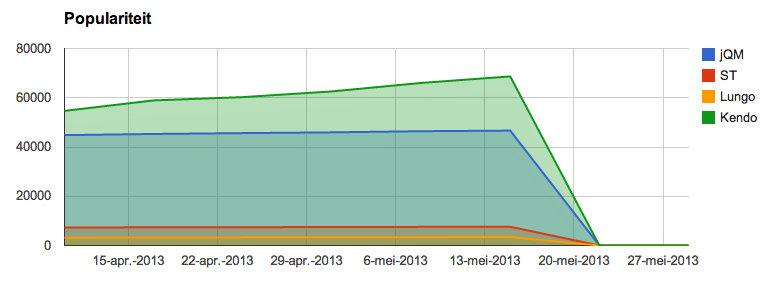
\includegraphics[width=\textwidth]{figuren/populariteit.png}
  \caption{Populariteit waargenomen over de periode van 15 april tot 22 mei 2013.}
  \label{fig:populariteit-evolutie}
\end{figure}

Als laatste wordt de populariteit aan de hand van Google Trends bekeken op figuur~\ref{fig:google-trends}.
Duidelijk is dat hier \jqm{} de grote winnaar is.
Sinds 2011 maakt het raamwerk een grote opmars door het uitbrengen van de eerste stabiele versie~1.0.
Eind 2012 kende \jqm{} echter een serieuze daling, maar deze werd terug een stijging omgezet door het uitbrengen van versie~1.3. 
\st{} kende een piek in maart 2012 bij het uitbrengen van \st{}~2.0.
Sinds begin 2012 maakt \kendo{} een opmars en als de trend zich verder zet, zal het \st{} inhalen.
Dit komt overeen met de waargenomen opmars van \kendo{} op figuur~\ref{fig:populariteit-evolutie}.
\lungo{} is nauwelijks op de grafiek waarneembaar.

\begin{figure}[H]
  \centering
  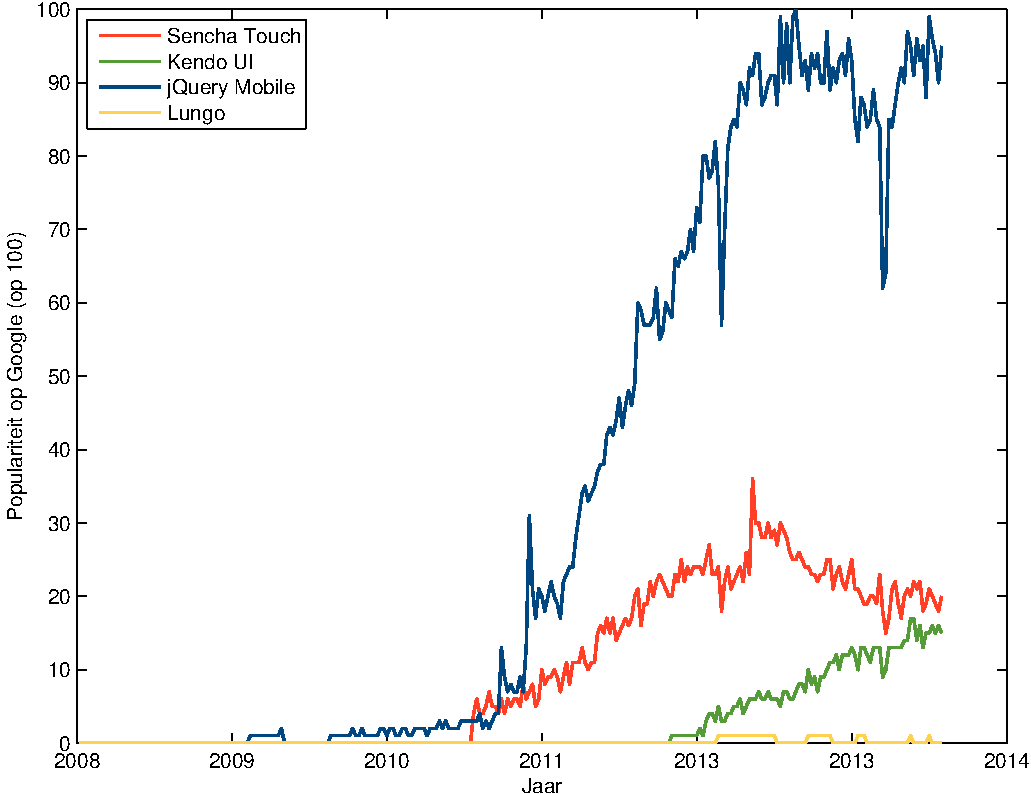
\includegraphics[width=\textwidth]{figuren/google-trends.pdf}
  \caption{Populariteit op Google Trends waargenomen van januari 2008 tot heden waarbij een resultaat van 100 overeenkomt met de grootste zoekinteresse~\cite{Google2012a}}
  \label{fig:google-trends}
\end{figure}
\section{Productiviteit}
\label{sec:evaluatie-productiviteit}

\begin{table}[H]
\centering
\pgfplotstabletypeset[
  col sep=comma,
  string type,
  header=true,
  columns={Productiviteit,jQM,ST,Kendo,Lungo},
  columns/Productiviteit/.style={column name=\textbf{Productiviteit}, column type={l}},  
  columns/jQM/.style={column name=\textbf{\jqm}, column type={c}},
  columns/ST/.style={column name=\textbf{\st}, column type={c}},
  columns/Kendo/.style={column name=\textbf{\kendo}, column type={c}},
  columns/Lungo/.style={column name=\textbf{\lungo}, column type={c}},
  every head row/.style={
    before row=\toprule,
    after row=\midrule},
  every last row/.style={
    after row=\bottomrule}
]{tabellen/productiviteit.csv}
\caption{Samenvattende tabel voor productiviteitscriterium}
\label{tabel:evaluatie-productiviteit}
\end{table}
\section{Gebruik}
\label{sec:evaluatie-gebruik}
Het gebruik van de vier raamwerken wordt samengevat in tabel \ref{tabel:evaluatie-gebruik}.
Het wordt opgedeeld per uitdaging en vervolgens zal het per sectie uitvoerig worden besproken per raamwerk.

\begin{table}[H]
\centering
\pgfplotstabletypeset[
  begin table=\begin{tabular}{p{8cm} p{1cm} p{1cm} p{1cm} p{1cm}},
  end table=\end{tabular},
  skip coltypes=true,
  col sep=comma,
  string type,
  header=true,
  columns={Uitdaging,jQM,ST,Kendo,Lungo},
  columns/Uitdaging/.style={column name=\textbf{Uitdaging}, column type={l}},  
  columns/jQM/.style={column name=\textbf{\jqma}, column type={c}},
  columns/ST/.style={column name=\textbf{\sta}, column type={c}},
  columns/Lungo/.style={column name=\textbf{\lungoa}, column type={c}},
  columns/Kendo/.style={column name=\textbf{\kendoa}, column type={c}},
  every head row/.style={
    before row=\toprule,
    after row=\midrule},
  every last row/.style={
  	before row=\midrule,
    after row=\bottomrule}
]{tabellen/gebruik.csv}
\caption{Samenvattende tabel voor gebruik}
\label{tabel:evaluatie-gebruik}
\end{table}

%%%%%%%%%%%%%

\subsection{U1: Formulieren}
In tabel \ref{tabel:evaluatie-gebruik-u1} worden de resultaten getoond van de vijf deeluitdaging van U1:~Formulieren.
Onder de tabel wordt per raamwerk verklaard waarom dat resultaat werd behaald.

\begin{table}[H]
\centering
\pgfplotstabletypeset[
  begin table=\begin{tabular}{p{8cm} p{1cm} p{1cm} p{1cm} p{1cm}},
  end table=\end{tabular},
  skip coltypes=true,
  col sep=comma,
  string type,
  header=true,
  skip coltypes=true,
  columns={Uitdaging,jQM,ST,Kendo,Lungo},
  columns/Uitdaging/.style={column name=\textbf{Uitdaging}, column type={l}},  
  columns/jQM/.style={column name=\textbf{\jqma}, column type={c}},
  columns/ST/.style={column name=\textbf{\sta}, column type={c}},
  columns/Lungo/.style={column name=\textbf{\lungoa}, column type={c}},
  columns/Kendo/.style={column name=\textbf{\kendoa}, column type={c}},
  every head row/.style={
    before row=\toprule,
    after row=\midrule},
  every last row/.style={
  	before row=\midrule,
    after row=\bottomrule}
]{tabellen/gebruik/u1.csv}
\caption{Gebruik voor U1: Formulieren}
\label{tabel:evaluatie-gebruik-u1}
\end{table}


\paragraph{\jqm} 
Voor het toevoegen van \term{placeholders} in de formuliervelden kon beroep worden gedaan op het \code{placeholder}-attribuut in HTML5. 
Labels zijn verplicht in \jqm{}, maar kunnen onzichtbaar worden gemaakt met de CSS-klasse \code{ui-hide-label}~\cite{JQuery2013}. 
Wat wel opmerkelijk is wanneer men een formulier invult, daarna verstuurt en dan terugkeert, het formulier nog alle waarden bevat. 
Men moet na het formulier te hebben verstuurd, zelf het formulier altijd leegmaken. 
Dit kan met behulp van \js{} via de \code{reset()}-functie op het formulier.
 
Voor de types van de formuliervelden werd beroep gedaan op de volgende types: \code{text}, \code{number} en \code{email}. 
%Deze zorgen ervoor dat op de mobiele apparaten aangepaste toetsenborden te voorschijn komen. 
Het \code{date} type werd echter niet gebruikt om wille van twee redenen.
Ten eerste was hiervoor een slechte ondersteuning naar mobiele browsers toe~\cite{Deveria2013b}.
Android~2.3 ondersteunt dit niet en de \term{placeholder}-tekst in het veld ontbrak op iOS~6 en Android~4.2.
Hierdoor weet de gebruiker in eerste instantie niet wat hij hier moet invullen. 
Zelf een \term{placeholder} instellen is onmogelijk voor een \code{date}-type~\cite{Berjon2012}. 
Een tweede probleem was het opleggen van het bereik van datums, wat met het \code{date}-type onmogelijk is. 
Beide problemen werden opgelost door gebruik te maken van de Date \& Time Picker van Mobiscroll~\cite{Mobiscroll2013} die ook aangepaste lay-out heeft conform met die van \jqm{}. 
Het veld heeft dan wel het type \code{text}.
Het is dus in principe mogelijk om iets anders dan een datum in te geven. 
Dit wordt belet door ook nog eens een datumvalidatie (zie \ref{sec:evaluatie-gebruik-u3}) te doen op dit tekstveld mocht de plug-in het niet hebben afgedwongen.
 
Het was ook nodig om enkel de maand en jaar in te geven als datum, dus zonder dag.
Ook hier kon niet het \code{date}-type gebruikt worden, omdat daar ook een dag voor nodig is. 
Daardoor werden de maanden handmatig geprogrammeerd als vaste lijstitems. 
De jaren zijn dynamisch en zijn telkens dit jaar, het volgende en het vorige jaar. 
Deze functionaliteit kon ook met de plug-in van Mobiscroll worden verwezenlijkt.

\paragraph{\st} 
% Placeholders, text, email and number fields are supported by the framework and can be easily created.  
% Labels can be avoided by not defining them.  
% Creating custom datepickers is not supported.  
% It is impossible to ignore the days field and only years can be delimited.  
% Clearing the form after it was send, has to be programmed manually.
Een formulier wordt in \st{} \code{fielset} genoemd.
Een \code{view} van een formulier voorzien kan door in de rij van elementen een object met \code{xtype} \code{fieldset} te maken.
Dit object kan op zijn beurt voorzien worden van een rij van elementen.
Volgende velden worden aangeboden in \st{}:
\begin{itemize}
  \item \code{textfield}        Ext.field.Text
  \item \code{numberfield}      Ext.field.Number
  \item \code{emailfield}	 Ext.field.Email			
  \item \code{textareafield}    Ext.field.TextArea
  \item \code{hiddenfield}      Ext.field.Hidden
  \item \code{radiofield}       Ext.field.Radio
  \item \code{checkboxfield}    Ext.field.Checkbox
  \item \code{selectfield}      Ext.field.Select	
  \item \code{togglefield}      Ext.field.Toggle
  \item \code{fieldset}         Ext.form.FieldSet
\end{itemize}

Tekst-, email en nummervelden worden bij het renderen tot HTML5-invoertypes omgevormd en bijgevolg worden op mobiele toestellen bijhorende virtuele toetsenborden weergegeven.
Een placeholder toevoegen kan door een veld met \code{placeholder} eigenschap te voorzien en de waarde aan de gewenste placeholder gelijk te stellen. 
Een label toevoegen verloopt analoog,  deze weglaten zal geen label renderen.

Een aangepaste \term{datepicker} maken is niet standaard voorzien.
Een standaard \term{datepicker} is echter wel voorzien met \code{datepicker} als xtype.
Deze kan enkel geconfigureerd worden door een begin- en eindjaar in te stellen.
Een \term{datepicker} maken waarbij het bereik kleiner is dan een jaar, is niet mogelijk.
Ook is het onmogelijk om enkel een maand- en jaarveld te tonen.

%TODO challenge bekijken (enkel reset oproepen normaal ok )
Het leegmaken van een formulier gebeurt niet automatisch wanneer het verzonden wordt.
Hiervoor moet de \code{reset} methode op het bijhorende \code{formpanel} worden opgeroepen.

\paragraph{\kendo}
 Formulierelementen definiëren kan via data-attributen door gebruik te maken van de opmaakgedreven aanpak van \kendo.
 Deze methodologie volgt dus sterk de HTML5-standaard.
 Het placeholder attribuut kan een placeholder definiëren,  het vermijden van een label zal geen labels genereren.
 Het type van het formulierelement moet met het type attribuut worden weergegeven.
 Volgende types worden door \kendo{} ondersteund:
 \begin{itemize}
  \item \code{text}
  \item \code{password}
  \item \code{search}
  \item \code{url}
  \item \code{email}
  \item \code{number}
  \item \code{tel}
  \item \code{file} (niet in iOS)
  \item \code{date}
  \item \code{timemonth} 
  \item \code{datetime}
 \end{itemize}

 \term{Datepickers} worden als widget aangeboden in het Web luik van \kendo{}.
 Het raamwerk zal een invoerelement omvormen naar een \code{kendoDatePicker}.
 Het invoerelement ziet er als volgt uit: \code{<input id=\"datepicker\"\/>}.  
 Vervolgens moet het element worden geïnitialiseerd met \code{\$("\#datePicker").kendoDatePicker()}.
 De datepicker is aanpasbaar zoals gevraagd in de POC.
 Het bereik van de data selectie kan worden ingeperkt door de \code{min} en \code{max} eigenschap van de \code{kendoDatePicker} te zetten.
 Deze eigenschappen worden bij initialisatie van het object meegegeven.
 Enkel maand- en jaarvelden tonen kan door de diepte van de \term{datepicker} in te stellen.
 Hiervoor moet de eigenschap \code{depth} aan \code{year} worden gelijkgesteld.
 
 Het wissen van formulieren steunt op de MVVM-architectuur.
 Een fomulier is gebonden aan een \code{(view)model}:  de inhoud van elk formulierelement komt overeen met de waarde van een eigenschap van een \code{(view)model} met dezelfde naam.
 Wanneer een uitgave wordt verzonden, zal de huidige waarde van het \code{(view)model} in een \js-object worden opgeslagen en wordt het \code{(view)model} gereset.
 Door de dubbele binding tussen formulier en \code{(view)model} zal ook de inhoud van de formulierelementen worden gewist.
 
 
\paragraph{\lungo} 
Het toevoegen van \term{placeholders} in de formuliervelden gebeurt met het HTML5-atttribuut \code{placeholder}.
In \lungo{} zijn labels niet verplicht.
Indien deze niet gewenst zijn, kunnen deze gewoon uit de HMTL5-code weggelaten worden.

De types \code{text}, \code{number} en \code{email} voor formuliervelden worden verwezenlijkt door deze als type voor de \code{input}-tags mee te geven in het formulier.
Gelijkaardig met de twee aangehaalde problemen voor \jqm{}, werd niet gekozen voor het \code{date}-type, maar een plug-in om de functionaliteit met datums op te lossen.
De \code{date-picker} werd gebruikt van de plug-in pagina van Lungo zelf~\cite{TapQuo2013b}.
Bij deze plug-in is al voorbeeldcode aanwezig die nodig is om automatisch een \term{datepicker} te openen en de aangeklikte datum in het formulierveld te zetten.
De plug-in laat echter niet toe om een bereik op te geven.
De datum met enkel een maand en jaar diende handmatig geprogrammeerd te worden omdat de aangeboden plug-in hiervoor geen ondersteuning bood.

Het legen van een formulier gebeurt in Lungo door de \code{reset}-functie in \js{} op te roepen op dat formulier.

%%%%%%%%%%%%%

\subsection{U2: Invullen van formulier}
In tabel \ref{tabel:evaluatie-gebruik-u2} worden de resultaten getoond van de twee deeluitdaging van U2:~Invullen van formulier.
Onder de tabel wordt per raamwerk verklaard waarom dat resultaat werd behaald.

\begin{table}[H]
\centering
\pgfplotstabletypeset[
  begin table=\begin{tabular}{p{8cm} p{1cm} p{1cm} p{1cm} p{1cm}},
  end table=\end{tabular},
  skip coltypes=true,
  col sep=comma,
  string type,
  header=true,
  columns={Uitdaging,jQM,ST,Kendo,Lungo},
  columns/Uitdaging/.style={column name=\textbf{Uitdaging}, column type={l}},  
  columns/jQM/.style={column name=\textbf{\jqma}, column type={c}},
  columns/ST/.style={column name=\textbf{\sta}, column type={c}},
  columns/Lungo/.style={column name=\textbf{\lungoa}, column type={c}},
  columns/Kendo/.style={column name=\textbf{\kendoa}, column type={c}},
  every head row/.style={
    before row=\toprule,
    after row=\midrule},
  every last row/.style={
  	before row=\midrule,
    after row=\bottomrule}
]{tabellen/gebruik/u2.csv}
\caption{Gebruik voor U2: Invullen van formulier}
\label{tabel:evaluatie-gebruik-u2}
\end{table}

\paragraph{\jqm}
Om een formulierveld in te vullen met data, dient eerst het formulierveld gezocht te worden en daarna zijn waarde gezet te worden.
Dit gebeurt typisch voor velden van het type \code{input} en \code{textarea} volgens de volgende code: \code{\$("form-veld").val("waarde")}.
Bij het \code{select}-type voor een veld kan deze code niet worden gebruik.
Hier moet de waarde worden gezocht in de lijst en dan aan de gevonden waarde het \code{selected}-attribuut worden toegevoegd.
Een gelijkaardige manier dient gevolgd te worden voor het \code{radio}-type voor een veld.
Ook hier moet eerst de waarde worden gezocht, waarna aan de gevonden waarde het \code{checked}-attribuut wordt toegevoegd.
Het vullen van formuliervelden wordt niet door \jqm{} geautomatiseerd, wat betekent dat dit dus voor iedere formulierveld dient te gebeuren.

Het \term{read-only} maken van velden gebeurt via het HTML-attribuut \code{readonly}.
Dit geld voor alle types van velden, behalve voor \code{radio}-elementen en \code{select}-items waar \code{disabled} wordt gebruikt.
Voor \code{select}-items moeten de andere niet-benodigde lijstitems verwijderd worden, want deze kunnen nog steeds aangeklikt worden.

\paragraph{\st}
Het invullen van een formulier wordt ondersteund door de MVC-architectuur.
Twee verschillende methoden worden in de POC gebruikt.
Een eerste maakt gebruik van de \code{setRecord} methode van een \code{formpanel}.
De modelinstantie die het formulier zal invullen als parameter worden meegeven.
\st{} zal automatisch de velden invullen waarbij de naam gelijk is aan de eigenschap van het model.
Zo kan tekst op tekstvelden worden gemapt,  nummers op numerieke velden en \code{booleans} op \code{togglefields}.
Een opmerking over het invullen van een \code{radiofield} moet worden gemaakt.
Een model kan worden voorzien met eigenschappen met volgende types:
\begin{itemize}
  \item auto (Default, implies no conversion)
  \item string
  \item int
  \item float
  \item boolean
  \item date
\end{itemize}
Er bestaat dus geen vlekkeloze mapping tussen een eigenschap van een model en een \code{radiofield}.
Hetzelfde geldt voor een \code{checkboxfield}.
Om deze in te vullen moet de \code{setGroupValue} van het veld worden aangesproken.


%TODO u13 lijsten en click invullen van formulier,  hier ook...
De tweede methode voor het invullen van formulieren maakt gebruikt van een \code{navigationview} en wordt in U13: Lijsten besproken.

Velden read-only maken kan door objecten te voozien van de \code{readOnly} eigenschap en de waarde op \code{true} te zetten.
Bij \code{radiofields} en \code{checkboxfields} heet deze eigenschap \code{disabled}.


\paragraph{\kendo}
Het invullen van een formulier steunt ook op de MVVM-architectuur en is gelijkaardig aan het resetten van een formulier.
De dubbele binding tussen een formulier en \code{(view)model} wordt met de HTML-tag \code{data-model} aangegeven.
Een \code{viewmodel} wordt in \kendo{} \code{ObservableObject} genoemd.
Een \code{model} heet \code{Model} en erft over van een \code{ObservableObject}.
Deze laatste breidt een \code{ObservableObject} uit met de mogelijkheid om schema's,  velden en methoden te definiëren.  
In wat volgt zal aangenomen worden dat een \code{ObservableObject} wordt gebruikt in plaats van een \code{Model},  tenzij anders vermeld.
Om een formulier met data te vullen is het de taak van de programmeur de velden van het \code{ObservableObject} van de correct waarden te voorzien.
De gebonden formulierelementen zullen vervolgens automatisch worden ingevuld.


Read-only velden moeten in het data-attribuut van het formulierelement worden gespecificeerd.
Alle invoer types buiten radio- en selectknoppen gebruiken hiervoor het \code{readOnly} sleutelwoord.
Radio- en selectknoppen worden onbeschikbaar met het \code{disabled} sleutelwoord.

\paragraph{\lungo}
Velden vullen met data dient handmatig te gebeuren door eerst het formulierveld op te zoeken en daarna de waarde te zetten.
Dit gebeurt typisch volgens de volgende code: \code{\$\$("\#form-veld").val("waarde")}.
Deze functie kan ook gebruikt worden voor \code{select}-types.
Geoptimaliseerde mobiele lay-out voor \code{radio}-types is niet aanwezig in \lungo.
Een opmerking dient wel gemaakt te worden dat de waarde altijd een \code{string} moet zijn.
Dit betekent dus voor getallen dat deze altijd eerst moeten worden omgevormd met de \js{}-functie \code{toString()}. 

Het \term{read-only} maken van velden gebeurt via het HTML-attribuut \code{readonly}.
Dit gaat voor alle types van velden, behalve voor \code{select}-types.
Daar worden de niet-benodigde lijstitems verwijderd en wordt de \code{select} zelf \code{disabled} gemaakt.

%%%%%%%%%%%%%

\subsection{U3: Formuliervalidatie}
\label{sec:evaluatie-gebruik-u3}

In tabel \ref{tabel:evaluatie-gebruik-u3} worden de resultaten getoond van de vier deeluitdaging van U3: Formuliervalidatie.
Onder de tabel wordt per raamwerk verklaard waarom dat resultaat werd behaald.


\begin{table}[H]
\centering
\pgfplotstabletypeset[
  begin table=\begin{tabular}{p{8cm} p{1cm} p{1cm} p{1cm} p{1cm}},
  end table=\end{tabular},
  skip coltypes=true,
  col sep=comma,
  ignore chars={\"},
  verb string type,
  header=true,
  columns={Uitdaging,jQM,ST,Kendo,Lungo},
  columns/Uitdaging/.style={column name=\textbf{Uitdaging}, column type={l}},  
  columns/jQM/.style={column name=\textbf{\jqma}, column type={c}},
  columns/ST/.style={column name=\textbf{\sta}, column type={c}},
  columns/Lungo/.style={column name=\textbf{\lungoa}, column type={c}},
  columns/Kendo/.style={column name=\textbf{\kendoa}, column type={c}},
  every head row/.style={
    before row=\toprule,
    after row=\midrule},
  every last row/.style={
  	before row=\midrule,
    after row=\bottomrule}
]{tabellen/gebruik/u3.csv}
\caption{Gebruik voor U3: Formuliervalidatie}
\label{tabel:evaluatie-gebruik-u3}
\end{table}

\paragraph{\jqm}
Validatie is niet standaard aanwezig in jQuery Mobile. 
Eerst werd geprobeerd om de verplichte velden te voorzien van het \code{required}-attribuut in HTML5. 
Dit werd niet gedaan om twee redenen.
Enerzijds is hiervoor geen ondersteuning voor mobiele browsers~\cite{Deveria2013}. 
Anderzijds is het ook nodig om de velden te valideren op hun waarde.
Als oplossing werd de plug-in van Jörn Zaefferer gebruikt~\cite{Zaefferer2013}. 
Deze lost beide problemen op.
De plug-in zelf kan op twee manieren gebruikt worden: enerzijds annoteren van de formuliervelden met speciale CSS-klassen in de HTML-code ofwel anderzijds door programmatie met \js{}. 
Beide aanpakken werden getest en slaagden. 

De plug-in bevat de volgende ingebakken validatieregels die nodig waren: \code{required}, \code{number}, \code{email} en \code{date}.
Daarnaast was het nodig dat een veld verplicht was enkel indien een bepaalde optie aangevinkt was.
Zo een afhankelijkheidsrelatie is standaard aanwezig in de plug-in.

De plug-in toont standaard een foutboodschap onder het foute formulierveld.
Door de uitgebreide API van de plug-in die ook uitvoerig gedocumenteerd is, konden alle foutboodschappen samen in een dialoogvenster worden weergegeven.

Een specifiek mobiel probleem was dat bij het tonen van het dialoogvenster, de plug-in op de achtergrond de cursor op het eerste veld zette. 
Hierdoor verscheen het toetsenbord op het scherm van het mobiele apparaat wanneer het dialoogvenster tevoorschijn kwam, wat niet de bedoeling is. 
Dit werd opgelost door \code{focusInvalid:false} in te stellen in de plug-in.

De plug-in annoteert de foute velden met de CSS-klasse \code{error}.
Hierdoor kon de rode rond in CSS worden geprogrammeerd. 
Dit ging voor \code{input} en \code{textarea}, maar gaf problemen voor \code{select} en \code{fieldset}.
Door de extra code die \jqm{} genereert rond deze velden, moest via de DOM de omringende code geannoteerd worden om de rode rand te bekomen. 
Deze functie kon aangehaakt worden op de \code{highlight} en \code{unhighlight} functies van de plug-in.

\paragraph{\st}
Een model kan worden voorzien van validatieregels.
Deze regels worden als objecten in een rij aan de \code{validations} eigenschap van een model toegekend.
Volgende validatieregels zijn ingebouwd:
\begin{description}
  \item [presence] verzekert dat het het veld een waarde heeft waarbij nul als geldig wordt beschouwd,  lege tekst niet.
  \item [length] verzekert dat een text een minimale en/of maximale waarde heeft.
  \item [format] verzekert dat een text voldoet aan een opgegeven reguliere expressie.
  \item [inclusion] verzekert dat de waarde van een veld gelijk is aan een element van een gespecifieerde set.
  \item [exclusion] verzekert dat de waarde van een veld zeker niet gelijk is aan een element van een gespecifieerde set.
\end{description}
De controle of een opgegeven waarde een nummer is kan met de \code{format} regel en de \code{/\d+/} reguliere expressie.
Om een bepaalde modelinstantie te valideren moet de \code{validate} methode op de instantie worden opgeroepen.
Om eigen validatieregels toe te laten moet de implementatie van deze methode worden overschreven. \footnote{Informatie gevonden op \exturl{www.sencha.com/forum/showthread.php?122680-Conditional-fields-validations}}
Deze functionaliteit zit dus niet standaard in \st{}.
Met de nieuwe \code{validate} methode kan een \code{validator} aan een validatieregel worden toegevoegd.
Dit is een functie die de programmeur zelf bepaalt en \code{true} of \code{false} teruggeeft bij het al dan niet slagen van een conditie.

Het opbouwen van een foutenboodschap kan door te itereren over de fouten die na validtie werden teruggevonden.
Een specifieke foutenboodschap kan aan elke validatieregel worden toegekend.

Invalide formulierelementen aanduiden met een rode rand wordt niet door \st{} ondersteund.
Hiervoor moet CSS worden gebruikt.
Foutief ingevulde formulierelementen moeten na valiatie met een CSS-klasse worden aangevuld.

\paragraph{\kendo}
Het \kendo{} raamwerk ondersteunt de validaties zoals aangeboden binnen HTML5:
\begin{itemize}
  \item [required] verzekert dat een het veld een waarde heeft.
  \item [pattern] verzekert dat de waarde van een veld voldoet aan een opgegeven reguliere expressie.
  \item [min/max] verzekert dat de waarde van een veld groter en/of kleiner is dan een opgegeven waarde.
  \item [data types] verzekert dat de waarde van een veld gelijk is aan het opgegeven type (e-mail, url, number, enz.)
\end{itemize}
Deze validaties moeten binnen het data-attribuut van het formulierelement worden aangebracht.

De \kendo{} \code{validator} is compatibel met deze HTML5-validaties.
Een \code{validator} moet in \js worden aangemaakt met volgend commando:  \code{\$("\#myform").kendoValidator().data("kendoValidator")}.
Hierbij kan de jQuery selector eender welk element uit het DOM aanduiden.
De \code{validator} zal geselecteerde invoerelementen controleren op validatieregels.

Eigen condities kunnen als validatieregels worden geformuleerd als \js-functie die \code{true} teruggeeft als de validatie slaagt.
Deze functie kan aan de set van regels van een \code{validator} worden toegevoegd.
De validatiecontrole starten kan door de \code{validate} methode op de \code{validator} op te roepen.
Bij het controleren van invoerelementen worden altijd eerst de standaard validatieregels gecontoleerd,  daarna de eigen validatieregels.
De volgorde waarin de controles worden uitgevoerd ligt vast en zal stoppen zodra één controle mislukt.

%TODO mijn tricky implementatie van other -> remkars validatie vermelden?

Validatieberichten kunnen voor standaard validaties door het raamwerk zelf worden opgebouwd.
Deze kunnen worden overschreven door zelf een data-attribuut \code{validationMessage} aan het invoerelement toe te kennen.
Bij eigen validatieregels kan een validatiebericht per regel worden gespecificeerd.

Invalide formulierelementen aanduiden met een rode rand wordt niet door \kendo{} ondersteund.
De standaard implementatie voorziet een \code{tooltip} per invalied veld.
Deze zal het validatiebericht naast het invalide formulierelement plaatsen. 

Een venster tonen waarbij alle foutenboodschappen zijn samengevat is ook niet standaard aanwezig.
De \code{errors} methode van een \code{validator} geeft een rij van foutenboodschappen terug.
De volledige foutenboodschap moet vervolgens worden geconstrueerd door alle foutenboodschappen te concateneren.
Hoe een dialoogvenster gemaakt wordt zal in U11.2 Toon dialoog worden besproken.

\paragraph{\lungo}
%TODO Tim: moet ik ook uitleggen hoe ik het geprogrammeerd heb? score is toch 0..
Validatie is niet aanwezig in Lungo en er kon ook geen plug-in voor QuoJS gevonden worden~\cite{Ameye2013}.
Er werd geprobeerd om bestaande plug-ins voor andere \js{}-bibliotheken om te vormen en deze te laten werken met QuoJS.
Aangezien deze manier niet direct een oplossing bracht, werd alle validatie manueel geprogrammeerd.
%TODO Tim: Voor de quotering blijft het resultaat hetzelfde.
Door de slechte mobiele ondersteuning werd er ook geen beroep gedaan op HTML5-valdiatie.
Het tonen van foutboodschappen alsook het tonen van een rode rand rond de foute velden werd ook zelf geprogrammeerd.

%%%%%%%%%%%%%

\subsection{U4: Handtekening}
In tabel \ref{tabel:evaluatie-gebruik-u4} worden de resultaten getoond van de deeluitdaging van U4: Handtekening.
Onder de tabel wordt per raamwerk verklaard waarom dat resultaat werd behaald.

\begin{table}[H]
\centering
\pgfplotstabletypeset[
  begin table=\begin{tabular}{p{8cm} p{1cm} p{1cm} p{1cm} p{1cm}},
  end table=\end{tabular},
  skip coltypes=true,
  col sep=comma,
  string type,
  header=true,
  columns={Uitdaging,jQM,ST,Kendo,Lungo},
  columns/Uitdaging/.style={column name=\textbf{Uitdaging}, column type={l}},  
  columns/jQM/.style={column name=\textbf{\jqma}, column type={c}},
  columns/ST/.style={column name=\textbf{\sta}, column type={c}},
  columns/Lungo/.style={column name=\textbf{\lungoa}, column type={c}},
  columns/Kendo/.style={column name=\textbf{\kendoa}, column type={c}},
  every head row/.style={
    before row=\toprule,
    after row=\midrule},
  every last row/.style={
  	before row=\midrule,
    after row=\bottomrule}
]{tabellen/gebruik/u4.csv}
\caption{Gebruik voor U4: Handtekening}
\label{tabel:evaluatie-gebruik-u4}
\end{table}

\paragraph{\jqm}
Er werd gezocht naar een plug-in om deze functionaliteit te bekomen, doordat \jqm{} dit niet standaard aanbiedt. 
Eerst werd gewerkt met Signature Pad van Thomas Bradley~\cite{Bradley2013}. 
Door de lange tijd die werd besteed aan het aanpassen van de lay-out, werd overgestapt naar jSignature van Willow Systems~\cite{Systems2013}. 
Deze laatste gaf ook het voordeel dat de breedte van het gebied om te handtekening in te zetten, zich automatisch naar 100\% schaalde. 
De plug-in maakt gebruik van het HTML5 \code{canvas}-element en de \code{.toDataURL()} methode.
Hierdoor kan de base64-string bekomen worden die nodig is om door te sturen naar de server.
%TODO TIM: verplaatsen
%Deze wordt echter niet ondersteund op Android versies 2.3 en lager~\cite{Systems2013} waardoor de functionaliteit op die toestellen niet werkt.

\paragraph{\st}
Het tekenen van een handtekening steunt op een plug-in van SimFla~\cite{SimFla2011} en is in de Sencha Market te vinden op \exturl{market.sencha.com/extensions/signature-pad-field}.
Een plug-in aan het raamwerk toevoegen kan door het \js-bestand in de touch/src/ux folder te plaatsen.
Vervolgens moet de plug-in worden geladen bij het initialiseren van de applicatie.

De plug-in maakt een nieuw xtype \code{signaturefield} beschikbaar dat als veld in een formulier kan worden gebruikt.

De plug-in maakt gebruikt van het HTML5-canvas en retourneert de handtekening als geëncodeerde base64-tekst.

\paragraph{\kendo}
Aangezien \kendo{} steunt op de jQuery bibliotheek is \kendo{} ook perfect compatibel met jQuery plug-ins.
Net zoals bij \jqm{} werd ook de jSignature handtekening van Willow Systems~\cite{Systems2013} geïmplementeerd.

\paragraph{\lungo}
Het maken van een handtekening is niet standaard aanwezig en daarenboven kon ook geen plug-in  worden gevonden.
Er kan echter worden gebruik gemaakt van plug-ins die op andere \js{}-bibliotheken dan QuoJS steunen, maar de auteurs besloten om deze niet te beschouwen.
Daarenboven zouden er dan ook twee \js{}-bibliotheken aanwezig zijn in de applicatie.

%%%%%%%%%%%%%
\subsection{U5: Toon PDF}
In tabel \ref{tabel:evaluatie-gebruik-u5} worden de resultaten getoond van de twee deeluitdagingen van U5:~Toon PDF.
Onder de tabel wordt per raamwerk verklaard waarom dat resultaat werd behaald.

\begin{table}[H]
\centering
\pgfplotstabletypeset[
  begin table=\begin{tabular}{p{8cm} p{1cm} p{1cm} p{1cm} p{1cm}},
  end table=\end{tabular},
  skip coltypes=true,
  col sep=comma,
  string type,
  header=true,
  columns={Uitdaging,jQM,ST,Kendo,Lungo},
  columns/Uitdaging/.style={column name=\textbf{Uitdaging}, column type={l}},  
  columns/jQM/.style={column name=\textbf{\jqma}, column type={c}},
  columns/ST/.style={column name=\textbf{\sta}, column type={c}},
  columns/Lungo/.style={column name=\textbf{\lungoa}, column type={c}},
  columns/Kendo/.style={column name=\textbf{\kendoa}, column type={c}},
  every head row/.style={
    before row=\toprule,
    after row=\midrule},
  every last row/.style={
  	before row=\midrule,
    after row=\bottomrule}
]{tabellen/gebruik/u5.csv}
\caption{Gebruik voor U5: Toon PDF}
\label{tabel:evaluatie-gebruik-u5}
\end{table}

\paragraph{\jqm}
AJAX is bedoeld om tekst op te halen, maar geen ruwe data zoals een PDF~\cite{Scott2009}. 
Hierdoor werd gebruik gemaakt van een verborgen formulier met de nodige parameters die de PDF ophaalt bij de backend. 
Bij het klikken op een lijstitem in het overzicht, wordt dit verborgen formulier opgestuurd naar de \term{backend} die dan een PDF teruggeeft in de browser. 
Het weergeven van de PDF wordt overgelaten aan het mobiel apparaat dat de correcte applicatie hiervoor opstart.

\paragraph{\st}
Het tonen van een PDF steunt op een plug-in van Fiedler~\cite{Fiedler2012} en kan op de Sencha Market gevonden worden op \exturl{market.sencha.com/extensions/pdf-viewer-panel}.
Het tonen van een PDF-bestand kan door de huidige \code{view} te wijzigen naar een \code{Ext.ux.PDF view}.
Deze \code{view} bestaat uit een paneel met een hoofdtekst.
Het paneel toont één pagina van het PDF-bestand,  de hoofdtekst bevat de navigatie naar andere pagina's.

Om de plug-in in de POC in te passen waren echter twee aanpassingen noodzakelijk.
Het PDF-bestand moet via een POST verzoek worden opgehaald waarbij parameters het exacte PDF-bestand aanduiden.
Ook moest er een terugknop in de hoofdtekst van het paneel worden aangebracht om terug naar het overzicht van doorgestuurde formulieren te gaan.
Beide aanpassingen moesten in het \js-bestand van de plug-in worden aangebracht.

\paragraph{\kendo}
De implementatie voor het tonen van het PDF-bestand is analoog als de \jqm{} implementatie.
%TODO terug aanhalen? Aan elk lijstelement in het overzicht van uitgavenformulieren wordt een functie gebonden.

\paragraph{\lungo}
AJAX is bedoeld om tekst op te halen, maar geen ruwe data zoals een PDF~\cite{Scott2009}. 
Hierdoor werd gebruik gemaakt van een omweg door een verborgen formulier te versturen die de PDF ophaalt.
In dat verborgen formulier worden de nodige parameters ingevoerd en zal het op de achtergrond  worden verstuurd, net zoals een gebruiker dat zou doen.
Daarna wordt het PDF-bestand gestuurd naar de gebruiker.
Het weergeven van de PDF wordt overgelaten aan het mobiel apparaat dat de correcte applicatie hiervoor opstart.

%%%%%%%%%%%%%
\subsection{U6: Toevoegen van afbeelding}
In tabel \ref{tabel:evaluatie-gebruik-u6} worden de resultaten getoond van de drie deeluitdagingen van U6:~Toevoegen van afbeelding.
Onder de tabel wordt per raamwerk verklaard waarom dat resultaat werd behaald.

\begin{table}[H]
\centering
\pgfplotstabletypeset[
  begin table=\begin{tabular}{p{8cm} p{1cm} p{1cm} p{1cm} p{1cm}},
  end table=\end{tabular},
  skip coltypes=true,
  col sep=comma,
  string type,
  header=true,
  columns={Uitdaging,jQM,ST,Kendo,Lungo},
  columns/Uitdaging/.style={column name=\textbf{Uitdaging}, column type={l}},  
  columns/jQM/.style={column name=\textbf{\jqma}, column type={c}},
  columns/ST/.style={column name=\textbf{\sta}, column type={c}},
  columns/Lungo/.style={column name=\textbf{\lungoa}, column type={c}},
  columns/Kendo/.style={column name=\textbf{\kendoa}, column type={c}},
  every head row/.style={
    before row=\toprule,
    after row=\midrule},
  every last row/.style={
  	before row=\midrule,
    after row=\bottomrule}
]{tabellen/gebruik/u6.csv}
\caption{Gebruik voor U6: Toevoegen van afbeelding}
\label{tabel:evaluatie-gebruik-u6}
\end{table}

\paragraph{\jqm}
Het toevoegen van een afbeelding gebeurt door \code{file} als invoertype van het formulierveld te gebruiken. 
In versie~1.2 wordt dit veld nog niet opgemaakt met lay-out, maar dit gebeurt wel in versie 1.3~\cite{JQuery2013d}. 
Het omvormen van de afbeelding naar base64 werd geïmplementeerd met de FileReaderAPI en het canvas, wat beide HTML5-specificaties zijn. 
De aangeklikte afbeelding wordt gelezen door middel van de FileReaderAPI, waarna het tijdelijk als afbeelding wordt opgeslagen en daarna geïmporteerd wordt op het canvas. 
Eenmaal geïmporteerd, kan de functie \code{.toDataURL()} opgeroepen worden op het canvas om de geïmporteerde afbeelding om te vormen naar base64. 

Het voorvertonen van het geüploade afbeelding hangt af van het mobiele besturingssysteem.
Zo wordt op iOS~6 een miniatuurafbeelding getoond, terwijl op Android de bestandsnaam wordt getoond.
Het is natuurlijk ook mogelijk om de preview na conversie zelf te tonen op het scherm.
Bij iOS zouden er dan twee voorvertoningen te zien zijn op hetzelfde scherm.

%TODO Tim: verplaatsen naar ondersteuning
% Deze aanpak werkt correct op recente mobiele apparaten. 
% De FileReaderAPI wordt echter niet ondersteund op Android versies 2.3 en lager of iOS versies lager dan 6.0~\cite{Deveria2013a} waardoor het opladen van een bewijs niet werkt.

\paragraph{\st}
Het opladen van een afbeelding steunt op een plug-in van Smirnov~\cite{Smirnov2012} en kan in de Sencha Market gevonden worden op \exturl{market.sencha.com/extensions/file-uploading-component-for-sencha-touch}.
De plug-in is generiek voor het opladen van elk type bestand,  niet uitsluitend afbeeldingen.
Het \js-bestand moet in de touch/src/ux folder worden geplaatst en de \code{Ext.ux.Fileup} klasse moet worden geïnitialiseerd.
Het xtype \code{img} wordt dan beschikbaar voor \st{} componenten.

De plug-in voorziet twee modes voor het opladen van bestanden: lokale als base64 of extern naar een server.
De eerste laat toe afbeeldingen in het DOM of \term{local storage} te laden.
Dit laatste is een aspect van de POC.

Nadat een bestand is opgeladen kunnen twee gebeurtenissen zich voordoen:  \code{loadsuccess} of \code{loadfailure}.
Het is de taak van een \code{controller} om deze gebeurtenissen op te vangen en een bijhorende methode te definiëren.
De succes functie krijgt de base64 text mee en kan een voorbeeld van de afbeelding laten weergeven.

\paragraph{\kendo}
\kendo{} Web biedt een widget aan die het opladen van bestanden toelaat.
Deze widget kan in twee modes worden gebruikt: syncroon of asynchroon.
Een HTML-invoerelement met \code{id} moet worden toegevoegd en geïnitialiseerd met \code{\$("\#id").kendoUpload()}.
In synchrone wordt het formulier met het oplaadelement verzonden naar de \term{backend} als een uitgave wordt toegevoegd.
In asynchrone mode gebeurt het opladen meteen na het selecteren van de afbeelding.
Deze methode voor het opladen van bestanden steunt op de HTML5 File API.
Het verzoek naar de \term{backend} is een POST-verzoek met \code{Content Type} \code{multipart/form-data}.
Omdat een voorbeeld van afbeelding werd gevraagd, is de asynchrone oplossing gekozen.	
\kendo{} voorziet \term{backend} integratie met ASP.NET MVC,  JSP en PHP.
Voor deze drie technologieën is een implementatie beschikbaar om het opladen van bestanden aan serverzijde af te handelen.
Er werd gekozen om de PHP-implementatie te gebruiken.
Wanneer een afbeelding succesvol is opgeladen, wordt de \code{success callback} opgeroepen met het bestand als parameter.
Het bestand wordt met een \code{FileReader} gelezen,  aan een \code{canvas} toegevoegd en naar base64 omgezet met de \code{toDataURL} methode.
Deze werkwijze is aanloog aan de \jqm{} implementatie.



\paragraph{\lungo}
Een afbeelding kiezen gebeurt door het formulierveld met het type \code{file} toe te voegen.
Het omvormen van de afbeelding naar base64 werd geïmplementeerd met de FileReaderAPI en het canvas, wat beide HTML5-specificaties zijn. 
De aangeklikte afbeelding wordt gelezen door middel van de FileReaderAPI, waarna het tijdelijk als afbeelding wordt opgeslagen en daarna geïmporteerd wordt op het canvas. 
Eenmaal geïmporteerd, kan de functie \code{.toDataURL()} opgeroepen worden op het canvas om de geïmporteerde afbeelding om te vormen naar base64. 

Het voorvertonen van het geüploade afbeelding hangt af van het mobiele besturingssysteem.
Zo wordt op iOS~6 een miniatuurafbeelding getoond, terwijl op Android de bestandsnaam wordt getoond.
Het is natuurlijk ook mogelijk om de preview na conversie zelf te tonen op het scherm.
Bij iOS zouden er dan twee voorvertoningen te zien zijn op hetzelfde scherm.

%%%%%%%%%%%%%
\subsection{U7: Auto-aanvullen}
In tabel \ref{tabel:evaluatie-gebruik-u7} worden de resultaten getoond van de twee deeluitdagingen van U7:~Auto-aanvullen.
Onder de tabel wordt per raamwerk verklaard waarom dat resultaat werd behaald.

\begin{table}[H]
\centering
\pgfplotstabletypeset[
  begin table=\begin{tabular}{p{8cm} p{1cm} p{1cm} p{1cm} p{1cm}},
  end table=\end{tabular},
  skip coltypes=true,
  col sep=comma,
  string type,
  header=true,
  columns={Uitdaging,jQM,ST,Kendo,Lungo},
  columns/Uitdaging/.style={column name=\textbf{Uitdaging}, column type={l}},  
  columns/jQM/.style={column name=\textbf{\jqma}, column type={c}},
  columns/ST/.style={column name=\textbf{\sta}, column type={c}},
  columns/Lungo/.style={column name=\textbf{\lungoa}, column type={c}},
  columns/Kendo/.style={column name=\textbf{\kendoa}, column type={c}},
  every head row/.style={
    before row=\toprule,
    after row=\midrule},
  every last row/.style={
  	before row=\midrule,
    after row=\bottomrule}
]{tabellen/gebruik/u7.csv}
\caption{Gebruik voor U7: Auto-aanvullen}
\label{tabel:evaluatie-gebruik-u7}
\end{table}

\paragraph{\jqm}
Indien er wordt gebruik gemaakt van versie~1.2 is een plug-in nodig om auto-aanvulling te bekomen.
Hiervoor kan de plug-in van Andy Matthews worden gebruikt~\cite{Matthews2013}. 
Dit is een zeer gemakkelijk te integreren plug-in die zowel met lokale data als data op afstand kan werken.
Sinds versie~1.3 voorziet \jqm{} deze functionaliteit zelf~\cite{JQuery2013c}.
Er wordt aangehaakt op het \code{listviewbeforefilter}-\term{event} waarbij een eigen filterfunctie geschreven kan worden.
De voorbeeldcode op de site kon integraal worden gebruikt. 

\paragraph{\st}
Het automatisch aanvullen van een formulierelement steunt op een plug-in van Tajur~\cite{Tajur2012}.
Deze plug-in is niet op de Sencha Market terug te vinden.
Door het \js-bestand toe te voegen wordt het xtype \code{autocompletefield} beschikbaar.
Een object met dit xtype kan een \code{proxy} definiëren die de server kan aanspreken om suggesties asynchroon op te halen.
Ook is het mogelijk het maximaal aantal suggesties vast te leggen.

De \term{backend} server die bij de POC hoort geeft bij een bepaald sleutelwoord suggesties in een JSON-rij terug.
De rij is voorzien van een sleutel maar alle elementen van de rij hebben geen sleutel.
\st{} voorziet vier methoden om de resultaten van een \code{proxy} te parsen naar modelinstanties:
\begin{description}
 \item [\code{JsonReader}] parst JSON-sleutels naar model velden.
 \item [\code{XmlReader}] parst XML-tags naar model velden.
 \item [\code{ArrayReader}] mapt elementen van een rij op velden van een model.
\end{description}
Geen van voorgaande methoden was in staat de rij met suggesties te parsen van rij-element naar modelinstantie.
Hierdoor kon geen klikbare dropdownmenu worden getoond.

\paragraph{\kendo}
Het automatisch aanvullen van een formulierelement wordt als widget door \kendo{} Web aangeboden.
Een HTML-invoerelement met id met worden aangemaakt en geinitialiseerd met \code{\$("\#id").kendoAutoComplete()}.
Elementen die automatisch aanvullen kunnen zowel van een lokale als externe bron worden aangeleverd.
Externe suggesties moeten via een \code{dataSource} worden ingeladen.
Een \code{DataSource} ondersteunt alle CRUD (\term{Create, Read, Update en Delete}) operaties en het sorteren, pagineren, filteren, groeperen en aggregeren van data.
Deze moet geconfigureerd worden om suggesties van de \term{backend} op te halen.
Buiten een \code{DataSource} kan het minimale aantal suggesties en een filter worden opgegeven.
De filter bepaalt de methode om suggesties op te halen:  en kan \code{startswith}, \code{endswith} of \code{contains} zijn.

\paragraph{\lungo}
Standaard biedt \lungo{} geen auto-aanvullig aan, maar wel op zijn site van plug-ins~\cite{TapQuo2013b}.
Daar werd de plug-in AutoComplete gebruikt.
De voorbeeldcode maakt het gemakkelijk om onmiddellijk een werkend voorbeeld van de plug-in te hebben.
Veel code kon dus gewoon worden overgenomen.

%%%%%%%%%%%%%
\subsection{U8: AJAX}
In tabel \ref{tabel:evaluatie-gebruik-u8} worden de resultaten getoond van de vier deeluitdagingen van U8:~AJAX.
Onder de tabel wordt per raamwerk verklaard waarom dat resultaat werd behaald.

\begin{table}[H]
\centering
\pgfplotstabletypeset[
  begin table=\begin{tabular}{p{8cm} p{1cm} p{1cm} p{1cm} p{1cm}},
  end table=\end{tabular},
  skip coltypes=true,
  col sep=comma,
  string type,
  header=true,
  columns={Uitdaging,jQM,ST,Kendo,Lungo},
  columns/Uitdaging/.style={column name=\textbf{Uitdaging}, column type={l}},  
  columns/jQM/.style={column name=\textbf{\jqma}, column type={c}},
  columns/ST/.style={column name=\textbf{\sta}, column type={c}},
  columns/Lungo/.style={column name=\textbf{\lungoa}, column type={c}},
  columns/Kendo/.style={column name=\textbf{\kendoa}, column type={c}},
  every head row/.style={
    before row=\toprule,
    after row=\midrule},
  every last row/.style={
  	before row=\midrule,
    after row=\bottomrule}
]{tabellen/gebruik/u8.csv}
\caption{Gebruik voor U8: AJAX}
\label{tabel:evaluatie-gebruik-u8}
\end{table}


\paragraph{\jqm}
Het maken van oproepen via AJAX gebeurt door jQuery. 
Dit gebeurt met de functie \code{\$.ajax} waar onder andere kan ingesteld worden wat het te verwachten antwoord is (zoals tekst, JSON of XML). 
Bij het succesvol uitvoeren van de oproep wordt de \code{succes}-functie opgeroepen, bij faling de \code{error}-functie waarna een relevante foutboodschap wordt getoond.

In jQuery is de functie \code{parseJSON} aanwezig, maar aangezien in de AJAX-oproep ingesteld wordt dat JSON wordt verwacht, parst jQuery al automatisch het antwoord. 
Hierdoor is de functie \code{parseJSON} niet nodig en kunnen direct worden omgaan met het antwoord.

Net zoals bij JSON het geval was, is het ook niet nodig om expliciet de \code{parseXML}-functie te gebruiken. 
Het doorlopen en opvragen van gegevens uit het XML-bestand vraagt meer werk. 
Waar er bij JSON direct kon worden omgegaan met de data, moet bij XML dat gebeuren aan de hand van selectoren.

Het versturen van JSON is gelijkaardig met het versturen van andere data.
Eerst zal de JSON-data moeten worden omgezet naar een string, wat gebeurt door \code{JSON.stringify}.
Daarna zal in de AJAX-oproep moeten worden aangegeven  dat de inhoud JSON is.
Dit gebeurt door \code{contentType: "application/json"} te schrijven.

\paragraph{\st}
AJAX-verzoeken kunnen zowel expliciet via een directe oproep met \code{Ext.Ajax.request} als impliciet via \code{stores} worden uitgevoerd.
De expliciete oproep is gelijkaardig aan de \code{\$.ajax} methode van jQuery.
Een enige uitzondering is te vinden bij kruis-domein AJAX-verzoeken.
Om aan de CORS-standaarden (Cross-Origin Resource Sharing) te voldoen moet de eigenschap \code{useDefaultXhrHeader} op \code{false} worden gezet.
%TODO referentie cors + opzoeken options request

De tweede,  impliciete,  methode voor AJAX-verzoeken is via \code{stores}.
Een \code{store} wordt voorzien van een \code{proxy}.  
Deze kan data aan de klant of server zijde opslaan.  
Een \code{proxy} voor opslag aan client zijde kan zowel in het RAM-geheugen als in de \term{local storage} en \term{session storage} van de browser opslaan.  
Een \code{proxy} voor server opslag kan data verzenden via AJAX (zelfde domein) of JSONP (verschillende domeinen).  
Een \code{proxy} kan ook geconfigureerd worden met \code{readers} en \code{writers} om data van de server te lezen of naar de server te schrijven.

Het verzenden van een JSON-\term{payload} moet via een expliciet AJAX-verzoek gebeuren.
Data kan via \code{Ext.encode} naar JSON worden geëncodeerd en via de \code{jsonData} eigenschap aan het verzoek worden gekoppeld.

\paragraph{\kendo}
Om asynchrone verzoeken naar de \term{backend} te implementeren, moet een \code{DataSource} worden gebruikt.
Zoals reeds besproken in de vorige uitdaging biedt dit object CRUD operaties.
Dit kan zowel op lokale (\js-objecten en \js-rijden) als externe data (XML, JSON, JSONP).
De \code{transport} eigenschap kan de configuraties bevatten om data te creëren (\code{create} eigenschap),  lezen (\code{read} eigenschap),  verwijderen (\code{destroy} eigenschap) en op te waarderen (\code{update} eigenschap).
Deze vier eigenschappen moeten geconfigureerd worden zoals de \code{\$.ajax} methode van jQuery.

Hoe data moet worden geparset, staat gedefinieerd in de \code{schema} eigenschap van de \code{DataSource}.
Zowel JSON als XML wordt ondersteund.
Aan een \code{schema} kan een \code{model} worden toegekend.
Er onderscheiden zich twee gevallen:  een bestaand \code{viewModel} kan met data worden geladen of nieuwe instanties van een \code{model} kunnen worden aangemaakt.
Het eerste geval zal de velden van één \code{viewModel} wijzigen als CRUD-operaties worden uitgevoerd.
De eigenschap moet dan aan het \code{viewModel} worden gelijkgesteld.
Het tweede geval zal het aantal instanties van een \code{model} wijzigen als CRUD-operaties worden uitgevoerd.
De eigenschap kan aan een reeds gedefinieerd \code{Model} worden gelijkgesteld of een model kan lokaal worden gedefinieerd.


\paragraph{\lungo}
Standaard biedt \lungo{} functies aan voor het ophalen en versturen van data via AJAX.
Deze functies zullen intern de functies van QuoJS oproepen.
De URL, de data, de callback en het type dienen hierbij te worden opgegeven.
De laatstgenoemde kan \code{text}, \code{json}, \code{xml} of \code{html} zijn.
Met \code{text}, \code{json} kan onmiddellijk worden omgegeven.
Voor \code{xml} dient er gebruik te worden gemaakt van de selectoren in QuoJS om de gevraagde data op te zoeken.

Bij het versturen van JSON-data konden de functies van \lungo{} zelf niet worden gebruikt.
Deze hadden te weinig opties om aan te geven dat de verstuurde data JSON was.
Hierdoor werden de functies van QuoJS gebruikt, die meer opties hadden.
Toch bleef er een probleem bij het versturen van JSON-data.
Na lang zoekwerk hoe QuoJS met deze oproep omging, bleek uiteindelijk dat de bibliotheek altijd de parameters wilde serialiseren.
Dit is uiteraard niet nodig als ruwe data, zoals JSON, wordt meegegeven.
Aangezien dit een fout was in de bibliotheek werd, om het probleem zo snel mogelijk te verhelpen, het \js-bestand zelf aangepast.

%%%%%%%%%%%%%
\subsection{U9: Toestelspecifieke lay-out}
\label{sec:evaluatie-gebruik-u9}
In tabel \ref{tabel:evaluatie-gebruik-u9} worden de resultaten getoond van de drie deeluitdagingen van U9:~Toestelspecifieke lay-out.
Onder de tabel wordt per raamwerk verklaard waarom dat resultaat werd behaald.

\begin{table}[H]
\centering
\pgfplotstabletypeset[
  begin table=\begin{tabular}{p{8cm} p{1cm} p{1cm} p{1cm} p{1cm}},
  end table=\end{tabular},
  skip coltypes=true,
  col sep=comma,
  string type,
  header=true,
  columns={Uitdaging,jQM,ST,Kendo,Lungo},
  columns/Uitdaging/.style={column name=\textbf{Uitdaging}, column type={l}},  
  columns/jQM/.style={column name=\textbf{\jqma}, column type={c}},
  columns/ST/.style={column name=\textbf{\sta}, column type={c}},
  columns/Lungo/.style={column name=\textbf{\lungoa}, column type={c}},
  columns/Kendo/.style={column name=\textbf{\kendoa}, column type={c}},
  every head row/.style={
    before row=\toprule,
    after row=\midrule},
  every last row/.style={
  	before row=\midrule,
    after row=\bottomrule}
]{tabellen/gebruik/u9.csv}
\caption{Gebruik voor U9: Toestelspecifieke lay-out}
\label{tabel:evaluatie-gebruik-u9}
\end{table}

\paragraph{\jqm}
Het raamwerk biedt zelf geen functies aan om te het herkennen of het toestel een smartphone of tablet is.
In \jqm{} is er ook geen functionaliteit aanwezig om een menu te tonen voor tablets, maar niet voor smartphones. 
Eerst werd gezocht naar plug-ins aan de hand van een blogpost~\cite{Deering2012}, wat leidde tot: Splitview~\cite{Rahman2013}, SimpleSplitView~\cite{Yared2013} en Multiview~\cite{Franck2012}. 
Deze drie mogelijke kanshebbers hadden elk hun tekorten. 
Zo was de eerste destructief ten opzichte van het raamwerk. 
Dit betekent dat de bestanden van het raamwerk zelf werden aangepast, wat het moeilijker maakt als men wil updaten naar een nieuwe versie. 
De tweede plug-in werkte enkel tot versie 1.0.1 van \jqm{}. 
De laatste plug-in had moeite met het zich aanpassen aan veranderende afmetingen van de browser. 

Uiteindelijk werd van een plug-in afgestapt doordat werd aangetoond hoe via CSS3 media queries hetzelfde kon worden bereikt~\cite{Hadlock2012}. 
Ook uit de documentatie van versie 1.3 \cite{JQuery2013e} blijkt dat dit de correcte manier is om hiermee om te gaan.
Daarnaast gebruikte men al op de documentatiesite van \jqm{}~1.2 een gelijkaardige layout~\cite{JQuery2012b}. 
De uiteindelijke oplossing voor het probleem kwam voort uit het idee van CSS3 media queries en de documentatiesite van \jqm{}~1.2.

Het smartphonemenu is altijd geactiveerd en kan ook gebruikt worden wanneer met een tablet gebruikt.

\paragraph{\st}
\st{} ondersteunt het herkennen van de context waarin de applicatie wordt gebruikt.
\st{} kan zowel besturingssysteem, browser als ondersteunde (HTML5-)kenmerken opvragen en herkennen.
Het besturingssysteem kan bevraagd worden via \code{Ext.os.name}.
Deze methode herkent onder andere Android, iOS, Windows en BlackBerry.
Er kan ook gebruik worden gemaakt van de \term{singleton} klasse \code{Ext.os.is}.
Zo geeft \code{Ext.os.is.Android} terug of Android het gebruikte besturingssysteem is of niet.
Het opvragen en herkennen van browser en (HTML5-)kenmerken gebeurt op een analoge manier.


\st{} voorziet vijf lay-outs die aan een component kunnen worden toegekend:
\begin{description}
 \item [\code{HBox}] plaatst de componenten horizontaal naast elkaar.
 \item [\code{VBox}] plaatst de componenten verticaal onder elkaar.
 \item [\code{Card}] plaatst de componenten boven elkaar.
 \item [\code{Fit}] maakt de component passend voor zijn ouder container.
 \item [\code{Docking}] maakt het plaatsen van extra componenten mogelijk in de top-, rechter-, bodem- of linkerrand van zijn ouder container.
\end{description}
De creatie van de tablet lay-out steunt op de \code{HBox} lay-out.
De \code{flex} eigenschap van deze lay-out definieert de ratio van de groottes van beide componenten.
De creatie van de smartphone lay-out maakt het menu in de linkse component van de lay-out onzichtbaar.
Om naar het menu terug te keren moet een extra knop in de hoofdtekst worden toegevoegd die naar het menu navigeert.
\st{} ondersteund geen klikbare hoofdteksten die deze functionaliteit toelaten.

\paragraph{\kendo}
De methodes die \code{Kendo.support} aanbiedt, kunnen de context waarin de applicatie wordt uitgevoerd, opvragen.
Een onderscheid maken tussen smartphone of tablet kan met \code{kendo.support.tablet}.

De lay-out van de tablet is mogelijk met een \code{splitview}.
Deze \code{view} is specifiek voor tablets en kan het scherm horizontaal of verticaal opdelen.
Een \code{splitview} moet als waarde bij het data-attribuut \code{data-role} worden toegekend.
De verschillende schermen binnen een \code{splitview} moeten als \code{pane} worden geannoteerd.
Het scherm van de \code{splitview} dat moet wijzigen bij het aanklikken van een knop, moet met het \code{data-target} attribuut bij de kop worden gedefinieerd.

De tablet lay-out wordt als standaard gebruikt.
Om de smartphone lay-out te verkrijgen moeten drie aanpassingen gebeuren.
Beide \code{panes} van de \code{splitview} moeten als apparte \code{view} worden toegevoegd ter vervanging van de \code{splitview}.
Ook moeten de \code{data-target} attributen worden verwijderd.
Ten slotte moet de hoofdtekst linken naar het menu in de schermen voor het toevoegen van een uitgave.

%TODO layout als data-role bespreken?

% Dit zijn de mogelijkheden:
% \begin{description}
%   \item [\code{touch}] geeft terug of de browser \term{touch} gebeurtenissen ondersteund.
%   \item [\code{pointers}] geeft terug of de browser \code{pointer} gebeurtenissen ondersteund.
%   \item [\code{scrollbar}] geeft de breedte van de \code{scrollbar} terug in pixels.
%   \item [\code{hasHW3D}] geeft terug of de browser 3D-ondersteuning biedt voor transities en transformaties.
%   \item [\code{hasNativeScrolling}] geeft terug of de browser deze CSS-eigenschap ondersteund.
%   \item [\code{devicePixelRatio}] geeft het huidige pixel ratio terug (Android).
%   \item [\code{placeHolder}] geeft terug of de browser invoer placeholders ondersteund.
%   \item [\code{zoomLevel}] geeft het huidige zoom niveau terug van de browser.
% \end{description}




\paragraph{\lungo}
Het raamwerk zelf biedt de functie \code{Lungo.Core.isMobile()} aan om te weten of het huidige apparaat een mobiel apparaat is.
QuoJS biedt daarnaast ook nog \code{browser}, \code{os.name}, \code{os.name}, \code{env.os.version} en \code{screen} aan.
Deze laatste geeft de breedte en hoogte terug.
Dit betekent dat de ontwikkelaar nog altijd zelf instaat voor de bepaling of het een smartphone of tablet is.
Als oplossing werd gebruik gemaakt van CSS3 media queries.
Het smartphonemenu is altijd geactiveerd en kan ook gebruikt worden wanneer met een tablet gebruikt.


%%%%%%%%%%%%%
\subsection{U10: Offline}
In tabel \ref{tabel:evaluatie-gebruik-u10} worden de resultaten getoond van de drie deeluitdagingen van U10:~Offline.
Onder de tabel wordt per raamwerk verklaard waarom dat resultaat werd behaald.

\begin{table}[H]
\centering
\pgfplotstabletypeset[
  begin table=\begin{tabular}{p{8cm} p{1cm} p{1cm} p{1cm} p{1cm}},
  end table=\end{tabular},
  skip coltypes=true,
  col sep=comma,
  string type,
  header=true,
  columns={Uitdaging,jQM,ST,Kendo,Lungo},
  columns/Uitdaging/.style={column name=\textbf{Uitdaging}, column type={l}},  
  columns/jQM/.style={column name=\textbf{\jqma}, column type={c}},
  columns/ST/.style={column name=\textbf{\sta}, column type={c}},
  columns/Lungo/.style={column name=\textbf{\lungoa}, column type={c}},
  columns/Kendo/.style={column name=\textbf{\kendoa}, column type={c}},
  every head row/.style={
    before row=\toprule,
    after row=\midrule},
  every last row/.style={
  	before row=\midrule,
    after row=\bottomrule}
]{tabellen/gebruik/u10.csv}
\caption{Gebruik voor U10: Offline}
\label{tabel:evaluatie-gebruik-u10}
\end{table}

\paragraph{\jqm}
Vanuit het raamwerk komt er standaard geen ondersteuning om gegevens offline te bewaren.
Hiervoor werd gebruik gemaakt van \code{localStorage}, wat gespecificeerd is in HTML5.
Omdat het kan voorkomen dat \code{localStorage} niet wordt ondersteund, werd zelf een fallback geschreven die de data bijhoudt als \js{}-variabelen.
Natuurlijk wordt bij het vernieuwen van de applicatie deze data gewist, maar kan de applicatie wel in eenzelfde browsersessie volledig worden gebruikt.
Het controleren of \code{localStorage} al dan niet wordt ondersteund, gebeurd door Modernizr~\cite{Modernizr2012}.


Het startscherm werd als eerste scherm gekozen, omdat \jqm{} altijd het eerste scherm in de HTML-code in inlaadt.
Indien gemerkt wordt dat de gebruiker niet aangemeld was, dan wordt hij doorverwezen naar het inlogscherm.
Hierdoor zal, als de applicatie offline is, de gebruiker kunnen navigeren doorheen de applicatie doordat zijn gebruikersgegevens werden bewaard.

Het offline beschikbaar maken van de applicatie wordt vanuit \jqm{} zelf niet ondersteund, omdat van de HTML5 Application Cache kan worden gebruik gemaakt.
Om het proces te vergemakkelijken werd het \code{.appcache}-bestand dat een lijst is van alle offline-bestanden, gegenereerd aan de hand van Yeoman~\cite{Yeoman2013}.

\paragraph{\st}
Zoals besproken bij U8: AJAX kan een \code{store} voozien worden van een \code{proxy} die data opslaat aan klantzijde.
Deze \code{store} maakt gebruik van de HTML5-localStorage API.
Om inlog gegevens en onverzonden onkosten lokaal te bewaren moeten twee \code{stores} met deze \code{proxy} worden gedefinieerd.
Een belangrijke opmerking is dat geen twee \code{proxies} aan een \code{store} kunnen worden toegevoegd.
Gegevens van een gebruiker moeten van de server worden opgehaald - met een AJAX-\code{proxy} - en lokaal worden opgeslagen - met een \term{local storage} \code{proxy}.
Hiervoor zijn twee verschillende \code{store} instanties nodig die gesynchronizeerd moeten worden!
Bij het laden van de applicatie zal de \code{store} die gebruikers lokaal opslaat, op data worden gecontroleerd.
Indien er data wordt gevonden,  was de gebruiker reeds ingelogd.
De applicatie zal dan meteen naar het startscherm navigeren.

Om onverzonden uitgaven lokaal op te slaan, moeten de uitgaven ook aan een \code{store} met lokale \code{proxy} worden toegevoegd.
Deze worden dan automatisch naar de \term{local storage} weggeschreven.
De controle op onverzonde uitgaven wordt herleid tot het controleren van data in de \code{store}.
Het verwijderen van onverzonden lokale uitgaven kan door de data in de \code{store} te wissen.

De applicatie offline beschikbaar maken wordt ondersteund door Sencha Cmd~\cite{Sencha2012}.

Deze tool kan de initiële applicaties opzetten,  bestanden toevoegen en de applicatie bouwen en uitrollen.
Een applicatie,  zoals geinitialiseerd door Sencha Cmd,  moet alle benodigde \js-, en CSS-bestanden in een JSON-bestand onderbrengen.
Een \code{microloader} zal de afhankelijke bestanden automatisch laden bij het opstarten van de applicatie.

Het bouwen en uitrollen van een applicatie kan op vier niveaus:
\begin{description}
  \item [testing] maakt een testapplicatie om de kwaliteit te testen.  \js- en CSS-bestanden worden samengevoegd maar niet verkleind om makkelijk te debuggen
  \item [package] maakt een zelfstandige applicatie die verspreidbaar is en vanop een bestandensyteem,  zonder web server,  kan lopen.
  \item [production] maakt een applicatie die op een webserver beschikbaar wordt gemaakt waarvan de \js-, en CSS- bestanden zijn samengevoegd en verkleind.  Het maakt de applicatie ook offline beschikbaar door gebruik te maken van de HTML5-applicatie cache.  Ook is het mogelijk de applicatie op te waarderen naar een nieuwe versie.
  \item [native] maakt een \term{native} applicatie die op het Android of iOS besturingssysteem kan lopen.
\end{description}
Om de applicatie offline beschikbaar te maken moet de applicatie gebouwd worden voor productie.
De tool zal automatisch een manifest bestand aanmaken die alle vereiste bestanden bevat.

\paragraph{\kendo}
%user opslaan => jqm (check bij employeedatasource)
Vanuit het raamwerk komt er standaard geen ondersteuning om gegevens offline te bewaren.
Hiervoor werd gebruik gemaakt van \code{localStorage}, wat gespecificeerd is in HTML5.
Het controleren of \code{localStorage} al dan niet wordt ondersteund, gebeurd door Modernizr~\cite{Modernizr2012}.

Na het aanmelden zullen alle gegevens van de werknemer geserialiseerd worden opgeslagen.
Deze gegevens zitten in een \code{OservableObject} en kunnen met de \code{toJSON} methode als JSON-object worden verkregen.
Het serialiseren zelf kan via de \code{JSON.stringify} methode.
Wanneer het aanmeldscherm wordt getoond zal gecontroleerd worden of er gegevens van een werknemer lokaal beschikbaar zijn.
Indien dit het geval is, wordt automatisch naar naar het startscherm genavigeerd.

Wanneer een uitgave wordt toegevoegd zal deze aan een \code{DataSource} en in de \code{localStorage} worden toegevoegd.
De controle op reeds bestaande uitgaven zoekt naar reeds bestaande uitgaven in de \code{localStorage}.
Nadat een uitgaveformulier is verzonden worden de uitgaven uit de \code{localStorage} verwijderd.

    
%expense opslaan => add Expense toevoegen aan localstorage

Het offline beschikbaar maken van de applicatie wordt vanuit \kendo{} zelf niet ondersteund.
De HTML5 Application Cache kan zelf worden aangemaakt.
Om het proces te vergemakkelijken werd het \code{.appcache}-bestand dat een lijst is van alle offline-bestanden, gegenereerd aan de hand van Yeoman~\cite{Yeoman2013}.

\paragraph{\lungo}
Het raamwerk biedt zelf functies aan om data op te slaan.
Intern zal het gebruik maken van \code{localStorage}, wat gespecificeerd is in HTML5.
Indien het niet ondersteund wordt op het apparaat, zal het raamwerk zelf een fallback voorzien.

Het offline beschikbaar maken van de applicatie wordt vanuit \lungo{} zelf niet ondersteund, omdat van de HTML5 Application Cache kan worden gebruik gemaakt.
Om het proces te vergemakkelijken werd het \code{.appcache}-bestand dat een lijst is van alle offline-bestanden, gegenereerd aan de hand van Yeoman~\cite{Yeoman2013}.

%%%%%%%%%%%%%
\subsection{U11: Laadscherm en dialoogvenster} 
In tabel \ref{tabel:evaluatie-gebruik-u11} worden de resultaten getoond van de twee deeluitdagingen van U11:~Laadscherm en dialoogvenster.
Onder de tabel wordt per raamwerk verklaard waarom dat resultaat werd behaald.

\begin{table}[H]
\centering
\pgfplotstabletypeset[
  begin table=\begin{tabular}{p{8cm} p{1cm} p{1cm} p{1cm} p{1cm}},
  end table=\end{tabular},
  skip coltypes=true,
  col sep=comma,
  string type,
  header=true,
  columns={Uitdaging,jQM,ST,Kendo,Lungo},
  columns/Uitdaging/.style={column name=\textbf{Uitdaging}, column type={l}},  
  columns/jQM/.style={column name=\textbf{\jqma}, column type={c}},
  columns/ST/.style={column name=\textbf{\sta}, column type={c}},
  columns/Lungo/.style={column name=\textbf{\lungoa}, column type={c}},
  columns/Kendo/.style={column name=\textbf{\kendoa}, column type={c}},
  every head row/.style={
    before row=\toprule,
    after row=\midrule},
  every last row/.style={
  	before row=\midrule,
    after row=\bottomrule}
]{tabellen/gebruik/u11.csv}
\caption{Gebruik voor U11: Laadscherm en dialoogvenster}
\label{tabel:evaluatie-gebruik-u11}
\end{table}

\paragraph{\jqm}
Het standaard laadscherm is enkel een \term{spinner} die ronddraait, die niet opvallend aanwezig is en zonder tekst eronder.
Door de opties in de API te gebruiken, komt de \term{spinner} duidelijk naar voor door een zwarte achtergrond en kan er ook een tekst worden ondergezet.

De laadschermen werden in combinatie met de AJAX-oproepen gebruikt.
Bij de AJAX-oproep wordt de functie \code{beforeSend} voor de oproep opgeroepen en de functie \code{complete} na de oproep.
Dit zijn dus de ideale plaatsen om respectievelijk de laadschermen te tonen en te verbergen.
Indien men AJAX-oproepen in een ketting gaat plaatsen, lukt deze aanpak niet meer.
De \code{complete}-functie van de eerste AJAX-oproep zal pas opgeroepen worden als de laatste AJAX-oproep klaar is.
Hierdoor zal gedurende de ketting van AJAX-oproepen, alleen het eerste laadscherm zichtbaar zijn en zullen de andere nooit worden getoond.
Een oplossing hiervoor is om het verbergen van het laadscherm uit de \code{complete}-oproep te halen en deze in zowel in de \code{succes}-functie als de \code{error}-functie te plaatsen.

Om gemakkelijk dialoogvensters te tonen, werd eerst gebruik gemaakt van DateBox~\cite{Sage2013} als plug-in.
Uiteindelijk bleek de plug-in niet zo gemakkelijk aanpasbaar en daarenboven zijn dialoogvensters standaard in \jqm{} aanwezig.
Het is dan ook helemaal niet nodig om hiervoor een plug-in te gebruiken.
%TODO Tim: wat bedoelde ik hiermee?
%Door zelf het dialoogvenster met \jqm{} aan te maken, kon de layout minimier aangepast worden.

\paragraph{\st}
Een laadscherm tonen kan door een masker met xtype \code{loadmask} op de huidige \code{view} te plaatsen.
Een object van dit xtype kan een bericht bevatten wat de laadtekst voorstelt.
Het toten van een masker kan door de \code{setMasked} methode op een \code{view} op te roepen.
Een courante aanpak is te werken met de \term{singleton} klasse \code{Ext.Viewport} die de huidige zichtbare \code{view} voorsteld.
Hierop de \code{setMasked} methode oproepen verzekert dat het laadscherm bovenop alle andere schermen wordt geplaatst.

De \code{Ext.Msg} \term{singleton} klasse bevat alle methoden om dialogen weer te geven.
\st{} biedt drie standaarden van dialogen aan: \code{alert}, \code{promt} en \code{confirm}.
De eerste laat de gebruiker een bericht zien,  de tweede vraagt de gebruiker om invoer en de laatste vraagt bevestiging aan de gebruiker.
Deze drie standaarden zijn als methode in \code{Ext.Msg} beschikbaar.
Parameters van de methoden kunnen de titel, tekst en functie van de knoppen bepalen.
Een meer generieke aanpak is het oproepen van de \code{show} methode van \code{Ext.Msg}.
Intern roepen de standaard dialogen deze methode ook op.

\paragraph{\kendo}
%laadscherm
Een \code{Application} object wordt na initialisatie van een \kendo{} applicatie aangemaakt.
Hierop kunnen de \code{showLoading} en \code{hideLoading} methoden worden opgeroepen om de animatie van het laadscherm te tonen of te verbergen.

%dialoogvenster
Een dialoogvenster wordt in \kendo{} \code{ModelView} genoemd (niet te verwarren met het \code{viewModel} van de MVVM-architectuur).
Het attribuut \code{data-role} moet \code{modelview} als waarde hebben om een HTML-fragment als dialoogvenster te definiëren.
Dit fragment kan hoofd- en/of voetteksten bevatten.
Het is mogelijk het \code{ModelView} in \js{} te selecteren met \code{\$("\#id").data("kendoMobileModalView")}.
%todo waarbij id voor de id van het modelview staat?
Openen van het venster kan in \js{} met de \code{open} methode of in HTML door te linken naar het \code{modelview} en het \code{data-rel} attribuut aan \code{modelview} gelijk te stellen.


\paragraph{\lungo}
Een laadscherm of dialoogvenster tonen gebeurt met eenzelfde functie die wordt aangeboden door het raamwerk, namelijk: \code{Lungo.Notification.show()}.
Indien er geen parameters worden meegegeven, zal een laadscherm getoond worden.

Het laadscherm wordt in samenwerking met de AJAX-oproepen gebruikt.
Net voor de AJAX-oproep zal het laadscherm worden getoond en in de \term{callback} van de AJAX-oproep zal het worden verborgen.
Er treedt zich echter een probleem op wanneer deze manier gebruikt wordt in een ketting van AJAX-oproepen.
Volgens de documentatie verbergt de functie \code{Lungo.Notification.hide()} het huidige laadscherm of dialoogvenster. 
Uit ervaring blijkt dat wanneer eerst een laadscherm wordt getoond, daarna wordt verborgen en daarna een dialoogvenster wordt getoond, het dialoogvenster niet verschijnt verborgen.
Dit betekent dus dat de verbergfunctie ervoor zorgt dat het dialoogvenster niet wordt getoond.
Een oplossing hiervoor is om bij een ketting van vensters, nooit de vensters tussenin te sluiten.
Wanneer zowel een laadscherm als dialoogvenster worden geopend, zal enkel dat laatste getoond worden.

Om een dialoogvenster te tonen, geeft men de volgende parameters mee: titel, omschrijving, tijd op het scherm en de \term{callback} functie.
Indien er beslist wordt om geen tijd op te geven, kan het venster worden gesloten met \code{Lungo.Notification.hide()}.
Daarnaast worden er ook specifieke dialoogvensters aangeboden om een succes- of foutmelding te tonen.
Deze zullen respectievelijk een groene en rode kleur hebben.

%\subsection{U12: Dataconversie}
%
%\paragraph{\jqm}
%De omvorming bij een buitenlandse uitgave dient automatisch te gebeuren bij het ingeven van bedrag en munteenheid.
%Hiervoor wordt aangehaakt op het veranderingsevenement \code{.change} dat jQuery aanbiedt, waarna na omvorming het bedrag direct getoond wordt aan de gebruiker.
%
%\paragraph{\st}
%%TODO score? verplaatsten met lijsten
%De omzetting van \code{identifiers} en munteenheden vindt plaats in de overzichtslijsten.  
%Lijsten kunnen voorzien worden van een sjabloon om de elementen in de lijst op te maken.
%Hierop wordt verder ingegaan in de volgende uitdaging.
%In de lijst van uitgaven moet elke uitgave getoond worden met het bedrag in euro.
%In het sjabloon voor deze lijst kan een \js-methode worden geplaatst die het bedrag van de uitgave eerst naar euro zal omzetten.
%De progammeur heeft toegang tot alle eigenschappen van een model waarvan modelinstanties de lijstelementen zullen bepalen.
%De methode die de munteenheid tot euro omvormt, kan dus ook deze eigenschappen gebruiken.
%De methode moet echter wel zelf worden geschreven.
%Op een analoge manier verloopt de conversie van \code{identifier} naar tekstuele vorm.
%
%%TODO alternatief data geconverteerd opslagen en bij versturen/tonen als detailexpense terug omvormen.
%
%\paragraph{\kendo}
%TODO
%
%\paragraph{\lungo}
%TODO
%
%\begin{table}[H]
%\centering
%\pgfplotstabletypeset[
%  begin table=\begin{tabular}{p{8cm} p{1cm} p{1cm} p{1cm} p{1cm}},
%  end table=\end{tabular},
%  skip coltypes=true,
%  col sep=comma,
%  string type,
%  header=true,
%  columns={Uitdaging,jQM,ST,Kendo,Lungo},
%  columns/Uitdaging/.style={column name=\textbf{Uitdaging}, column type={l}},  
%  columns/jQM/.style={column name=\textbf{\jqma}, column type={c}},
%  columns/ST/.style={column name=\textbf{\sta}, column type={c}},
%  columns/Lungo/.style={column name=\textbf{\lungoa}, column type={c}},
%  columns/Kendo/.style={column name=\textbf{\kendoa}, column type={c}},
%  every head row/.style={
%    before row=\toprule,
%    after row=\midrule},
%  every last row/.style={
%  	before row=\midrule,
%    after row=\bottomrule}
%]{tabellen/gebruik/u12.csv}
%\caption{Scores voor U12: Dataconversie}
%\label{tabel:evaluatie-gebruik-u12}
%\end{table}

%%%%%%%%%%%%%
\subsection{U13: Lijsten}
In tabel \ref{tabel:evaluatie-gebruik-u13} worden de resultaten getoond van de drie deeluitdagingen van U13:~Lijsten.
Onder de tabel wordt per raamwerk verklaard waarom dat resultaat werd behaald.

\begin{table}[H]
\centering
\pgfplotstabletypeset[
  begin table=\begin{tabular}{p{8cm} p{1cm} p{1cm} p{1cm} p{1cm}},
  end table=\end{tabular},
  skip coltypes=true,
  col sep=comma,
  string type,
  header=true,
  columns={Uitdaging,jQM,ST,Kendo,Lungo},
  columns/Uitdaging/.style={column name=\textbf{Uitdaging}, column type={l}},  
  columns/jQM/.style={column name=\textbf{\jqma}, column type={c}},
  columns/ST/.style={column name=\textbf{\sta}, column type={c}},
  columns/Lungo/.style={column name=\textbf{\lungoa}, column type={c}},
  columns/Kendo/.style={column name=\textbf{\kendoa}, column type={c}},
  every head row/.style={
    before row=\toprule,
    after row=\midrule},
  every last row/.style={
  	before row=\midrule,
    after row=\bottomrule}
]{tabellen/gebruik/u13.csv}
\caption{Gebruik voor U13: Lijsten}
\label{tabel:evaluatie-gebruik-u13}
\end{table}

\paragraph{\jqm}
Het laden van data in een lijst dient zelf geprogrammeerd te worden.
Hiervoor maakt men gebruik van de \code{.each()}-functie van jQuery om ieder data-item te overlopen.
Per item moet een \code{append} gebeuren van een lijstitem op de lijst.
In dit item wordt de template van de lijst geschreven.
Na alle elementen te hebben overlopen, moet de lijst ververst worden zodat \jqm{} de correcte lay-out toepast op de volledige lijst

Het klikbaar maken van de gegenereerde lijstitems gebeurt bij het genereren van de items zelf.
Er kunnen hiervoor twee manieren gekozen worden.
Enerzijds kan worden gebruik gemaakt van de \code{<a>}-tags in HTML.
Anderzijds kan ieder lijstitem een \code{id} krijgen, waarna een \code{click}-\term{event}  wordt gebonden aan al deze elementen.
Op basis van de \code{id} kan de uit te voeren actie bepaald worden.

Het sorteren van data werd geïmplementeerd door eerst in \js{} een vergelijkingsfunctie te schrijven.
Daarna wordt deze functie meegegeven aan de sorteerfunctie die ook in \js{} aanwezig is.
Er komt dus geen functionaliteit van het raamwerk om data te sorteren.

\paragraph{\st}
Zoals besproken in de vorige uitdaging kan een lijst voorzien worden van een sjabloon.
Dit sjabloon kan HTML-code of een instantie van de \code{Ext.XTemplate} klasse zijn.
De eerste definieert met HTML-tags de lay-out van de lijstelementen,  de tweede is geavanceerder.
De functionaliteiten van \code{Ext.XTemplate} zijn:
\begin{itemize}
  \item Doorlopen van een rij.
  \item Conditionele processen met de basis operatoren.
  \item Ondersteuning voor basis wiskundige operaties.
  \item Uitvoeren van willekeurige \js-code.
  \item Eigen functies in het sjabloon oproepen.
\end{itemize}
Het formateren van een datum kan door de \code{date} methode van \code{Ext.util.Format} op te roepen in het sjabloon.

Zoals reeds besproken bij uitdaging U2.1 Vul formulierelementen met data, kan een formulier worden ingevuld met een \code{navigationview}.
Deze \code{view} heeft een \code{push} en \code{pop} methode om een \code{view} op een \code{stack} te plaatsen of af te halen.
Om een \code{view} te tonen die hoort bij een lijstelement wordt gebruik gemaakt van deze \code{navigationview} en de \code{push} methode.
De lijst wordt in een \code{navigationview} ingesloten.
Het aanklikken van een lijstelement veroorzaakt een \code{disclosure} gebeurtenis.
Een \code{controller} kan deze gebeurtenis opvangen en de \code{push} methode op de \code{navigationview} oproepen.
De methode kan geparameteriseerd worden met een modelinstantie, analoog als de \code{setRecord} methode van een formulierpaneel.

Het sorteren van een lijst kan automatisch met een \code{store}.
Een \code{store} kan aan een lijst worden gekoppeld zodat alle modelinstanties van de \code{store} in de lijst worden weergegeven.
De \code{store} moet dan voorzien worden van een \code{sorter}.
Deze kan modelinstanties van een \code{store} sorteren op basis van eigenschappen van het bijhorende model.
Ook kan de richting van sorteren worden geconfigureerd.
Meerdere \code{sorters} definiëren is mogelijk voor het geval er gelijkheden op vorige niveau's optreden.
Een \code{store} sorteren kan ook expliciet door de \code{sort} methode op de \code{store} op te roepen.

\paragraph{\kendo}
Lijsten worden met een \code{listview} als \code{data-role} weergegeven.
Wanneer lijsten met een \code{DataSource} gebonden worden zullen alle instanties van de \code{DataSource} als element in de lijst verschijnen.
%todo binding tussen js lijst en listview
De opmaak van lijsten kan met \kendo{} \code{Templates} worden uitgedrukt.
Deze sjablonen zijn apparte scripts van het type \code{text/x-kendo-template} en moeten in een HTML-bestand worden geschreven.
De sjablonen hebben toegang tot de velden van de modelinstanties die aan de lijst zijn toegekend.
Hiervoor moet de veldnaam tussen \term{hashtags} worden gebruikt.
Binnen de scripts is ook mogelijk om \js-functies op te roepen door de functie ook binnen \term{hashtags} te schrijven.

De link van elk lijstelement moet in het sjabloon worden gedefinieerd.
Om de elementen uit het uitgavenoverzicht te linken, werd gebruik gaakt van een geparameteriseerde \code{view}.
Dit laat toe om parameters in de link naar de \code{view} op te geven,  analoog aan HTTP GET-verzoeken.
De parameter die wordt doorgegeven is de id van de uitgave.
Wanneer naar de \code{view} wordt genavigeerd, zal een functie met opgegeven parameter worden uitgevoerd.
De functie zal een \code{ObservableObject} laden met data van de uitgave die hoort bij de meegekregen id.
Het \code{ObservableObject} is gekoppeld aan een formulier dat automatisch zal worden ingevuld zodra het object wordt geïnitialiseerd.

Het sorteren van een lijst kan door de \code{DataSource} die aan de lijst is gekoppeld van een sorteereigenschap te voorzien.
Deze sorteereigenschap bepaalt het veld waarop gesorteerd moet worden en eventueel een sorteerrichting.

\paragraph{\lungo}
Het laden van data in een lijst dient zelf geprogrammeerd te worden.
Hiervoor wordt gebruik gemaakt van de functie \code{\$\$.each} van QuoJS om ieder element van de array te overlopen.
Per element gebeurt een \code{append} op de lijst waar de data dient geladen te worden.
Het toegevoegde lijstitem bepaalt de template van de lijst.

Het klikbaar maken van de gegenereerde lijstitems gebeurt bij het genereren van de items zelf.
Er kunnen hiervoor twee manieren gekozen worden (zie ook \jqm{}).
Enerzijds kan worden gebruik gemaakt van de \code{<a>}-tags in HTML.
Anderzijds kan ieder lijstitem een \code{id} krijgen, waarna een \code{click}-\term{event}  wordt gebonden aan al deze elementen.
Op basis van de \code{id} kan de uit te voeren actie bepaald worden.

Het sorteren van data gebeurt door de aangeboden functies van het raamwerk zelf.
De functie \code{Lungo.Core.orderByProperty} maakt het mogelijk om te sorteren volgens een bepaalde eigenschap, zowel oplopend als aflopend.


%%%%%%%%%%%%%
\subsection{U14: Anatomie van pagina}
In tabel \ref{tabel:evaluatie-gebruik-u14} worden de resultaten getoond van de drie deeluitdagingen van U14:~Anatomie van pagina.
Onder de tabel wordt per raamwerk verklaard waarom dat resultaat werd behaald.

\begin{table}[H]
\centering
\pgfplotstabletypeset[
  begin table=\begin{tabular}{p{8cm} p{1cm} p{1cm} p{1cm} p{1cm}},
  end table=\end{tabular},
  skip coltypes=true,
  col sep=comma,
  string type,
  header=true,
  columns={Uitdaging,jQM,ST,Kendo,Lungo},
  columns/Uitdaging/.style={column name=\textbf{Uitdaging}, column type={l}},  
  columns/jQM/.style={column name=\textbf{\jqma}, column type={c}},
  columns/ST/.style={column name=\textbf{\sta}, column type={c}},
  columns/Lungo/.style={column name=\textbf{\lungoa}, column type={c}},
  columns/Kendo/.style={column name=\textbf{\kendoa}, column type={c}},
  every head row/.style={
    before row=\toprule,
    after row=\midrule},
  every last row/.style={
  	before row=\midrule,
    after row=\bottomrule}
]{tabellen/gebruik/u14.csv}
\caption{Gebruik voor U14: Anatomie van pagina}
\label{tabel:evaluatie-gebruik-u14}
\end{table}

\paragraph{\jqm}
Het toevoegen van een kop- en voettekst gebeurt door gebruik te maken van \code{data-role="header"} en \code{data-role="footer"}. 
Wel moest dezelfde code op ieder scherm worden herhaald. 
Dit kan worden vermeden door gebruik te maken van eenzelfde \code{data-id} attribuut. 
Daarnaast werd de voettekst gefixeerd aan de onderkant van het scherm en de bijhorende logo's links en rechts uitgelijnd. 
Voor dit laatste werd gebruik gemaakt van de zogenaamde \term{grid} die \jqm{}~1.3 zelf aanbiedt. 
De voettekst wordt niet getoond op een smartphone, wat wordt bekomen door gebruik te maken van de CSS3 media queries.

Voor de onderkoptekst werd eerst geprobeerd om bovenaan een lijst met enkel één lijstdeler te plaatsen, maar dan schoof de inhoud van de pagina niet mee naar onder. 
De uiteindelijke oplossing kwam vanuit de documentatie om dit met behulp van de CSS-klasse \code{ui-bar} te implementeren~\cite{JQuery2013b}. 
Deze extra titel wordt ook gebruikt op de smartphone om naar de speciale navigatie te gaan (zie \ref{sec:evaluatie-gebruik-u9}).

Standaard is er een tabbalk aanwezig in jQuery Mobile, maar de POC impliceerde een tabbalk die niet de volledige breedte innam.
Daarom werd gekozen voor \code{fieldset} met twee opties.

De kleur van de knoppen aanpassen kan op twee manieren. 
Ofwel schrijft men zelf de CSS-code ofwel gebruikt men ThemeRoller~\cite{JQuery2012c}. 
Deze laatste manier werd gebruikt om de knoppen groen te maken. 
Men sleept dan eenvoudigweg in die webinterface de groene kleur op de knop en daarna kan de bijhorende CSS-code worden gedownload. 
Door daarna de knop te annoteren met het \code{data-theme}-attribuut activeert men het betreffende thema. 
Om de knop blauw te maken was er geen nood aan een aanpassing, doordat blauw al één van de standaard thema's (\term{swatch} \code{b}) was en men die direct kan gebruiken.

\paragraph{\st}
Het opbouwen van een \code{view} in \st{} gebeurt hiërarchisch met containers.
Een component die aan een container kan worden toegevoegd is de \code{toolbar}.
Een \code{toolbar} kan zowel bovenaan als onderaan een container worden vastgezet.
Dit kan dan dienstdoen als hoofdtekst en voettekst.
Een cascade van hoofdteksten is door de hiërarchische opbouw van containers mogelijk en laat zo onderkopteksten toe.
Een \code{toolbar} kan voorzien worden van een titel door de \code{title} eigenschap in te vullen.
Knoppen aan een \code{toolbar} toevoegen kan door een lijst van \code{buttons} aan de \code{items} eigenschap toe te voegen.

Het toevoegen van een tabbar verloopt analoog door een \code{tabpanel} toe te voegen.
De \code{items} eigenschap bevat dan een lijst van \code{views} met een titel waarbij de \code{view} zichtbaar wordt als op de titel wordt gedrukt.

Knoppen van kleur veranderen kan door de \code{style} van een knop te zetten.
Deze eigenschap laat toe om CSS-eigenschappen als tekst of object aan de knop toe te voegen.

\paragraph{\kendo}
De anatomie van een \code{view} wordt met het data-attribuut \code{data-layout} bepaald.
Hier wordt de id van een HTML-fragment opgegeven waar het skelet van een \code{view} staat.
Hoofd- en/of voetteksten toevoegen kan door in het fragment de \code{header} of \code{footer} tags te gebruiken.
Een hoofdtekst kan een \code{navbar} hebben waarin knoppen kunnen worden gedefinieerd.
\code{Header}-tags kunnen niet genest worden, dus zijn onderhoofdteksten niet mogelijk in \kendo{}.
%TODO referentie

Een tabbar moet met een \code{buttongroup} worden gemaakt.
Dit is een lijst van knopppen.
Na deze lijst moeten de bijhorende \code{views} worden geschreven.
Het initialiseren van de lijst van knoppen moet via \code{\$("\#id").kendoMobileButtonGroup()}.
Het bijhorende \js-object bevat een \code{select} gebeurtenis die zich afspeeld wanneer een knop is geslecteerd.
Aan deze gebeurtenis moet een functie worden gekoppeld die alle \code{views} verbergt behalve diegene die hoort bij de geselecteerde knop.
Deze operaties steunen op de CSS-manipulatie zoals aangeboden door jQuery.

De kleur van een knop wijzigen moet met CSS gebeuren.
Omdat knoppen met HTML-tags worden aangemaakt kan de CSS-klasse rechtstreeks aan de tags worden toegevoegd.

\paragraph{\lungo}
Het tonen van kop- en voettekst gebeurt door de verschillende schermen van de applicatie te omvatten door \code{<article>}-tags en daarbinnen de \code{<header>}- en \code{<footer>}-tag te gebruiken.
Deze drie tags zijn nieuw in HTML5.
In de voettekst kunnen door CSS-regels de twee logo's links en rechts uitgelijnd worden.
De onderkoptekst werd met een omweg bekomen door een lijst te maken met slechts één lijstitem.

Het maken van een tabbar is standaard aanwezig in \lungo{}.
Deze wordt bekomen door een \code{<nav>}-tag te annoteren met de \code{groupbar}-klasse.
In de \code{<nav>}-tag worden de links naar de verschillende tabbladen gemaakt door middel van \code{<a>}-tags.

Het veranderen van de kleur van knoppen gebeurt in CSS waarbij de achtergrondkleur van de knop eenvoudig kan worden aangepast.
\section{Ondersteuning}
\label{sec:evaluatie-ondersteuning}
De ondersteuning van de vier raamwerken wordt samengevat per uitdaging in tabel~\ref{tabel:evaluatie-ondersteuning-u}. 
Voor een gedetailleerd overzicht wordt verwezen naar appendix~\ref{app:ondersteuning}.
Daarna zal in de secties \ref{sec:evaluatie-ondersteuning-u1} tot \ref{sec:evaluatie-ondersteuning-u10} iedere uitdaging per raamwerk uitvoerig worden besproken.

\begin{table}[H]
\centering
\pgfplotstabletypeset[
  begin table=\begin{tabular}{p{8cm} p{1cm} p{1cm} p{1cm} p{1cm}},
  end table=\end{tabular},
  skip coltypes=true,
  col sep=comma,
  string type,
  header=true,
  columns={Uitdaging,jQM(abs),ST(abs),Kendo(abs),Lungo(abs)},
  columns/Uitdaging/.style={column name=\textbf{Uitdaging}, column type={l}},  
  columns/jQM(abs)/.style={column name=\textbf{\jqma}, column type={c}},
  columns/ST(abs)/.style={column name=\textbf{\sta}, column type={c}},
  columns/Kendo(abs)/.style={column name=\textbf{\kendoa}, column type={c}},
  columns/Lungo(abs)/.style={column name=\textbf{\lungoa}, column type={c}},
  every head row/.style={
    before row=\toprule,
    after row=\midrule},
  every last row/.style={
  	before row=\toprule,
 	after row=\bottomrule}
]{tabellen/ondersteuning-u.csv}
\caption{Samenvattende tabel voor ondersteuningscriterium per uitdaging.}
\label{tabel:evaluatie-ondersteuning-u}
\end{table}

Een ander zicht op diezelfde data wordt bekomen door de ondersteuning van de vier raamwerken samen te vatten per apparaat.
Deze weergave wordt getoond in tabel~\ref{tabel:evaluatie-ondersteuning-a}.

\begin{table}[H]
\centering
\pgfplotstabletypeset[
  begin table=\begin{tabular}{p{8cm} p{1cm} p{1cm} p{1cm} p{1cm}},
  end table=\end{tabular},
  skip coltypes=true,
  col sep=comma,
  string type,
  header=true,
  columns={Apparaat,jQM(abs),ST(abs),Kendo(abs),Lungo(abs)},
  columns/Apparaat/.style={column name=\textbf{Apparaat}, column type={l}},  
  columns/jQM(abs)/.style={column name=\textbf{\jqma}, column type={c}},
  columns/ST(abs)/.style={column name=\textbf{\sta}, column type={c}},
  columns/Kendo(abs)/.style={column name=\textbf{\kendoa}, column type={c}},
  columns/Lungo(abs)/.style={column name=\textbf{\lungoa}, column type={c}},
  every head row/.style={
    before row=\toprule,
    after row=\midrule},
  every last row/.style={
  	before row=\toprule,
 	after row=\bottomrule}
]{tabellen/ondersteuning-a.csv}
\caption{Samenvattende tabel voor ondersteuningscriterium per apparaat.}
\label{tabel:evaluatie-ondersteuning-a}
\end{table}

%%%%%%%%%%%%%
\subsection{U1: Formulieren}
\label{sec:evaluatie-ondersteuning-u1}

In tabel \ref{tabel:evaluatie-ondersteuning-u1} worden de resultaten getoond van de vijf deeluitdagingen van U1:~Formulieren.
Onder de tabel wordt per raamwerk verklaard waarom dat resultaat werd behaald.

\begin{table}[H]
\centering
\pgfplotstabletypeset[
  begin table=\begin{tabular}{p{8cm} p{1cm} p{1cm} p{1cm} p{1cm}},
  end table=\end{tabular},
  skip coltypes=true,
  col sep=comma,
  string type,
  header=true,
  skip coltypes=true,
  columns={Uitdaging,jQM,ST,Kendo,Lungo},
  columns/Uitdaging/.style={column name=\textbf{Uitdaging}, column type={l}},  
  columns/jQM/.style={column name=\textbf{\jqma}, column type={c}},
  columns/ST/.style={column name=\textbf{\sta}, column type={c}},
  columns/Lungo/.style={column name=\textbf{\lungoa}, column type={c}},
  columns/Kendo/.style={column name=\textbf{\kendoa}, column type={c}},
  every head row/.style={
    before row=\toprule,
    after row=\midrule},
  every last row/.style={
  	before row=\midrule,
    after row=\bottomrule}
]{tabellen/ondersteuning/u1.csv}
\caption{Ondersteuning voor U1: Formulieren}
\label{tabel:evaluatie-ondersteuning-u1}
\end{table}

\paragraph{\jqm}
\paragraph{\st}
\paragraph{\kendo}
\paragraph{\lungo}

%%%%%%%%%%%%%
\subsection{U3: Formuliervalidatie}
\label{sec:evaluatie-ondersteuning-u3}

Aangezien deze uitdaging voor ondersteuning geen deeluitdagingen bevat, wordt er geen tabel getoond.
Hieronder wordt per raamwerk verklaard waarom dat resultaat werd behaald.

\paragraph{\jqm}
\paragraph{\st}
\paragraph{\kendo}
\paragraph{\lungo}

%%%%%%%%%%%%%
\subsection{U4: Handtekening}
\label{sec:evaluatie-ondersteuning-u4}

Aangezien deze uitdaging voor ondersteuning geen deeluitdagingen bevat, wordt er geen tabel getoond.
Hieronder wordt per raamwerk verklaard waarom dat resultaat werd behaald.

\paragraph{\jqm}
\paragraph{\st}
\paragraph{\kendo}
\paragraph{\lungo}

%%%%%%%%%%%%%
\subsection{U5: Toon PDF}
\label{sec:evaluatie-ondersteuning-u5}

Aangezien deze uitdaging voor ondersteuning geen deeluitdagingen bevat, wordt er geen tabel getoond.
Hieronder wordt per raamwerk verklaard waarom dat resultaat werd behaald.

\paragraph{\jqm}
\paragraph{\st}
\paragraph{\kendo}
\paragraph{\lungo}

%%%%%%%%%%%%%
\subsection{U6: Toevoegen van afbeelding}
\label{sec:evaluatie-ondersteuning-u6}

Aangezien deze uitdaging voor ondersteuning geen deeluitdagingen bevat, wordt er geen tabel getoond.
Hieronder wordt per raamwerk verklaard waarom dat resultaat werd behaald.

\paragraph{\jqm}
\paragraph{\st}
\paragraph{\kendo}
\paragraph{\lungo}

%%%%%%%%%%%%%
\subsection{U7: Auto-aanvullen}
\label{sec:evaluatie-ondersteuning-u7}

Aangezien deze uitdaging voor ondersteuning geen deeluitdagingen bevat, wordt er geen tabel getoond.
Hieronder wordt per raamwerk verklaard waarom dat resultaat werd behaald.

\paragraph{\jqm}
\paragraph{\st}
\paragraph{\kendo}
\paragraph{\lungo}

%%%%%%%%%%%%%
\subsection{U9: Toestelspecifieke lay-out}
\label{sec:evaluatie-ondersteuning-u9}

Aangezien deze uitdaging voor ondersteuning geen deeluitdagingen bevat, wordt er geen tabel getoond.
Hieronder wordt per raamwerk verklaard waarom dat resultaat werd behaald.

\paragraph{\jqm}
\paragraph{\st}
\paragraph{\kendo}
\paragraph{\lungo}

%%%%%%%%%%%%%
\subsection{U10: Offline}
\label{sec:evaluatie-ondersteuning-u10}

In tabel \ref{tabel:evaluatie-ondersteuning-u10} worden de resultaten getoond van de twee deeluitdagingen van U10:~Offline.
Onder de tabel wordt per raamwerk verklaard waarom dat resultaat werd behaald.

\begin{table}[H]
\centering
\pgfplotstabletypeset[
  begin table=\begin{tabular}{p{8cm} p{1cm} p{1cm} p{1cm} p{1cm}},
  end table=\end{tabular},
  skip coltypes=true,
  col sep=comma,
  string type,
  header=true,
  skip coltypes=true,
  columns={Uitdaging,jQM,ST,Kendo,Lungo},
  columns/Uitdaging/.style={column name=\textbf{Uitdaging}, column type={l}},  
  columns/jQM/.style={column name=\textbf{\jqma}, column type={c}},
  columns/ST/.style={column name=\textbf{\sta}, column type={c}},
  columns/Lungo/.style={column name=\textbf{\lungoa}, column type={c}},
  columns/Kendo/.style={column name=\textbf{\kendoa}, column type={c}},
  every head row/.style={
    before row=\toprule,
    after row=\midrule},
  every last row/.style={
  	before row=\midrule,
    after row=\bottomrule}
]{tabellen/ondersteuning/u10.csv}
\caption{Ondersteuning voor U10: Offline}
\label{tabel:evaluatie-ondersteuning-u10}
\end{table}

\paragraph{\jqm}
\paragraph{\st}
\paragraph{\kendo}
\paragraph{\lungo}
\section{Performantie}
\label{sec:evaluatie-performantie}

De bekomen performantie voor de vier raamwerken wordt weergegeven in tabel \ref{tabel:evaluatie-performantie}.
De performantie wordt bepaald volgens formule~\ref{eq:performantie-enhanced} die de gemiddelde downloadtijd en de gebruikerservaring bevat.
Voor de score van performantie geldt hoe kleiner, hoe beter.

\begin{table}
\centering
\pgfplotstabletypeset[
  begin table=\begin{tabular}{p{8cm} p{0.8cm} p{0.8cm} p{0.8cm} p{0.8cm} p{0.3cm}},
  end table=\end{tabular},
  skip coltypes=true,
  col sep=comma,
  string type,
  header=true,
  columns={Performantie,ST,Kendo,jQM,Lungo},
  columns/Performantie/.style={column name=\textbf{Performantie}, column type={l}},
  columns/ST/.style={column name=\textbf{\sta}, column type={l}},  
  columns/jQM/.style={column name=\textbf{\jqma}, column type={l}},    
  columns/Kendo/.style={column name=\textbf{\kendoa}, column type={l}},   
  columns/Lungo/.style={column name=\textbf{\lungoa}, column type={l}}, 
  every head row/.style={
    before row=\toprule,
    after row=\midrule},
  every last row/.style={
  	before row=\midrule,
    after row=\bottomrule}
]{tabellen/performantie.csv}
\caption{Overzicht van performantie.}
\label{tabel:evaluatie-performantie}
\end{table}

Het is duidelijk dat op vlak van performantie \lungo{} het beste scoort, kort gevolgd door \jqm{} en \st{}.
Dit wordt verklaard doordat de eerste twee raamwerken geen ontwerppatroon afdwingen waardoor er ook een kleinere \js{}-code dient te worden gedownload ten opzichte van raamwerken die wel een ontwerppatroon afdwingen (zie ook tabel \ref{tabel:raamwerken-tabel}).
\kendo{} en \st{} komen respectievelijk op de voorlaatste en laatste plaats.
\st{} scoort het slechtst op gemiddelde downloadtijd, maar behaalt de beste score op gebruikerservaring.

Eerst zal in sectie~\ref{sec:evaluatie-downloadtijd} de gemiddelde downloadtijd gedetailleerd worden besproken.
Hieropvolgend zal in sectie~\ref{sec:evaluatie-gebruikerservaring} de gebruikerservaring worden besproken.
Als laatste wordt in sectie~\ref{sec:evaluatie-performantie-duiding} de performantie getoetst aan andere metrieken.


%%%%%%%%%%%%%%%%%%

\subsection{Gemiddelde downloadtijd}
\label{sec:evaluatie-downloadtijd}
De gemiddelde downloadtijd wordt bepaald volgens formule \ref{eq:totale-downloadtijd} die zowel de loginapplicatie als de loginapplicatie uit cache in rekening neemt.
De uitkomsten hiervan worden weergegeven in tabel~\ref{tabel:evaluatie-performantie-downloadtijd}.
Om de spreiding van deze downloadtijd op de acht apparaten beter te kunnen bekijken, wordt op figuur \ref{fig:performantie-login-boxplot} de downloadtijd uitgezet in een boxplot.
Eerst zal deze van de loginapplicatie worden besproken en vervolgens van de loginapplicatie uit cache.

\begin{table}
\centering
\pgfplotstabletypeset[
  begin table=\begin{tabular}{p{8cm} p{0.8cm} p{0.8cm} p{0.8cm} p{0.8cm} p{0.3cm}},
  end table=\end{tabular},
  skip coltypes=true,
  col sep=comma,
  string type,
  header=true,
  columns={Performantie,ST,Kendo,jQM,Lungo},
  columns/Performantie/.style={column name=\textbf{Performantie}, column type={l}},
  columns/ST/.style={column name=\textbf{\sta}, column type={l}},  
  columns/jQM/.style={column name=\textbf{\jqma}, column type={l}},    
  columns/Kendo/.style={column name=\textbf{\kendoa}, column type={l}},   
  columns/Lungo/.style={column name=\textbf{\lungoa}, column type={l}}, 
  every head row/.style={
    before row=\toprule,
    after row=\midrule},
  every last row/.style={
  	before row=\midrule,
    after row=\bottomrule}
]{tabellen/performantie-downloadtijd.csv}
\caption{Gemiddelde downloadtijd van de loginapplicatie.}
\label{tabel:evaluatie-performantie-downloadtijd}
\end{table}

\begin{figure}
  \centering
  \subfloat[Loginapplicatie]{
    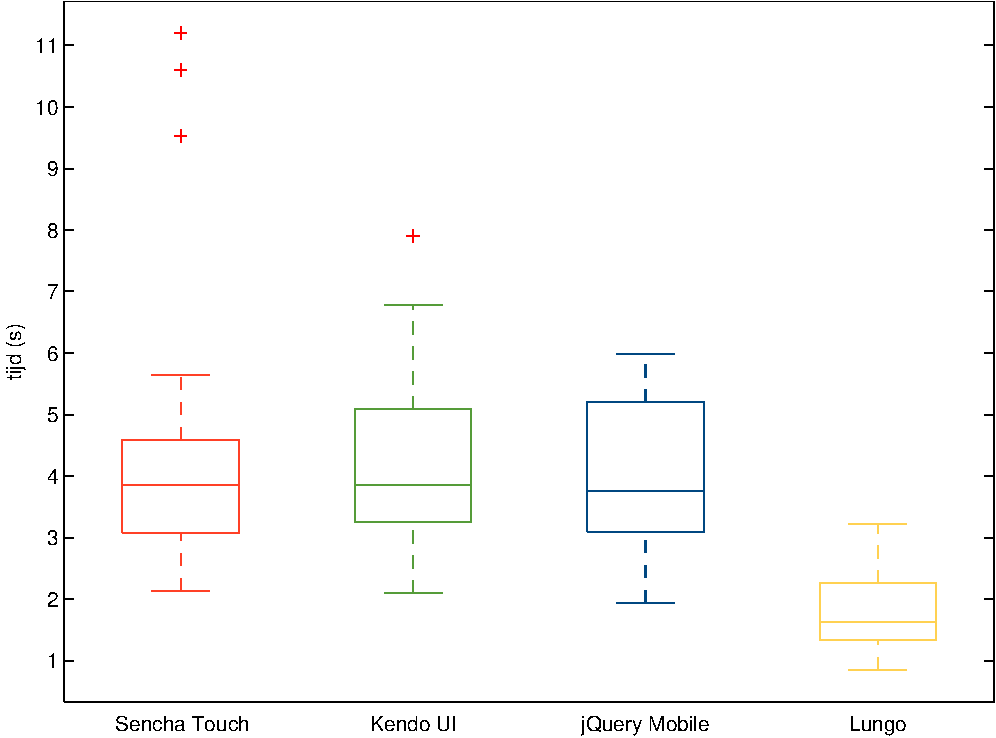
\includegraphics[width=0.85\textwidth]{figuren/performantie-login.pdf}
    \label{fig:performantie-login}
  }
  \quad
  \subfloat[Loginapplicatie uit cache]{
    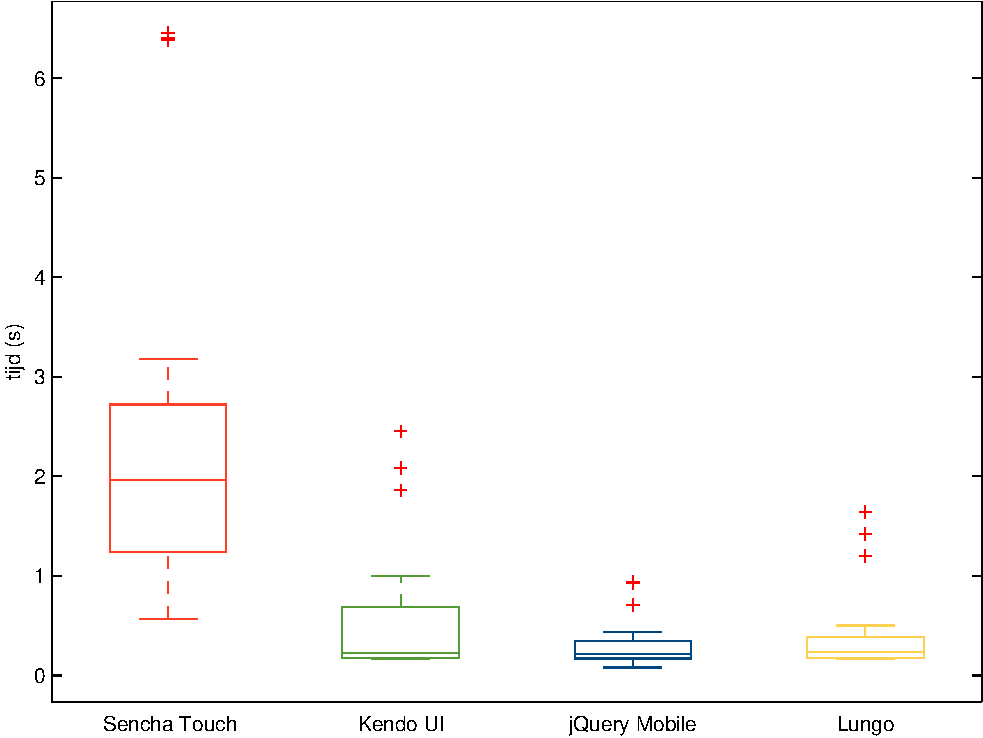
\includegraphics[width=0.85\textwidth]{figuren/performantie-login-cache.pdf}
    \label{fig:performantie-login-cache}
  }
  \caption{Downloadtijden van de loginapplicatie.}
  \label{fig:performantie-login-boxplot}
\end{figure}

\paragraph{Loginapplicatie}
\lungo{} behaalt de snelste downloadtijd (zie figuur \ref{fig:performantie-login}).
\jqm{} en \kendo{} behalen respectievelijk een tweede en derde snelste downloadtijd.
\lungo{} is meer dan de helft sneller dan \jqm{}, \kendo{} of \st{}.
Deze drie raamwerken behalen quasi dezelfde downloadtijd.
\st{} is het traagst.
De grootte van de bibliotheek domineert de werkelijk geschreven code van de loginapplicatie.
Hierdoor bepaalt de grootte van de bibliotheek van het raamwerk (zie tabel~\ref{tabel:raamwerken-tabel}) het merendeel van de totale downloadgrootte.
Raamwerken met een ontwerppatroon hebben een grotere \js{}-bestand.
Pure \js{}-gedreven raamwerken moeten alle HTML-code ter plaatse genereren, hierdoor is hun bibliotheek ook groter dan andere raamwerken.
De verwachting is dat downloadgrootte evenredig is met de downloadtijd.

%TODO tabel updaten + besluit herbekijken
\begin{table}
\centering
\pgfplotstabletypeset[
  begin table=\begin{tabular}{p{8cm} p{0.8cm} p{0.8cm} p{0.8cm} p{0.8cm} p{0.3cm}},
  end table=\end{tabular},
  skip coltypes=true,
  col sep=comma,
  string type,
  header=true,
  columns={Bibliotheek,ST,Kendo,jQM,Lungo},
  columns/Bibliotheek/.style={column name=\textbf{Bibliotheek}, column type={l}},
  columns/ST/.style={column name=\textbf{\sta}, column type={l}},  
  columns/jQM/.style={column name=\textbf{\jqma}, column type={l}},    
  columns/Kendo/.style={column name=\textbf{\kendoa}, column type={l}},   
  columns/Lungo/.style={column name=\textbf{\lungoa}, column type={l}}, 
  every head row/.style={
    before row=\toprule,
    after row=\midrule},
  every last row/.style={
  	before row=\midrule,
    after row=\bottomrule}
]{tabellen/bibliotheken.csv}
\caption{Groottes.}
\label{tabel:evaluatie-performantie-groottes}
\end{table}


\paragraph{Loginapplicatie uit cache}
Als naar de versie uit cache wordt gekeken, scoren \kendo{}, \jqm{} en \lungo{} hetzelfde (zie figuur \ref{fig:performantie-login-cache}).
Daarentegen behaalt \st{} telkens een veel tragere tijd.
Enerzijds komt dit doordat de drie eerstgenoemde raamwerken enkel gebruik maken van HTML5 Application Cache.
\st{} voegt het Delta Update mechanisme toe aan HTML5 Application Cache.
Dit mechanisme wil voorkomen dat bij een kleine aanpassing in de code,  alle bestanden opnieuw moeten worden opgehaald die in het \term{manifest} bestand staan opgelijst.
De \term{Micro-loader} is verantwoordelijk voor het asynchroon ophalen van alle benodigde \js{}- en CSS-bestanden.
Na het bouwen van een applicatie met Sencha Cmd,  zullen de gewijzigde bestanden gearchiveerd worden en worden de veranderingen tussen elke versie opgeslagen.
Na het laden van de applicatie, zal de \code{Micro-loader} met een GET-verzoek controleren op wijzigingen.
Dit GET-verzoek zal de grootste tijd voor zijn rekening nemen bij de downloadtijden bij applicaties uit de cache.
\st{} heeft er dus voor gekozen om aan performantie in te boeten ten voordele van het update mechanisme~\cite{Nguyen2012}.

\kendo{}, \jqm{} en \lungo{} gebruiken Yeoman om de applicatie te bouwen.
De webapplicaties gemaakt in \st{} gebruiken daarentegen Sencha Cmd.

%%%%%%%%%%%%%%%%%%

\subsection{Gebruikerservaring}
\label{sec:evaluatie-gebruikerservaring}

\begin{table}
\centering
\pgfplotstabletypeset[
  begin table=\begin{tabular}{p{8cm} p{0.8cm} p{0.8cm} p{0.8cm} p{0.8cm} p{0.3cm}},
  end table=\end{tabular},
  skip coltypes=true,
  col sep=comma,
  string type,
  header=true,
  columns={Apparaat,ST,Kendo,jQM,Lungo},
  columns/Apparaat/.style={column name=\textbf{Apparaat}, column type={l}},
  columns/ST/.style={column name=\textbf{\sta}, column type={l}},  
  columns/jQM/.style={column name=\textbf{\jqma}, column type={l}},    
  columns/Kendo/.style={column name=\textbf{\kendoa}, column type={l}},   
  columns/Lungo/.style={column name=\textbf{\lungoa}, column type={l}},   
  every head row/.style={
    before row=\toprule,
    after row=\midrule},
  every last row/.style={
  	before row=\midrule,
    after row=\bottomrule}
]{tabellen/performantie-gebruikerservaring.csv}
\caption{Gebruikerservaring van het scrollen door een lange lijst.}
\label{tabel:evaluatie-performantie-gebruikerservaring}
\end{table}

In tabel \ref{tabel:evaluatie-performantie-gebruikerservaring} wordt de totaalscore voor de gebruikerservaring getoond.
\st{} behaalt de maximale score.
Dit wil zeggen dat op alle toestellen het scrollen door de lijst van \st{} het vlotst werd ervaren.
\jqm{} werd zes keer als tweede beste beoordeeld. 
Op de \htc{} liep \kendo{} vlotter,  op de \ipadi{} was \lungo{} nummer twee.
De lijst genereren met \kendo{} op iOS-toestellen was onmogelijk omdat de applicatie de browser liet crashen.
De reden waarom alsook de grens van het aantal lijstelementen wanneer \kendo{} crasht op iOS-toestellen werd door tijdsbudget niet gecontroleerd.
Een mogelijke denkpiste is dat \kendo{} een overhead genereerd die het maximale toegelaten geheugen voor het iOS-besturingssysteem overschrijdt.
Op Android toestellen kon de \kendo{} lijst echter wel worden getoond.
De score van \kendo{} is dus slechts voor vier apparaten.

%%%%%%%%%%%%%%%%%%

\subsection{Duiding}
\label{sec:evaluatie-performantie-duiding}

In wat volgt zullen metrieken worden besproken die de score van de performantie zullen duiden.
De data van de metrieken is enerzijds weergegeven in tabel~\ref{tabel:performantie-verklaring} die de score met Google PageSpeed en grootte toont.
Anderzijds wordt op figuur~\ref{fig:performantie} de gemiddelde downloadtijd getoond voor zowel de POC als loginapplicatie.

\begin{table}
\centering
\pgfplotstabletypeset[
  begin table=\begin{tabular}{p{8cm} p{1cm} p{1cm} p{1cm} p{1cm}},
  end table=\end{tabular},
  skip coltypes=true,
  col sep=comma,
  string type,
  header=true,
  columns={Performantiemetrieken,jQM,ST,Kendo,Lungo},
  columns/Performantiemetrieken/.style={column name=\textbf{Performantie}, column type={l}},  
  columns/ST/.style={column name=\textbf{\sta}, column type={c}},
  columns/jQM/.style={column name=\textbf{\jqma}, column type={c}},
  columns/Kendo/.style={column name=\textbf{\kendoa}, column type={c}},
  columns/Lungo/.style={column name=\textbf{\lungoa}, column type={c}},
  every head row/.style={
    before row=\toprule,
    after row=\midrule},
  every last row/.style={
    after row=\bottomrule}
]{tabellen/performantie/performantie-verklaring.csv}
\caption{Duiding bij performantie van de loginapplicatie.}
\label{tabel:performantie-verklaring}
\end{table}


\begin{figure}
 \centering
 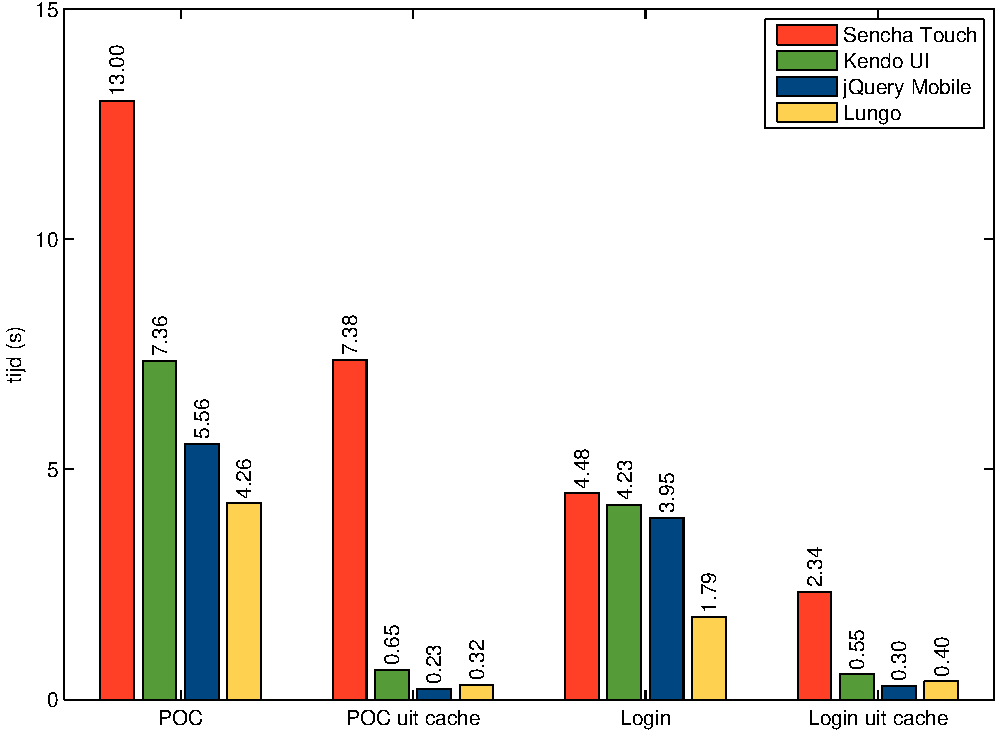
\includegraphics[width=\textwidth]{figuren/performance-nl.pdf}
 \caption{Gemiddelde downloadtijd van POC,  POC uit cache,  login en login uit cache voor elk raamwerk.}
 \label{fig:performantie}
\end{figure}

\paragraph{Downloadtijd POC versus loginapplicatie}
Op figuur \ref{fig:performantie} wordt de gemiddelde downloadtijd van de POC en login, zowel gewoon als uit cache, voor de vier raamwerken getoond.
Voor de gemiddelde downloadtijd per apparaat en per raamwerk wordt verwezen naar appendix \ref{app:performantie}.

%%% De cache factor van ST is constant (gemiddeld 1,8)
%%% De andere raamwerken hebben een beduidend grotere cache factor 

De tragere downloadtijd van \st{},  zoals geconcludeerd door de downloadtijd van de login applicatie, wordt bevestigd.
Het verschil van downloadtijden voor de POC wordt nog uitvergroot.
Het mechanisme voor het updaten van de cache zal \st{} nog meer vertragen bij de POC.

Indien \st{} buiten beschouwing wordt gelaten, duurt de eerste keer laden van de POC gemiddeld $5,73\unit{s}$. 
Het laden van de versie uit cache duurt slechts gemiddeld $400\unit{ms}$.
De eerste keer laden van de loginapplicatie duurt gemiddeld $3,32\unit{s}$.
Indien deze uit cache komt, duurt dit gemiddeld nog slechts gemiddeld $420\unit{ms}$.

Indien enkel de downloadtijd in rekening wordt gebracht en \st{} buiten beschouwing wordt gelaten, kan er gezien worden dat de downloadtijden $< 10\unit{s}$,  dit zijn aanvaardbare tijden in domein van gebruiksvriendelijkheid~\cite{Nielsen1993}.
De gebruiker zal de vertraging waarnemen maar de aandacht niet verliezen.
Het initieel laden van de POC implementatie met \st{} moet van een laadscherm worden voorzien omdat de downloadtijd $> 10\unit{s}$.


\paragraph{Google Page Speed}
De score op 100 die Google Page Speed~\cite{Morgan2011} aan de applicatie toekent kan in tabel~\ref{tabel:performantie-verklaring} worden teruggevonden.
\st{} scoort het best ($96$),  gevolgd door \lungo{} ($82$),  \kendo{}($73$) en \jqm{}($71$).

Er kan geconcludeerd worden dat Sencha Cmd de applicatie optimaal weet te bouwen,  er is het minst plaats voor verbetering.
Hoewel \st{} de meeste tijd vraagt om te laden, zal het hierna sneller werken.
Dit wordt bevestigd in de voorbije testen.

Alle implementaties worden door Google Page Speed aangeraden een tekenset te specificeren en gebruik te maken van het cachegeheugen van de browser.
Dit laatste is een suggestie om de maximale duur van documenten in de cache een week in de toekomst te zetten.
De huidige implementaties hebben een vervaldatum van slechts tien minuten.
Beide werkpunten hebben volgens Google Page Speed een lage prioriteit.
Alle raamwerken buiten \st{} worden aangeraden om de \js-code uitgesteld te parsen.
Bij \kendo{} en \jqm{} heeft dit werkpunt een hogere prioriteit in tegenstelling tot \lungo{}.
Dit komt omdat \lungo{} maar een kleiner aantal bytes moet verwerken.
De implementatie van \st{} wordt ook aangeraden om vraagtekens uit URLs te verwijderen.
Dit zou de oorzaak kunnen zijn voor het niet-cachen van bestanden.

\paragraph{Downloadgrootte}
De PCAP-bestanden die werden gebruikt om de downloadtijd op te meten, bevatten ook de grootte van de pakketten die moeten worden opgehaald.
Omdat pakketten verloren gaan, zullen ontvangen bestanden incompleet zijn en moeten ze worden herverzonden.
Hierdoor zal het aantal ontvangen bytes variëren van meting tot meting.
De performantietesten werden op acht toestellen uitgevoerd en elke test werd drie keer uitgevoerd.
Het gemiddelde van alle downloadgroottes bepaalt de grootte zoals deze kan worden teruggevonden in tabel~\ref{tabel:performantie-verklaring}.
\kendo{} moest de meeste data ophalen ($296.50$~kB),  gevolgd door \st{} ($247.59$~kB), \jqm{} ($185.43$~kB) en \lungo{} ($59.75$~kB).
\section{Vergelijkingsoverzicht}
\label{sec:evaluatie-spinnenweb}

Figuur \ref{fig:spinnenweb-final} toont een overzicht van de scores van de vier raamwerken op de vijf criteria in de vorm van een spinnenweb.
De formules van de vergelijkingscriteria voor het plotten van het spinnenweb kunnen teruggevonden worden in sectie \ref{sec:vergelijking-spinnenweb}.
Daar werden de gerelativeerde formules voorgesteld om een score tussen $0$ en $1$ te bekomen.
Ook werden de formules voor productiviteit en performantie geïnverteerd omdat voor deze criteria geldt:  hoe lager de score, hoe beter het raamwerk.

\begin{figure}
  \centering
  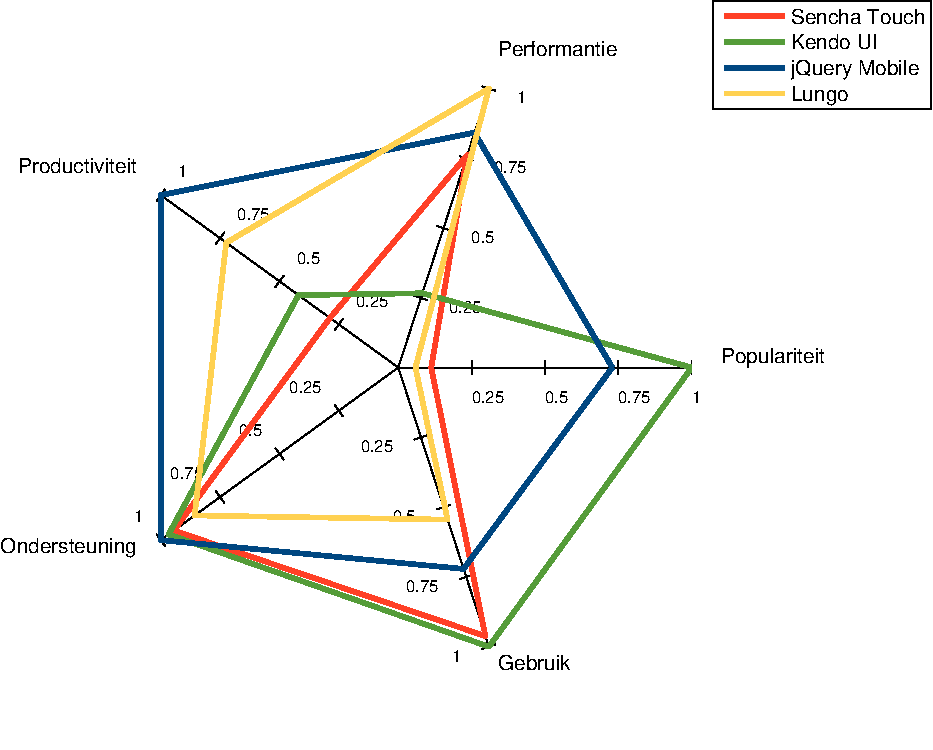
\includegraphics[width=\textwidth]{figuren/spidergraph-final-nl.pdf}
  \caption{Overzicht met de vijf vergelijkingscriteria.}
  \label{fig:spinnenweb-final}
\end{figure}



% De oppervlakten van de vier vijfhoeken is de volgende:
% \begin{description}
% %nieuwste data
%  \item [\jqm{}] $1.76$  0.858697389122251
%  \item [\kendo{}] $1.31$ 0.730739926739927
%  \item [\lungo{}] $0.90$ 0.636930206334082
%  \item [\st{}] $0.76$  0.613893381347723
% \end{description}
     
              

In wat volgt zullen de raamwerken besproken worden volgens de total score voor alle criteria.
Hiervoor werd formule \ref{eq:rel-totaal} gebruikt waar de scores van de criteria worden opgeteld.


\jqm{} heeft de beste score ($86\%$) en is de winnaar.
Een van de belangrijkste factoren die \jqm{} tot winnaar maakt is het feit dat er geen ontwerppatroon wordt afgedwongen.
Dit maakt dat de leercurve veel lager ligt ten voordele van de productiviteit.
Ook een betere documentatie en omkadering maakt \jqm{} productiever.
De grotere populariteit in vergelijking met \lungo{} maakt \jqm{} aantrekkelijker als er geen ontwerppatroon noodzakelijk is.
De afwezigheid van een ontwerppatroon brengt echter twee nadelen met zich mee.
Ten eerst zal het raamwerk minder functionaliteit kunnen aanbieden.
Door plug-ins en HTML5-kenmerken zal dit gebrek aan functionaliteit toch beperkt blijven.
Een tweede nadeel is de code die moet geschreven worden bij gebruik van het \jqm{} raamwerk.
\jqm{} is opmaakgedreven waarbij veel HTML-code moet worden geschreven met grote verbositeit.
Dit maakt het linken van HTML- met \js{}-code moeilijker.

% jQM volgt % Waarom kiezen voor jqm:
% +/- geen architectuur (
    % minder gebruik
    % lagere leercurve (veel HTML, link met js is het lastigst)
    % meer code schrijven (error prone)
% + zeer populair (jQuery core) zie stackoverlow => vragen worden door een hele community opgelost (geen payed support)
% als een easy (geen architectuur) raamwerk + populair (belangrijke klanten,  gekend op social media)

\kendo{} bekleedt de tweede plaats met een score van $73\%$.
In tegenstelling tot \jqm{} heeft het wel een ontwerppatroon en is het dus meer bruikbaar.
De score van de productiviteit bevindt zich onder de helft maar in vergelijking met \st{} scoort het beter.
Het grote nadeel van \kendo{},  wat niet in het spinnenweb kan worden gezien,  is de hoge kost voor een licentie.
Het feit dat \kendo{} niet \term{open-source} is, reflecteert zich echter niet in de populariteit.
Van alle vier raamwerken is \kendo{} het minst performant.
De downloadtijden waren lager in vergelijking met \st{} maar de crashes op iOS-toestellen zorgden voor een lage gebruikservaring.
Het feit dat \kendo{} een \term{native look-and-feel} aanbiedt is een belangrijk kenmerk maar dit kan ook niet op het spinnenweb worden teruggevonden.
De iOS-lay-out is sterk gelijkend op de echte iOS-lay-out.
Dit was bij Android minder geslaagd.

% kendo is winnaar (uitstekend op pop, gebruik en ondersteuning % Waarom kiezen voor kendo:
% - architectuur => minder productief maar meer bruikbaar
% - hoge licentiekost => professionele support. Ondanks niet open source toch populiar (meest populair)
% + native look-and-feel => downloadtijden stijgen?  meer op native applicatie (positieve impact niet geevalueerd) (iOS lay-out sterk gelijkend op
%echte iOS,  Android minder gelijkend, Blackberry en windows niet bekeken)

\lungo{} heeft de derde score ($64\%$).
Op drie van de vijf criteria scoort \lungo{} het slechtst.
Er is geen ontwerppatroon opgelegd en weer kan dit voor- en nadeel zowel in productiviteit en gebruik opgemerkt worden.
De voordelen bij productiviteit zijn echter minder dan bij \jqm{} omdat de ondersteuning en documentatie minimaal is.
De nadelen bij gebruik zijn dan weer uitvergroot omdat er niet zoveel functionaliteit en plug-ins als bij \jqm{} konden worden teruggevonden.
Positief is dan weer dat \lungo{} de beste downloadtijden behaalde omdat \quo{}, de \js{}-bibliotheek van \lungo{},  geoptimaliseerd is voor mobiele apparaten.
De testen op gebruikservaring zwakte de performantie van \lungo{} af.
\lungo{} is veruit het minst populair.
Dit kan zowel met de literatuur als met sociale netwerken bevestigd worden.

% tweede is lungo % Waarom kiezen voor lungo:
% - productiviteit => verkeerde indruk (zonder voorkennis / sumire documentatie maakt het moeilijk)
% - support => niet bij oudere android OS (2.3) X)(marktwaarde android 2.3 tov alle devices)X% van de devices vallen dan uit de boot
% + performatie zeer positief => quo js geoptimaliseerd (bedrijf gespecialiseerd in mobile user experience)! (weinig support help hier ook)
% nauwelijks bekend (literatuur, social networks (zie populariteit), ...)

\st{} is volgens de gekozen criteria het slechtste raamwerk ($61\%$).
De combinatie van het MVC-ontwerppatroon en \js-gedreven opmaak maken \st{} zowel het minst productief als minst performant in vergelijking met de andere raamwerken.
Alle HTML-code wordt door het raamwerk zelf aangemaakt waardoor de \js-bestanden zeer groot zijn.
De downloadtijden waren dan ook opmerkelijk langer door het Delta Update mechanisme.
De gebruikservaring gaf echter het tegenovergestelde resultaat want na de lange downloadtijd reageerde \st{} het beste.
De tools die Sencha aanbiedt om ontwikkelaars te helpen (Sencha Architect en Sencha Cmd) blijken niet voldoende om het verschil met andere raamwerken te verkleinen.
Met de tools leren werken, is een leerproces op zich.
Hoewel de ondersteuning van \st{} hoog is, moet er opgemerkt worden dat het afhankelijk is van de WebKit \term{engine}.
Toestellen met een standaard browser die deze \term{engine} niet bevatten, zoals Windows Phone,  kunnen \st{} niet gebruiken.

% Sencha (nergens numero uno) % Waar niet kiezen voor st:
% + / - Tools voorhanden (Sencha Cmd / Architect ) om programmeren makkelijker te maken maar tools niet even handig (of betalend)
% - Javascript driven maakt het lastig (alle simple HTML moet in js worden geschreven): meeste lijnen JS + grote bibliotheek => minder performant
% - gebaseerd op webkit => geteste toestellen hadden dit wel (windows phone geen webkit)


%%%%%%%%%%%%%%%%% NIET BESPROKEN

% besluiten  (de getallen zijn geen procenten)
% 1) Kendo: 1,51 
% 2) Lungo: 1,14
% 3) jQM: 1,03
% 4) ST: 0,62

%%%%%%%%%%%%%%%%%%%%%%%%%%


% daarna de bindparagraaf door onze 2 improvents (productiviteit en performantie)
% referen naar de nieuwe formules in de respectievelijke secties
% nieuwe formules voor het bereken van het relatieve waarden voor de respectievelijke formules
% tonen van de finale grafiek


%nieuwe zaken finaal versus initieel:
%Productiviteit
  % jqm naar eerste plaats,  andere boeten in (raamwerk met architectuur komen achteraan,  stemt overeen met verwachtingen)
%Performantie:
  %Kendo: iOS crash van lange lijst: performantie daalt van 40% naar 25%
  %Sencha : Performantie verhoogt want gebruikservaring maximaal

%jQM naar eerst plaats, rest schuift een plaats door (buiten st)
% snelle ontwikkeling die performant is en overal ondersteund wordt geen payed support nodig hebt en geen geavanceerde features wil implementeren





\chapter{Besluit}
\label{chap:besluit}

\section{Conclusie} % 1 pagina % Sander
% - wat we gedaan hebben, onze doelen, hebben we de beste gevonden?
% - we hebben dat gevonden, ….

Deze thesistekst bestaat uit twee doelstellingen.
Een eerste doel is het definiëren van een methodologie om HTML5-raamwerken met elkaar te vergelijken.
Het tweede doel omvat de effectieve vergelijking van de raamwerken zelf.

De uitgelichte raamwerken zijn \st{}, \kendo{},  \jqm{} en \lungo{}.
\st{} bouwt op het MVC-ontwerppatroon en is \js-gedreven.
Het raamwerk is gratis en heeft zowel een commerciële als \term{open-source} licentie.
\kendo{} dwingt het MVVM-ontwerppatroon af en is zowel \js- als opmaakgedreven.
Een licentie voor het gebruik van \kendo{} kost $\$699$.
\jqm{} en \lungo{} hebben geen ontwerppatroon en zijn beide opmaakgedreven.
Beide raamwerken zijn \term{open-source}.

Vijf criteria werden gekozen om de vergelijkende studie uit te voeren:  populariteit,  productiviteit,  gebruik,  ondersteuning en performantie.
Elk criterium werd voorzien van een formule om een score te berekenen voor het criterium.
In samenspraak met Capgemini werd een POC opgesteld die werknemers toelaat onkosten toe te voegen.
Deze werd gebruikt om het gebruik en de ondersteuning te drijven.  
Om populariteit te meten werd naar de activiteit van de raamwerken op sociale netwerken gekeken.
De tijd om een loginapplicatie te ontwikkelen, bepaalde de productiviteit.
De POC werd onderverdeeld in $13$ uitdagingen en $38$ deeluitdagingen om de functionaliteit van het raamwerk te testen en het gebruik te quoteren.
Vervolgens werd een subset van de uitdagingen getest op acht verschillende mobiele toestellen om de ondersteuning te controleren.
Ten slotte bepaalden de downloadtijd en de gebruikerservaring van de loginapplicatie de performantie.
De gebruikerservaring bepaalt hoe vlot het gaat om door een lange lijst te scrollen.
De scores van de vijf criteria voor de vier raamwerken werden in één spinnenweb ondergebracht.

Na evaluatie is \jqm{} het beste raamwerk op basis van de gekozen criteria, gevolgd door \kendo{}, \lungo{} en \st{}.
Deze volgorde werd bepaald door de scores van alle criteria op te tellen.
\jqm{} heeft als belangrijkste troeven de hoge productiviteit en performantie doordat het enerzijds zeer goed gedocumenteerd is en anderzijds geen ontwerppatroon afdwingt.
Dit laatste is echter een nadeel waardoor het minder scoort op gebruik.
\kendo{} heeft als belangrijkste troef het gebruik doordat het een ontwerppatroon afdwingt.
Het scoort echter ondermaats op performantie door het crashen van lange lijsten op iOS.
\lungo{} behaalt op geen enkel criterium de maximumscore.
Het behaalde echter wel de beste downloadtijd bij performantie doordat het raamwerk is geoptimaliseerd voor mobiel gebruik.
\st{} is het minst productief en minst performant in vergelijking met de andere raamwerken.
Daarentegen scoort \st{} het best op het vlak van gebruikerservaring.
Door het afdwingen van een ontwerppatroon scoort het quasi evengoed als \kendo{} op vlak van gebruik.
Alle onderzochte raamwerken scoren zeer goed op ondersteuning.


\section{Geleerde lessen} % 1 pagina 
Bij het uitvoeren van een vergelijkende studie is de keuze van de vergelijkingscriteria bepalend voor het resultaat van het onderzoek.
Daarbij is het belangrijk om reeds bestaande literatuur grondig te controleren.
Zo werd er in het begin te specifiek naar papers gezocht omtrent het vergelijken van HTML5-raamwerken.
Meer algemene methodologieën om software te vergelijken moesten worden gezocht waaruit criteria konden worden hergebruikt.

Bij het opzetten van criteria is het van groot belang dat de manier waarop deze criteria zullen worden getoetst, zeer gedetailleerd worden neergeschreven.
De exacte formules van de criteria werden pas tijdens de evaluatie vastgelegd.
Pas dan werd de nood van een formele notatie duidelijk.
Ook is het belangrijk om op voorhand de elementen van een vergelijkende studie uit te testen alvorens de vergelijkingscriteria vast te leggen.
Hierdoor kunnen iteraties over de criteria vermeden worden als blijkt dat ze niet toepasbaar zijn.
Een initiële vertrouwdheid met de raamwerken had er ook voor gezorgd dat de criteria meer kenmerken van de raamwerken zouden bevatten.
De raamwerken die steunen op een ontwerppatroon konden op die manier meer bevoordeeld worden door bijvoorbeeld uitbreidbaarheid te introduceren, zoals dat ook in de ISO-25010 wordt gebruikt.

Een andere geleerde les is dat er in het uitvoeren van de evaluatie veel werk kruipt.
Echter, het interpreteren en begrijpen van de resultaten duurde zowaar nog langer.
Ook het opsporen en verbeteren van eigen fouten is zeer tijdsrovend.
Door op een consistente en gestructureerde methode de evaluatie te voltooien, moet het aantal fouten tot een minimum worden beperkt.

Er werden tot slot nog twee praktische zaken geleerd.
Het opmeten van tijd en het gebruik van logboeken vereist een zekere vorm van discipline.
Het eerste was noodzakelijk om de productiviteit van het raamwerk te toetsen.
De tijdbudgetten die nodig waren moesten gemakkelijk kunnen worden gereconstrueerd.
De logboeken werden gebruikt bij de implementatie van de POC en moesten bij de evaluatie het gebruikscriterium drijven.
Een tweede praktisch punt gaat over de samenwerking tussen beide auteurs.
Het is geen gemakkelijke opgave om als twee individuen continu op gelijke hoogte te zitten.
Dit vraagt enorm veel onderlinge gesprekken met duidelijke communicatie.
Discipline, sociale netwerken en andere technologieën zoals Google Drive en \gh{} hielpen de communicatie te verbeteren.

\section{Verder onderzoek} % 1 pagina % Tim
Er kan verder gezocht worden naar de oorzaak waarom bepaalde zaken zeer opmerkelijk waren of waarom ze niet lukten tijdens de vergelijking.
Zo was er enerzijds de crash van de 850 lijstitems van \kendo{} op iOS.
Hier kan gezocht worden naar de oorzaak van de crash, maar tevens kan ook gezocht worden naar de grens van het aantal lijstitems waarbij dat het wel lukt.
Anderzijds was er een opmerkelijke waarneming bij de performantie van de applicaties uit cache. 
Zo ligt bijvoorbeeld de gemiddelde downloadtijd van de login uit cache hoger dan deze van de POC voor \jqm{} en \lungo{}. 

Ook kunnen nieuwe raamwerken worden toegevoegd aan de vergelijking.
Hierdoor vergroot ten eerste de grootte van de vergelijking, maar kan ten tweede ook de methode telkens opnieuw worden getoetst met deze nieuwe raamwerken.
Daarnaast komen van de reeds vergeleken raamwerken geregeld nieuwe versies uit.
Zo is het ook mogelijk om de evolutie in de rangschikking van de vier vergeleken raamwerken over de tijd te bekijken.
Mogelijk kan de rangschikking veranderen bij het uitbrengen van nieuwe versies of plug-ins.

De huidige methode omvat vijf vergelijkingscriteria die worden gedreven door de POC.
Verder onderzoek kan deze POC uitbreiden met extra kenmerken zoals Pull\&Refresh.
Dit loopt in de lijn om ook andere gebeurtenissen te gebruiken dan alleen maar de \term{tap} gebeurtenis.
Andere gebeurtenissen zijn bijvoorbeeld \term{double tap}, \term{swipe}, \term{hold}, maar ook gebeurtenissen waar meerdere vingers voor nodig zijn zoals \term{rotate}.
Daarnaast is ook de integratie van HTML5-kenmerken zoals GPS, \term{push events}, \term{drag and drop}, video en audio in de raamwerken zeker het onderzoeken waard.

Naast het toevoegen van extra kenmerken aan de POC, kunnen criteria ook op andere manieren gecontroleerd worden.
Nu worden bij ondersteuning enkel apparaten met een Android- of iOS-besturingssysteem gebruikt.
Dit kan worden vervangen of uitgebreid naar andere besturingssystemen zoals Windows Phone en BlackBerry~OS.
Een andere voorbeeld is dat voor de downloadtijd bij performantie Wifi werd gebruikt voor de verbinding.
Andere verbindingsmogelijkheden zoals 3G kunnen worden gebruikt en hierdoor kunnen andere resultaten bekomen worden.
Een derde voorbeeld is de rendertijden die worden gebruikt bij performantie.
Deze konden niet worden opgemeten bij \st{} en \lungo{}.
Aanpassingen aan de broncode zouden het opmeten van rendertijden wel kunnen toelaten.
Daarnaast kan het gebruikte alternatief dat bepaalt hoe vlot het gaat om door een lange lijst te scrollen, ook verbeterd worden.
Als laatste kunnen ook de lijnen effectief geschreven code worden gebruikt bij productiviteit. 

Een andere onderzoekspiste is om nieuwe criteria toe te voegen.
Zo kan bijvoorbeeld het criterium uitbreidbaarheid worden onderzocht.
Dit criterium omvat hoe gemakkelijk het gaat om de bestaande applicatie geïmplementeerd in een bepaald raamwerk uit te breiden.
Een te onderzoeken hypothese hierbij is dat raamwerken die een ontwerppatroon afdwingen beter zullen scoren dan raamwerken zonder ontwerppatroon.
Een bijkomende hypothese is dat de totale score van raamwerken die een ontwerppatroon afdwingen zal stijgen en deze van raamwerken zonder ontwerppatroon zal dalen.
Dit komt doordat de ene worden afgestraft op productiviteit en de andere op uitbreidbaarheid.
Mogelijk kan de rangschikking van de vier onderzochte raamwerken veranderen.
Anderzijds kan ook een criterium worden toegevoegd die kijkt naar het finale resultaat van het raamwerk.
Zo kunnen bepaalde raamwerken de \term{native look-and-feel} van mobiele besturingssystemen  nabootsen, andere raamwerken bieden dan weer standaard een frisse hedendaagse lay-out.

Andere onderzoeksvragen kunnen een stap terugnemen door bijvoorbeeld af te vragen of het baterijverbruik door webapplicaties een probleem vormt.
De bekomen data kan worden vergeleken met \term{native} en hybride applicaties.
Deze laatste vergelijking kan zelfs veralgemeend worden waardoor een vergelijking tussen web-, \term{native} en hybride applicaties zich opdringt. 


%%% Local Variables: 
%%% mode: latex
%%% TeX-master: "masterproef"
%%% End: 


%% Bijlagen
\appendixpage*          
\appendix
\chapter{Poster}
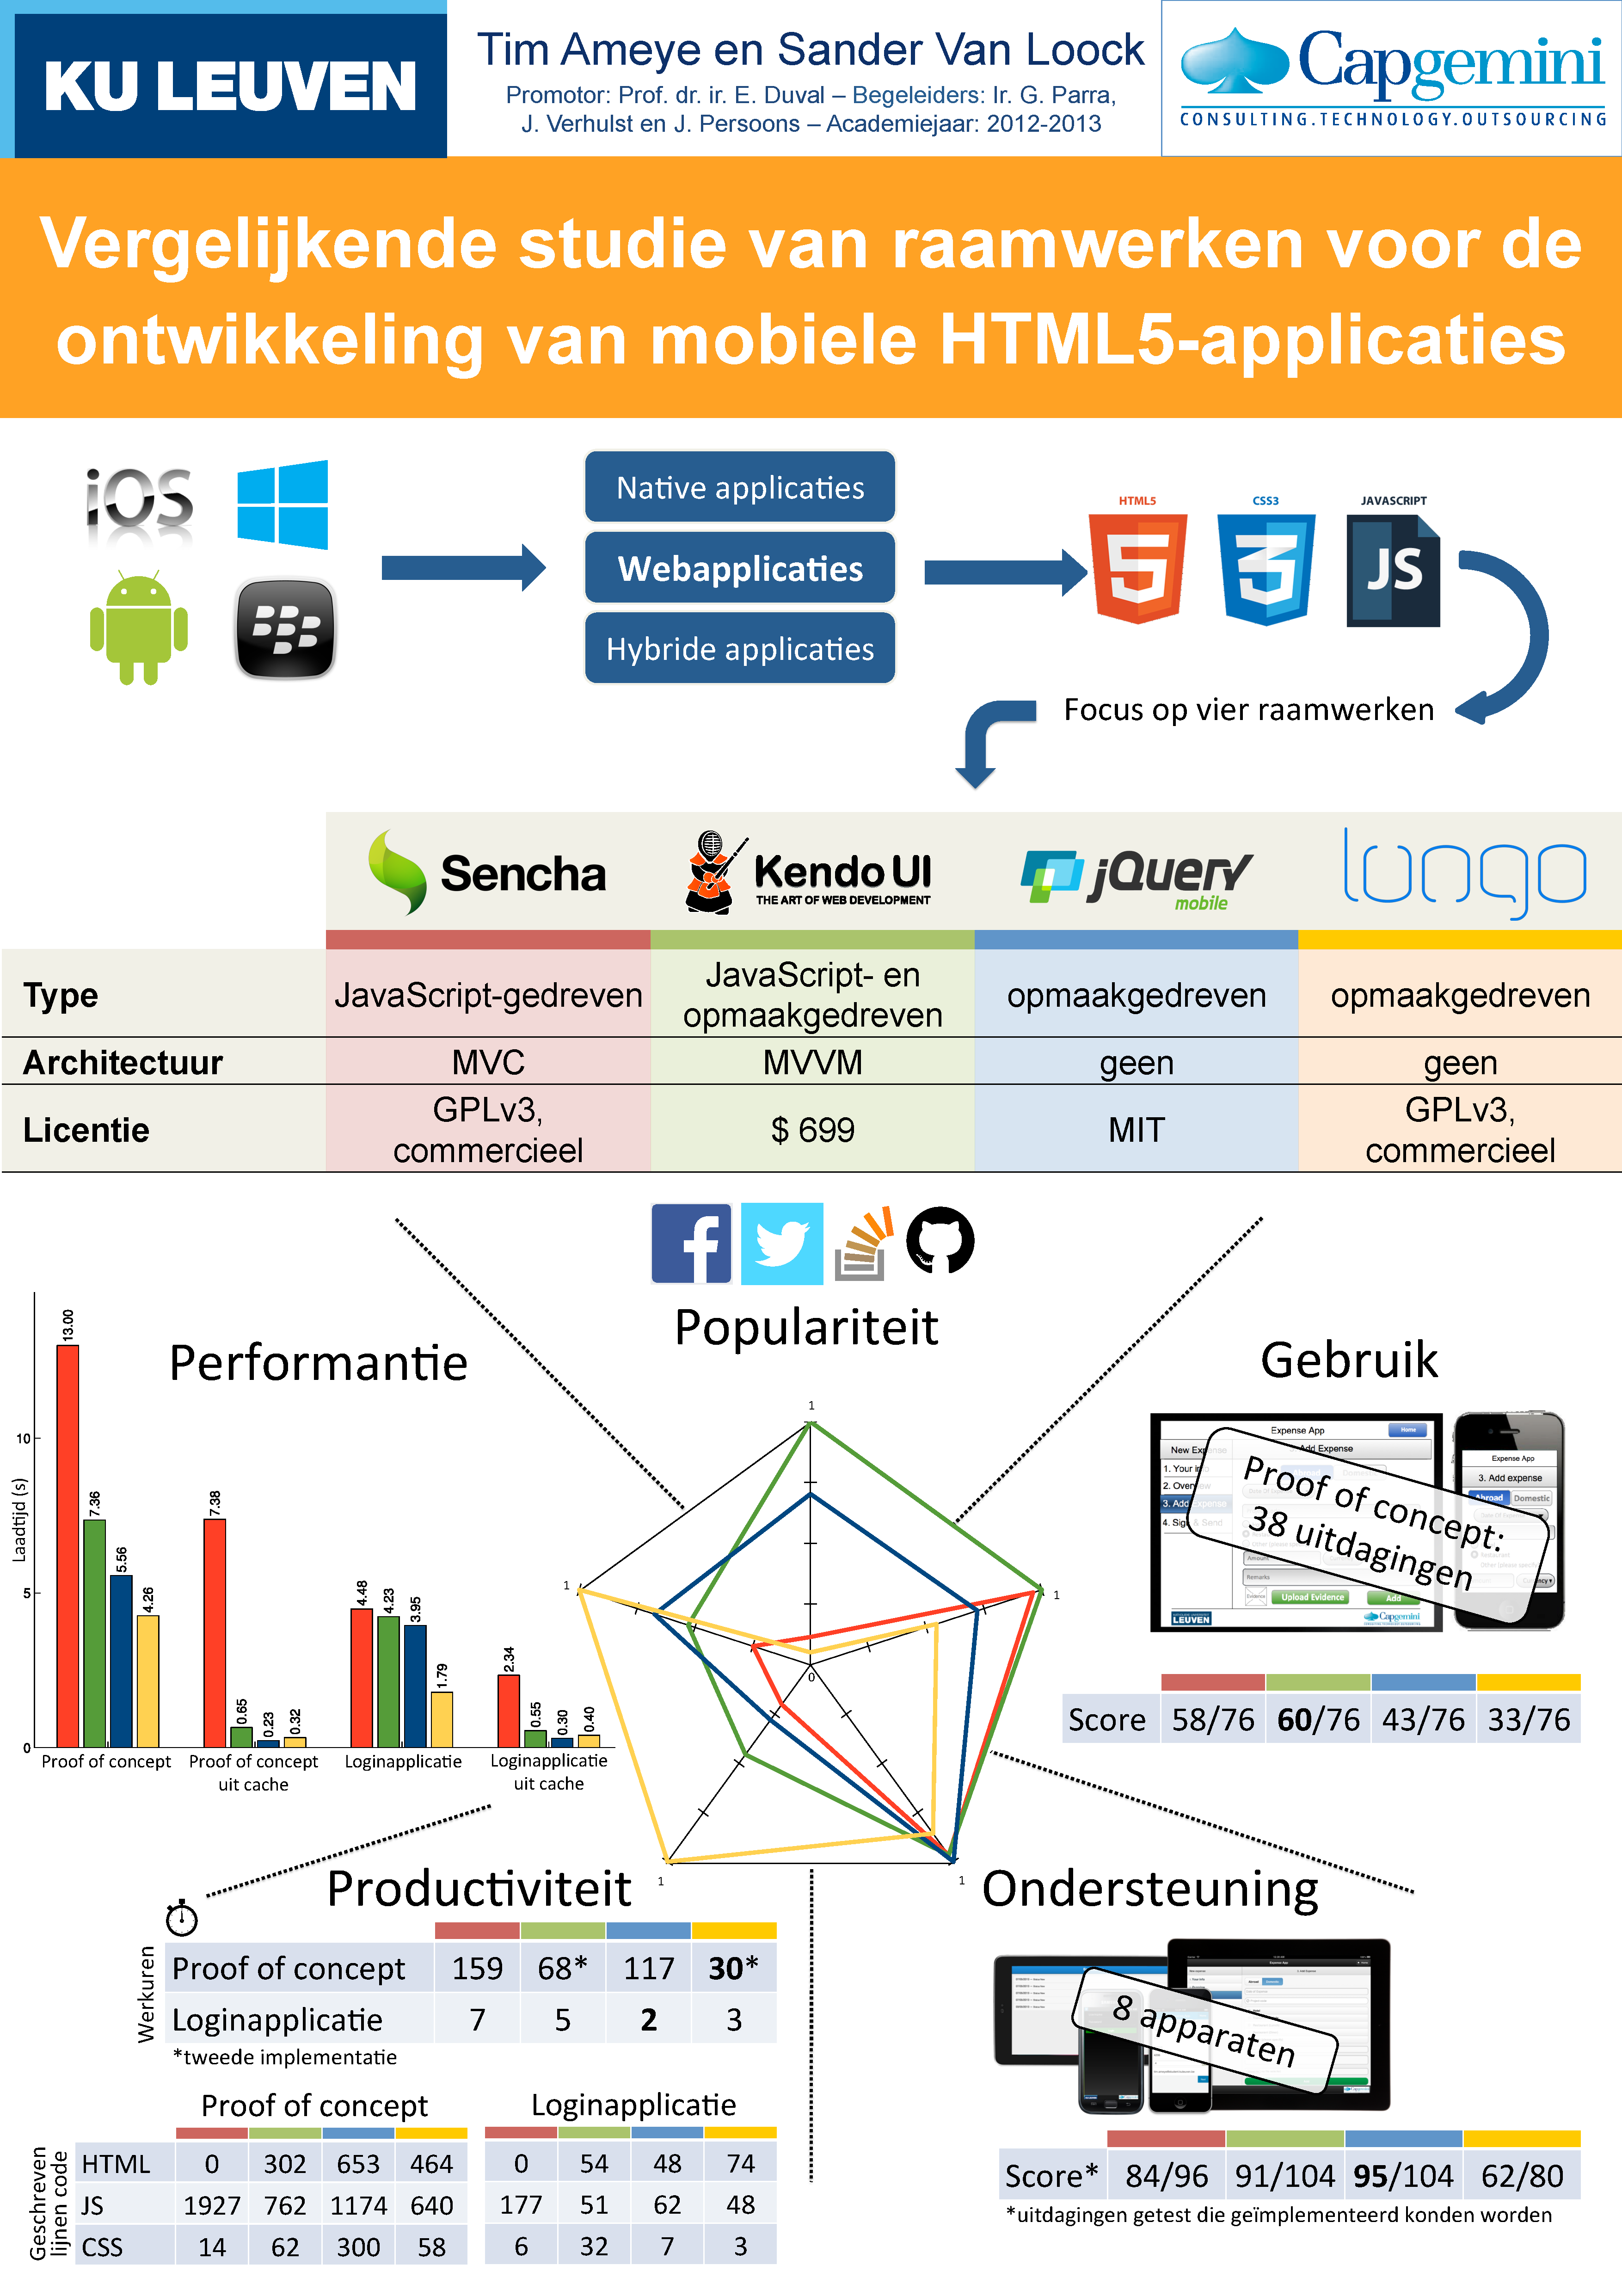
\includepdf[pages={1}]{../Poster/htmobiel.pdf}
\chapter{Wetenschappelijk artikel}
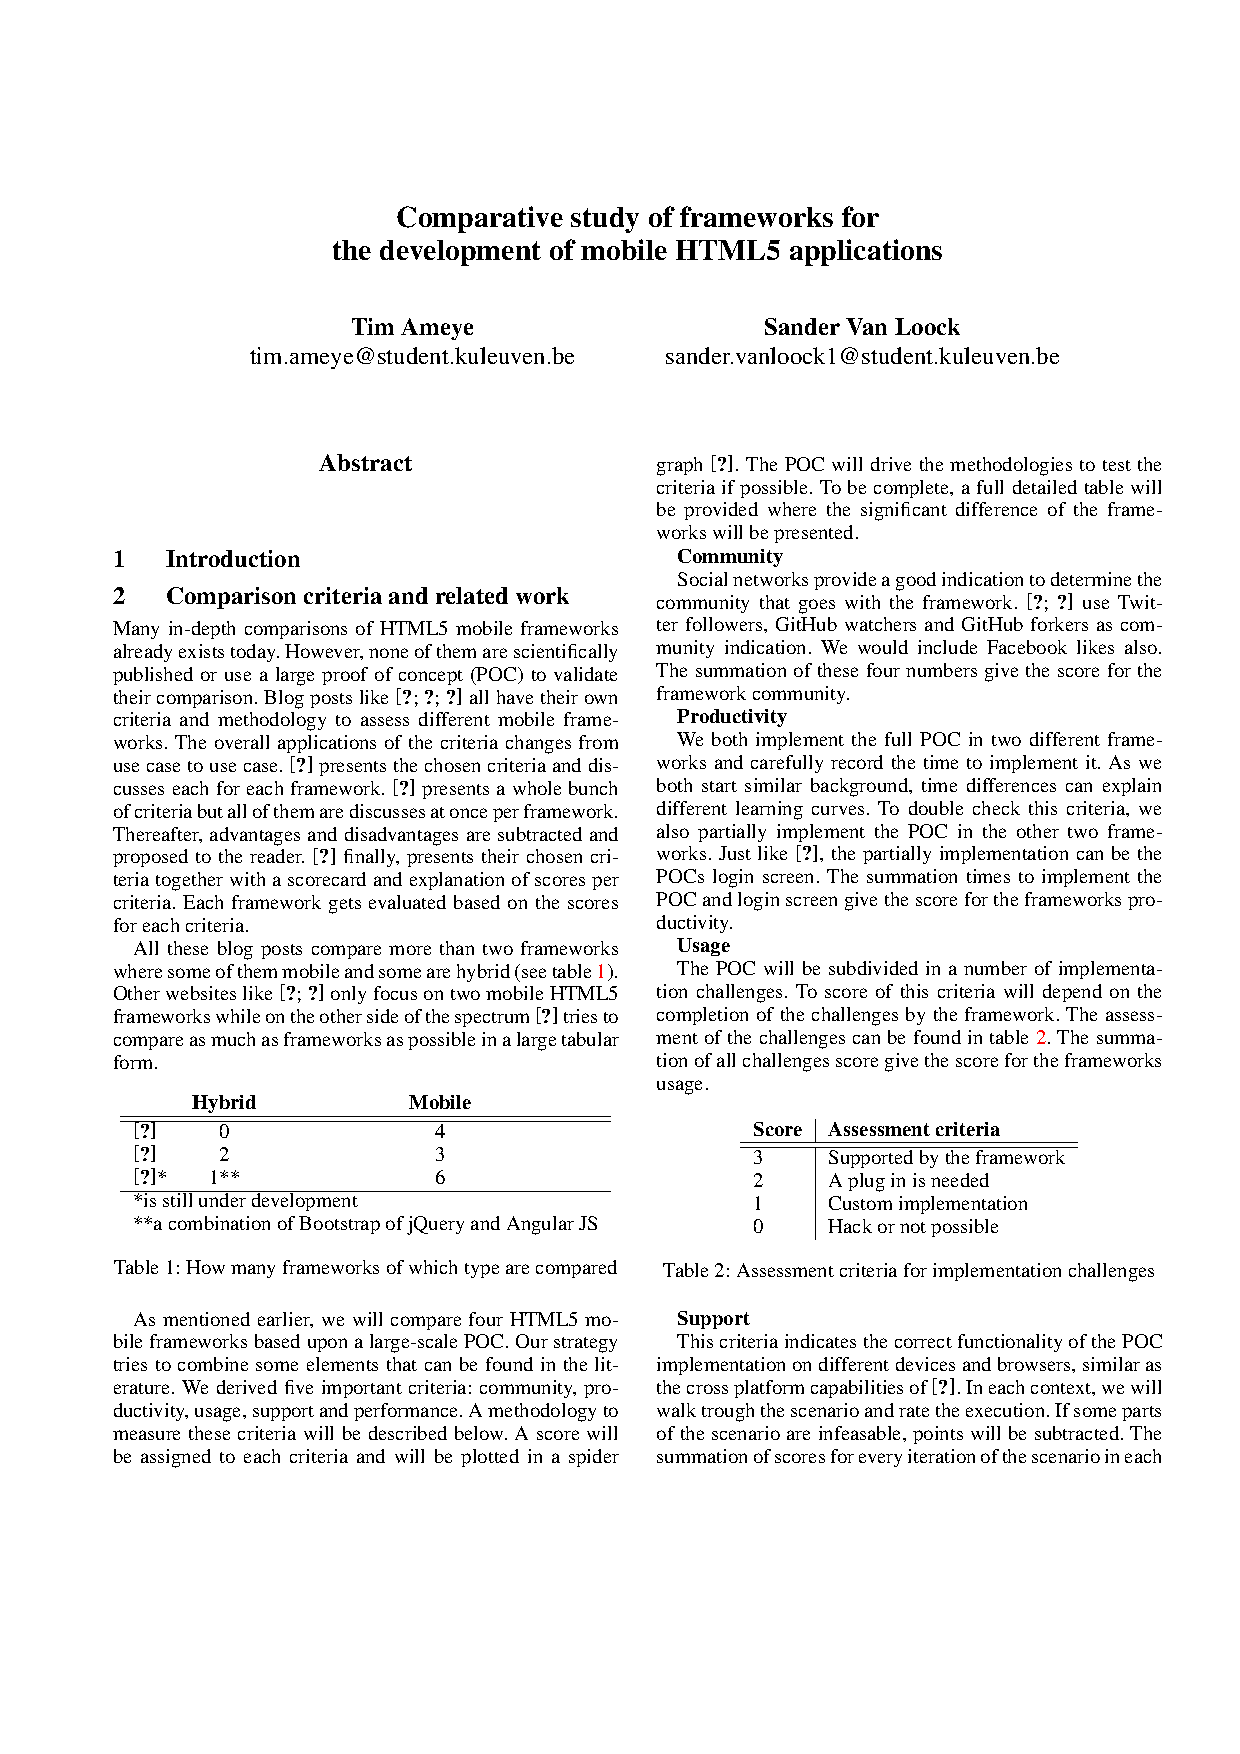
\includepdf[pages={1-11}]{../Artikel/artikel.pdf}
\chapter{Ondersteuning}
\label{app:ondersteuning}

In deze appendix wordt een gedetailleerd overzicht gegeven van de ondersteuning van de uitdagingen op de acht apparaten: 
\htc{} (zie tabel~\ref{tabel:evaluatie-ondersteuning-htc}),
\gtab{} (zie tabel~\ref{tabel:evaluatie-ondersteuning-galaxytab}),
\gs{} (zie tabel~\ref{tabel:evaluatie-ondersteuning-galaxys}),
\nexus{} (zie tabel~\ref{tabel:evaluatie-ondersteuning-nexus}),
\ipadi{} (zie tabel~\ref{tabel:evaluatie-ondersteuning-ipad1}),
\ipadiii{} (zie tabel~\ref{tabel:evaluatie-ondersteuning-ipad3}),
\iphoneiii{} (zie tabel~\ref{tabel:evaluatie-ondersteuning-iphone3}),
\iphoneiv{} (zie tabel~\ref{tabel:evaluatie-ondersteuning-iphone4}).

\begin{table}[H]
\centering
\resizebox{13.5cm}{!} {
\pgfplotstabletypeset[
  begin table=\begin{tabular}{p{8cm} p{1cm} p{1cm} p{1cm} p{1cm}},
  end table=\end{tabular},
  skip coltypes=true,
  col sep=comma,
  string type,
  header=true,
  columns={Uitdaging,jQM,ST,Kendo,Lungo},
  columns/Uitdaging/.style={column name=\textbf{Uitdaging}, column type={l}},  
  columns/jQM/.style={column name=\textbf{\jqma}, column type={c}},
  columns/ST/.style={column name=\textbf{\sta}, column type={c}},
  columns/Kendo/.style={column name=\textbf{\kendoa}, column type={c}},
  columns/Lungo/.style={column name=\textbf{\lungoa}, column type={c}},
  every head row/.style={
    before row=\toprule,
    after row=\midrule},
  every last row/.style={
  	before row=\toprule,
 	after row=\bottomrule}
]{tabellen/ondersteuning/htc.csv}
}
\caption{Ondersteuning op \htc.}
\label{tabel:evaluatie-ondersteuning-htc}
\end{table}

\begin{table}[H]
\centering
\resizebox{13.5cm}{!} {
\pgfplotstabletypeset[
  begin table=\begin{tabular}{p{8cm} p{1cm} p{1cm} p{1cm} p{1cm}},
  end table=\end{tabular},
  skip coltypes=true,
  col sep=comma,
  string type,
  header=true,
  columns={Uitdaging,jQM,ST,Kendo,Lungo},
  columns/Uitdaging/.style={column name=\textbf{Uitdaging}, column type={l}},  
  columns/jQM/.style={column name=\textbf{\jqma}, column type={c}},
  columns/ST/.style={column name=\textbf{\sta}, column type={c}},
  columns/Kendo/.style={column name=\textbf{\kendoa}, column type={c}},
  columns/Lungo/.style={column name=\textbf{\lungoa}, column type={c}},
  every head row/.style={
    before row=\toprule,
    after row=\midrule},
  every last row/.style={
  	before row=\toprule,
 	after row=\bottomrule}
]{tabellen/ondersteuning/galaxytab.csv}
}
\caption{Ondersteuning op \gtab.}
\label{tabel:evaluatie-ondersteuning-galaxytab}
\end{table}

\begin{table}[H]
\centering
\resizebox{13.5cm}{!} {
\pgfplotstabletypeset[
  begin table=\begin{tabular}{p{8cm} p{1cm} p{1cm} p{1cm} p{1cm}},
  end table=\end{tabular},
  skip coltypes=true,
  col sep=comma,
  string type,
  header=true,
  columns={Uitdaging,jQM,ST,Kendo,Lungo},
  columns/Uitdaging/.style={column name=\textbf{Uitdaging}, column type={l}},  
  columns/jQM/.style={column name=\textbf{\jqma}, column type={c}},
  columns/ST/.style={column name=\textbf{\sta}, column type={c}},
  columns/Kendo/.style={column name=\textbf{\kendoa}, column type={c}},
  columns/Lungo/.style={column name=\textbf{\lungoa}, column type={c}},
  every head row/.style={
    before row=\toprule,
    after row=\midrule},
  every last row/.style={
  	before row=\toprule,
 	after row=\bottomrule}
]{tabellen/ondersteuning/galaxys.csv}
}
\caption{Ondersteuning op \gs.}
\label{tabel:evaluatie-ondersteuning-galaxys}
\end{table}

\begin{table}[H]
\centering
\resizebox{13.5cm}{!} {
\pgfplotstabletypeset[
  begin table=\begin{tabular}{p{8cm} p{1cm} p{1cm} p{1cm} p{1cm}},
  end table=\end{tabular},
  skip coltypes=true,
  col sep=comma,
  string type,
  header=true,
  columns={Uitdaging,jQM,ST,Kendo,Lungo},
  columns/Uitdaging/.style={column name=\textbf{Uitdaging}, column type={l}},  
  columns/jQM/.style={column name=\textbf{\jqma}, column type={c}},
  columns/ST/.style={column name=\textbf{\sta}, column type={c}},
  columns/Kendo/.style={column name=\textbf{\kendoa}, column type={c}},
  columns/Lungo/.style={column name=\textbf{\lungoa}, column type={c}},
  every head row/.style={
    before row=\toprule,
    after row=\midrule},
  every last row/.style={
  	before row=\toprule,
 	after row=\bottomrule}
]{tabellen/ondersteuning/nexus.csv}
}
\caption{Ondersteuning op \nexus.}
\label{tabel:evaluatie-ondersteuning-nexus}
\end{table}

\begin{table}[H]
\centering
\resizebox{13.5cm}{!} {
\pgfplotstabletypeset[
  begin table=\begin{tabular}{p{8cm} p{1cm} p{1cm} p{1cm} p{1cm}},
  end table=\end{tabular},
  skip coltypes=true,
  col sep=comma,
  string type,
  header=true,
  columns={Uitdaging,jQM,ST,Kendo,Lungo},
  columns/Uitdaging/.style={column name=\textbf{Uitdaging}, column type={l}},  
  columns/jQM/.style={column name=\textbf{\jqma}, column type={c}},
  columns/ST/.style={column name=\textbf{\sta}, column type={c}},
  columns/Kendo/.style={column name=\textbf{\kendoa}, column type={c}},
  columns/Lungo/.style={column name=\textbf{\lungoa}, column type={c}},
  every head row/.style={
    before row=\toprule,
    after row=\midrule},
  every last row/.style={
  	before row=\toprule,
 	after row=\bottomrule}
]{tabellen/ondersteuning/ipad1.csv}
}
\caption{Ondersteuning op \ipadi.}
\label{tabel:evaluatie-ondersteuning-ipad1}
\end{table}

\begin{table}[H]
\centering
\resizebox{13.5cm}{!} {
\pgfplotstabletypeset[
  begin table=\begin{tabular}{p{8cm} p{1cm} p{1cm} p{1cm} p{1cm}},
  end table=\end{tabular},
  skip coltypes=true,
  col sep=comma,
  string type,
  header=true,
  columns={Uitdaging,jQM,ST,Kendo,Lungo},
  columns/Uitdaging/.style={column name=\textbf{Uitdaging}, column type={l}},  
  columns/jQM/.style={column name=\textbf{\jqma}, column type={c}},
  columns/ST/.style={column name=\textbf{\sta}, column type={c}},
  columns/Kendo/.style={column name=\textbf{\kendoa}, column type={c}},
  columns/Lungo/.style={column name=\textbf{\lungoa}, column type={c}},
  every head row/.style={
    before row=\toprule,
    after row=\midrule},
  every last row/.style={
  	before row=\toprule,
 	after row=\bottomrule}
]{tabellen/ondersteuning/ipad3.csv}
}
\caption{Ondersteuning op \ipadiii.}
\label{tabel:evaluatie-ondersteuning-ipad3}
\end{table}

\begin{table}[H]
\centering
\resizebox{13.5cm}{!} {
\pgfplotstabletypeset[
  begin table=\begin{tabular}{p{8cm} p{1cm} p{1cm} p{1cm} p{1cm}},
  end table=\end{tabular},
  skip coltypes=true,
  col sep=comma,
  string type,
  header=true,
  columns={Uitdaging,jQM,ST,Kendo,Lungo},
  columns/Uitdaging/.style={column name=\textbf{Uitdaging}, column type={l}},  
  columns/jQM/.style={column name=\textbf{\jqma}, column type={c}},
  columns/ST/.style={column name=\textbf{\sta}, column type={c}},
  columns/Kendo/.style={column name=\textbf{\kendoa}, column type={c}},
  columns/Lungo/.style={column name=\textbf{\lungoa}, column type={c}},
  every head row/.style={
    before row=\toprule,
    after row=\midrule},
  every last row/.style={
  	before row=\toprule,
 	after row=\bottomrule}
]{tabellen/ondersteuning/iphone3.csv}
}
\caption{Ondersteuning op \iphoneiii.}
\label{tabel:evaluatie-ondersteuning-iphone3}
\end{table}

\begin{table}[H]
\centering
\resizebox{13.5cm}{!} {
\pgfplotstabletypeset[
  begin table=\begin{tabular}{p{8cm} p{1cm} p{1cm} p{1cm} p{1cm}},
  end table=\end{tabular},
  skip coltypes=true,
  col sep=comma,
  string type,
  header=true,
  columns={Uitdaging,jQM,ST,Kendo,Lungo},
  columns/Uitdaging/.style={column name=\textbf{Uitdaging}, column type={l}},  
  columns/jQM/.style={column name=\textbf{\jqma}, column type={c}},
  columns/ST/.style={column name=\textbf{\sta}, column type={c}},
  columns/Kendo/.style={column name=\textbf{\kendoa}, column type={c}},
  columns/Lungo/.style={column name=\textbf{\lungoa}, column type={c}},
  every head row/.style={
    before row=\toprule,
    after row=\midrule},
  every last row/.style={
  	before row=\toprule,
 	after row=\bottomrule}
]{tabellen/ondersteuning/iphone4.csv}
}
\caption{Ondersteuning op \iphoneiv.}
\label{tabel:evaluatie-ondersteuning-iphone4}
\end{table}

%%% Local Variables: 
%%% mode: latex
%%% TeX-master: "masterproef"
%%% End: 

\chapter{Performantie}
\label{app:performantie}

In deze appendix wordt een gedetailleerd overzicht gegeven van de performantie voor de vier raamwerken op de acht apparaten: 
\st{} (zie \ref{app:performantie-st}),
\kendo{} (zie \ref{app:performantie-kendo}),
\jqm{} (zie \ref{app:performantie-jqm}),
\lungo{} (zie \ref{app:performantie-lungo}).

%%%%%%%%

\section{\st}
\label{app:performantie-st}
\begin{figure}
  \centering
  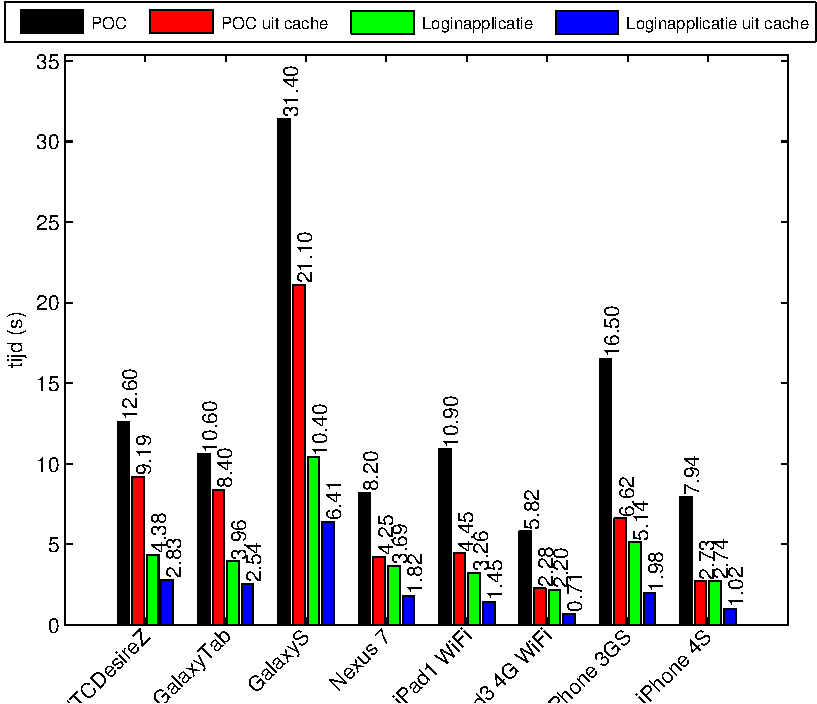
\includegraphics[width=0.75\textwidth]{figuren/performance-st.pdf}
  \caption{Gemiddelde downloadtijden van \st{} voor POC,  POC uit cache,  loginapplicatie en loginapplicatie uit cache voor elk apparaat.}
  \label{fig:performantie-st}
\end{figure}

Op figuur~\ref{fig:performantie-st} wordt de gemiddelde downloadtijd van \st{} getoond op elk apparaat.
Voor de POC is een dalende downloadtijd waarneembaar wanneer het Android-apparaat recenter wordt.
De downloadtijd van de POC op de \gs{} duurde gemiddeld $31.43$s.
Gemiddeld moeten Android toestellen $5$ seconden langer laden in vergelijking met iOS toestellen.
Dit gemiddelde wordt sterk beïnvloed door de trage downloadtijd van de \gs{}.

Een opmerking die bij \st{} moet worden gemaakt, is dat AJAX-verzoeken van een \code{proxy} naar een ander domein altijd vooraf worden gegaan met een OPTIONS-verzoek.
Dit is een verzoek om informatie over de beschikbare opties van het communicatiekanaal op te vragen.
Standaard zet \st{} de \code{X-Requested-With} op XMLHttpRequest en hierdoor zal de browser een OPTIONS-verzoek als \term{preflight} sturen.

%Setting custom headers on XHR requests triggers a preflight request. %http://remysharp.com/2011/04/21/getting-cors-working/
%http://stackoverflow.com/questions/10236056/when-loading-a-store-in-sencha-touch-2-how-can-i-stop-the-additional-options-ht
% POST /resources/userService/login?_dc=1368367749599 HTTP/1.1
% Host: kulcapexpenseapp.appspot.com
% Connection: keep-alive
% Content-Length: 54
% Origin: http://sandervanloock.github.io
% User-Agent: Mozilla/5.0 (X11; Linux i686) AppleWebKit/537.11 (KHTML, like Gecko) Chrome/23.0.1271.64 Safari/537.11
% Content-Type: application/x-www-form-urlencoded; charset=UTF-8
% Accept: */*
% Referer: http://sandervanloock.github.io/HTMobieL/Sencha/build/ExpenseApp/production/index.html
% Accept-Encoding: gzip,deflate,sdch
% Accept-Language: nl-NL,nl;q=0.8,en-US;q=0.6,en;q=0.4
% Accept-Charset: ISO-8859-1,utf-8;q=0.7,*;q=0.3
% 
% Accept:*/*
% Accept-Charset:ISO-8859-1,utf-8;q=0.7,*;q=0.3
% Accept-Encoding:gzip,deflate,sdch
% Accept-Language:nl-NL,nl;q=0.8,en-US;q=0.6,en;q=0.4
% Connection:keep-alive
% Content-Length:23
% Content-Type:application/x-www-form-urlencoded; charset=UTF-8
% Host:kulcapexpenseapp.appspot.com
% Origin:http://sandervanloock.github.io
% Referer:http://sandervanloock.github.io/HTMobieL/Sencha/build/ExpenseApp/production/index.html
% User-Agent:Mozilla/5.0 (X11; Linux i686) AppleWebKit/537.11 (KHTML, like Gecko) Chrome/23.0.1271.64 Safari/537.11
% X-Requested-With:XMLHttpRequest

%%%%%%%%

\section{\kendo}
\label{app:performantie-kendo}

\begin{figure}
  \centering
  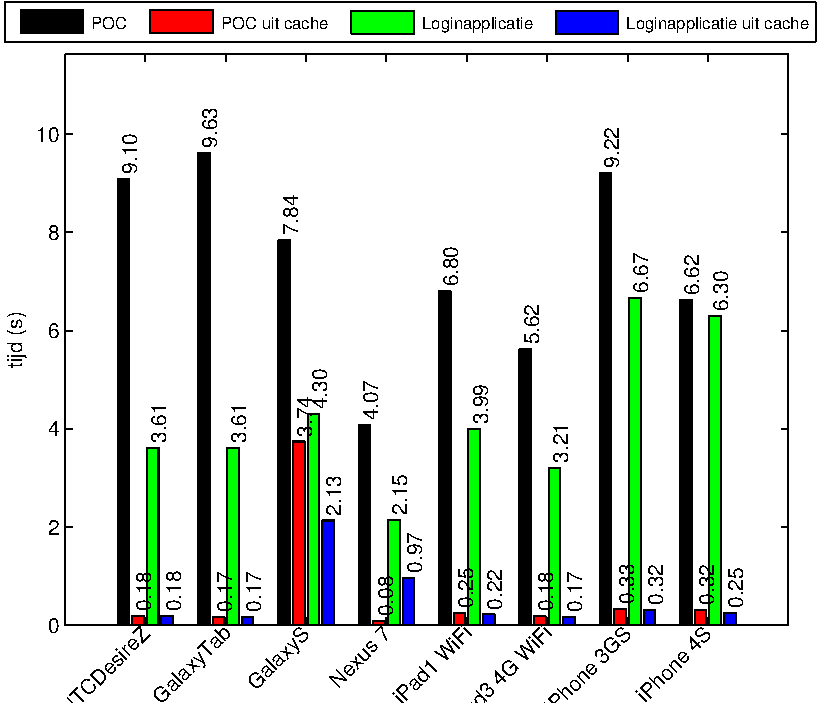
\includegraphics[width=0.75\textwidth]{figuren/performance-kendo.pdf}
  \caption{Gemiddelde downloadtijden van \kendo{} voor POC,  POC uit cache,  loginapplicatie en loginapplicatie uit cache voor elk apparaat.}
  \label{fig:performantie-kendo}
\end{figure}

Op figuur~\ref{fig:performantie-kendo} worden de gemiddelde downloadtijd van \kendo{} getoond op elk apparaat.
De \gtab{} vertoont de hoogste downloadtijd,  gevolgd door de \iphoneiii{} en \htc.
Opmerkelijk is dat de gecachete versie van de loginapplicatie op de \nexus{} $10$ keer trager laadt dan de gecachete versie van de POC.
Het ophalen van een gecachete applicatie werkt bij de \gs{} het traagst.
Bij \kendo{} is er geen opmerkelijk verschil waarneembaar tussen Android en iOS toestellen (Android gemiddeld slechts $60$ms trager).

%%%%%%%%

\section{\jqm}
\label{app:performantie-jqm}

\begin{figure}
  \centering
  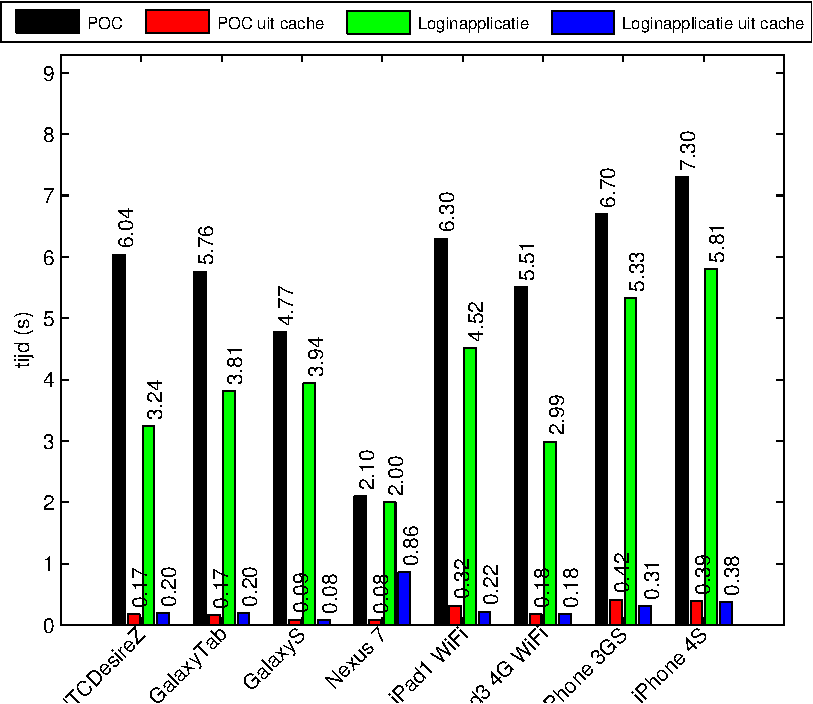
\includegraphics[width=0.75\textwidth]{figuren/performance-jquery.pdf}
  \caption{Gemiddelde downloadtijd van \jqm{} voor POC,  POC uit cache, loginapplicatie en loginapplicatie uit cache voor elk apparaat.}
  \label{fig:performantie-jqm}
\end{figure}

Op figuur~\ref{fig:performantie-jqm} wordt de gemiddelde downloadtijd van \jqm{} getoond op elk apparaat.
Voor de POC is een dalende downloadtijd waarneembaar wanneer de Android-versies op het apparaat recenter worden.
iPads dalen in de downloadtijd als het apparaat recenter wordt, daarentegen stijgt de downloadtijd bij iPhones.
Er zijn minimale verschillen bij de POC uit cache, waarbij het het langste duurt op de \iphoneiv{}.

Als de loginapplicatie wordt bekeken, wordt hetzelfde waargenomen als voor de POC.
Enkel bij de Android-apparaten wordt de downloadtijd trager, naarmate het toestel recenter wordt. 
Dit is in tegenstelling tot de POC.
Enkel de \nexus{} volgt deze trend niet.
Op de \nexus{} wordt de loginapplicatie zelfs even snel gedownload als de POC.
Een opmerkelijke waarneming is dat het op de \nexus{} langer duurt om de loginapplicatie uit cache te laden dan de volledige POC uit cache.

%%%%%%%%

\section{\lungo}
\label{app:performantie-lungo}

\begin{figure}
  \centering
  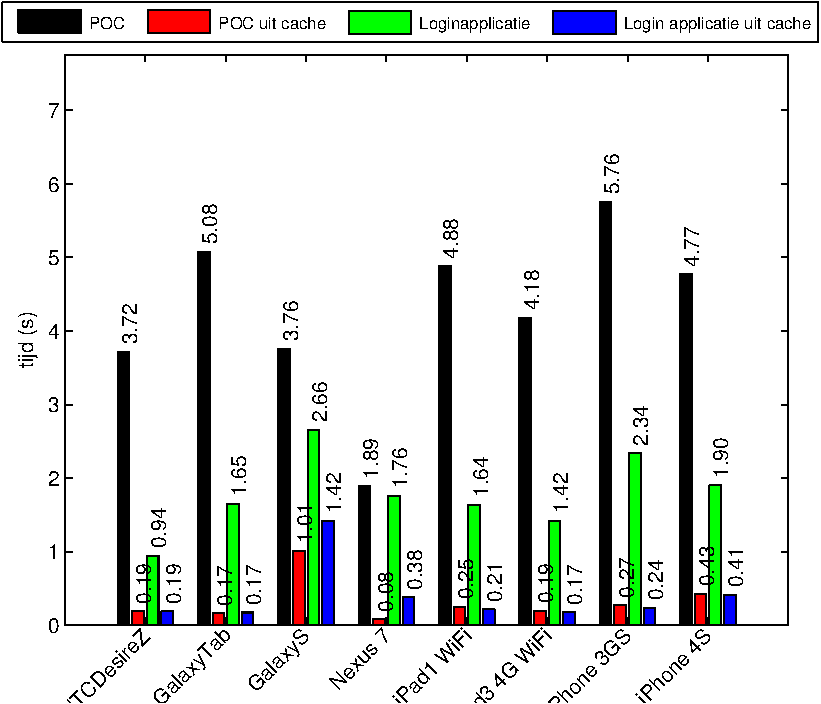
\includegraphics[width=0.75\textwidth]{figuren/performance-lungo.pdf}
  \caption{Gemiddelde downloadtijd van \lungo{} voor POC,  POC uit cache,  loginapplicatie en loginapplicatie uit cache voor elk apparaat.}
  \label{fig:performantie-lungo}
\end{figure}

Op figuur~\ref{fig:performantie-lungo} wordt de gemiddelde downloadtijd van \lungo{} getoond op elk apparaat.
Er is geen begrijpbare trend waarneembaar voor Android.
Wel is er een opmerkelijke waarneming op de \gs{}, waarbij de downloadtijden uit cache langer duren dan 1 seconde, terwijl op alle apparaten deze tijden rond de 0,25 seconden liggen.
Bij iOS daalt de downloadtijd als het toestel recenter is.
Zo is de downloadtijd op \ipadiii{} sneller dan \ipadi{}.
Het geldt ook zo dat \iphoneiv{} sneller download dan \iphoneiii{}.

%%% Local Variables: 
%%% mode: latex
%%% TeX-master: "masterproef"
%%% End: 


\backmatter
% Na de bijlagen plaatst men nog de bibliografie.
% Je kan de  standaard "abbrv" bibliografiestijl vervangen door een andere.
\makeatletter
\g@addto@macro{\UrlBreaks}{\UrlOrds}
\makeatother
\bibliographystyle{abbrv}
\bibliography{../Referenties/alles-nl}

\end{document}

%%% Local Variables: 	
%%% mode: latex
%%% TeX-master: t
%%% End: 
